
\title{Recap Database Management System (01NVVOV)}
\author{Jacopo Nasi\\
        Computer Engineer\\
        Politecnico di Torino}
\date{I Period - 2017/2018\\\bigskip\bigskip\today}

\documentclass[12pt]{article}
\usepackage[utf8]{inputenc}
\usepackage[italian]{babel}
\usepackage{geometry}
\usepackage{indentfirst} % First line indent
\usepackage{mathtools}
\usepackage{wrapfig}
\usepackage[usenames, dvipsnames]{color}
\usepackage{float}
\usepackage{amssymb}
\usepackage{ifsym}
\usepackage{listings}

\lstset{language=SQL}
% Misure Documento
\geometry{ a4paper, total={170mm,257mm},left=35mm, right=35mm, top=35mm, bottom=35mm }

\begin{document}

\begin{figure}
  \centering
  
\includegraphics[width=10cm]{images/polito.pdf}
\end{figure}

\maketitle

\newpage
\tableofcontents

\newpage
{\noindent \Large \textbf{License}\bigskip}

This work is licensed under a Creative Commons Attribution-NonCommercial-ShareAlike 3.0 Unported License.\\
You are free:
\begin{itemize}
  \item \textbf{to Share}: to copy, distribute and transmit the work
  \item \textbf{to Remix}: to adapt the work
\end{itemize}
Under the following conditions:
\begin{itemize}
  \item \textbf{Attribution}: you must attribute the work in the manner specified by the author or licensor (but not in any way that suggests that they endorse you or your use of the work)
  \item \textbf{Noncommercial}: you may not use this work for commercial purposes.
  \item \textbf{Share Alike}: if you alter, transform, or build upon this work, you may distribute the resulting work only under the same or similar license to this one.
\end{itemize}

\noindent More information on the Creative Commons website (http://creativecommons.org).

\begin{figure}[h!]
  \centering
  
\includegraphics[width=3cm]{images/license.png}
\end{figure}

{\noindent \Large \textbf{Acknowledgments}\bigskip}

Questo breve riepilogo non ha alcuno scopo se non quello di agevolare lo studio di me stesso, se vi fosse di aiuto siete liberi di usarlo.\\
Le fonti su cui mi sono basato sono quelle relative al corso offerto (\textbf{Database Management System (01NVVOV)}) dal Politecnico di Torino durante l'anno accademico 2017/2018.\\
Non mi assumo nessuna responsabilità in merito ad errori o qualsiasi altra cosa. Fatene buon uso!
\clearpage

\section{Database Management System}
\subsection{Introduction}

The DataBase Management System \textbf{DBMS} is a software package designed to store and manage databases. The architecture of the system is similar to the one in the figure \ref{fig:arch}.
\begin{figure}[h!]
  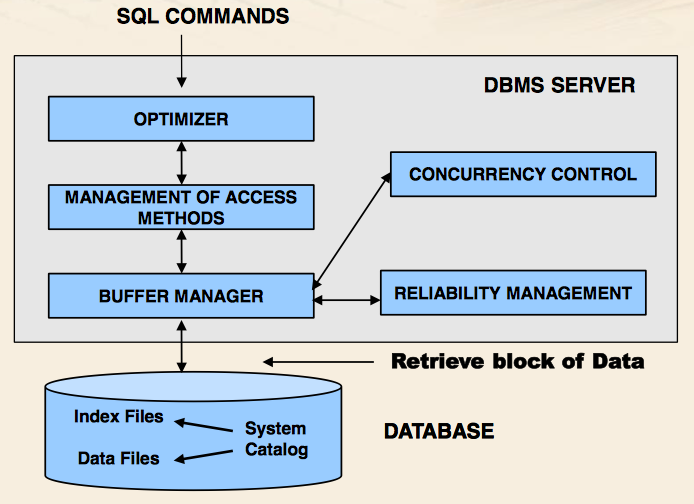
\includegraphics[width=\linewidth]{images/arch.png}
  \caption{DBMS Architecture}
  \label{fig:arch}
\end{figure}
Since the DB data part can be really big it can't fit always in the main memory (RAM) and, for this fact, is often stored in the secondary memory, like HDD. For this reason is necessary a system that define the operations to grab and manage the data from the secondary memory.\\
All the blocks has different behaviours. The \textbf{Optimizer} have multiple roles:
\begin{itemize}
  \item Define an appropriate execution strategy for accessing data to answer queries.
  \item Receives in input the SQL instructions (DML).
  \item Check the lexical, syntactical and sematical correctness (not all the errors).
  \item Translate the query in an internal algebra rappresentation.
  \item Select the "right" strategy for accesing data.
  \item Guarantees the \textbf{data independence} property in the relation model.
\end{itemize}
The \textbf{Access Method Manager} is used for physical access to data and it implements the strategy selected by the optimizer. The \textbf{Buffer Manager} instead manage the page transfert from disk to main memory and vice versa and the main memory portion that is pre-allocated to the DBMS that is shared among many applications. The \textbf{Concurrency Control} coordinate the concurrent access to data (important for write operations) to guarantess the consistency of it. The \textbf{Realiability Manager} guarantees correctness of the database content duing the system crashes, the atomic execution of a transaction and it exploits auxiliary structures (log files) the correct the database in case of failure.\\
The \textbf{transaction} is an unit of work performed by an application, it's a sequence of one or more SQL RW operation charaterized by \textit{correctness, reliability} and \textit{isolation}. The START of a transaction is typically implicit and coincides with the first SQL instruction. The END instead can be of two differents types, it can be a COMMIT that it means the correct end of a transaction, or with ROLLBACK that it means error during the execution. In this second case the DBMS needs to go back to the state at the beginning of the transaction. The rollback can be of two type suicide, when is required by the transaction, and murder when is required by the system. The transaction have four important properties:
\begin{itemize}
  \item \textbf{A}tomicity
  \item \textbf{C}onsistency
  \item \textbf{I}solation
  \item \textbf{D}urability
\end{itemize}
Atomicity means that they cannot be divided in smaller units, is not possibile to leave the system in a intermediate state of exec, guarantee by UNDO (undoes all the work perfomed, used for rollback) and REDO (redoes all work performed, used for commit the result in presence of failure). The consistency means that the transaction execution should not violate integrity constraints on a database, in case of it the system will perform solution to correct the violation. The system can be considered Isolated when the execution of a transaction is indipendent of the concurrent execution of other transaction, everything is enforced by the Concurrency Control block. The last properties means that, in presence of failures, the effect of a commited transaction IS NOT LOST, it guarantees the reliability of the DBMS and is enforced by the Reliability Manager block. % 3/9/17 @ 18:15

\subsection{Buffer Manager}
This block have a real important behaviour, it manages page transfer from disk to main memory and it's in charge of managing the DBMS buffer. The operation of the pages transfert is the bottleneck of every system and this is why this block is really important. increasing the performance of this operation could really improve the speed of the entire system.\\
The buffer is:
\begin{itemize}
  \item A large main memory block.
  \item Pre-allocated to the DBMS.
  \item Shared among executing transactions.
\end{itemize}
this part is organized in pages where the size depends on the size of the OS I/O block. There are two empirical law often used for hte management strategies:
\begin{enumerate}
  \item Data Locality: Data referenced recntly is likely to be referenced again.
  \item 20-80: The 20\% of data is RW by 80\% of transaction.
\end{enumerate}
The buffer manager keeps additional snapshot information on the current content of the buffer, it shot, for every page, the physical location of the page on the secondary memory (file identifier and block number) and two state variables, one that count of the number of trasn using the page in that time (count), and the dirty bit that is set if the page has been modified.\\ %Set No. 2 @ PAG. 8
It provides different access methods to load pages from disk and vice versa:
\paragraph{Fix Primitive} used by transactions to require access to a disk page, after the page is loaded into the buffer a pointer is returned to the requesting transaction and the Count is incremented by 1. This procedure requires an I/O operation only id the page is not already in the buffer. There are two behaviour:
\begin{itemize}
  \item Page already in buffer: Return the pointer to the data.
  \item Page not in buffer: It search a place for the page.
  \begin{enumerate}
    \item Free pages
    \item Not free pages, Count=0; if the data is dirty it performs a synchronous write on the disk.
  \end{enumerate}
\end{itemize}
\paragraph{Unfix Primitive} it tells the buffer manager that the transaction is no longer using the page and it decrease the Count.
\paragraph{Set Dirty Primitive} is tells the buffer manager that the page has been modified by the running transaction and it sets the dirty bit to 1.
\paragraph{Force Primitive} it requires a synchronous transfert of the page to the disk, when this operation is performed the transaction is suspended.
\paragraph{Flush Primitive} is an autonomous transfert of the pages on the disks, is internal to the buffer manager and is runned when the CPU is not too much loaded. It transfer the page that are not valid (count=0) or not accessed since long time.\\
The are four writing strategies:
\begin{itemize}
  \item \textbf{Steal}: The BM is allowed to select a locked page with Count=0 as victim. It writes on disk the dirty pages belonging to uncommitted trans. It can be undone.
  \item \textbf{No Steal}: The BM is not allow to steal.
  \item \textbf{Force}: All the pages are synchronous written on the disk during the commit operation.
  \item \textbf{No Force}: The pages are written asynchronously with the Flush Primitive.
\end{itemize}
The mostly used solution is \textbf{steal/no force} because of its efficency. The no force provides better I/O performance, steal may be mandatory for queries accessing a very large number of pages.

\paragraph{File System} the BM is using services provided by the file system:
\begin{itemize}
  \item Create/Delete of a file.
  \item Open/Close file.
  \item Read: It provides a direct access to a block in a file and it requires File Identifier, Block number and buffer page where to save data.
  \item Sequential Read: It provides seq. access to a fixed number of blocks in a file, it requires file identifier, strating block, number of blocks to be readed and the starting page for saving.
  \item Write and Sequential Write.
  \item Directory management.
\end{itemize} % END Block 2 - Buffer Manager

\subsection{Physical Access}
Data may be stored in different format to provide efficient query execution. The \textbf{Access Method Manager} transform the decision taken by the optimizer into sequence of physical access to data. An access method is a software module specialized for single data structure that provide primitives for read and write. The AM can select the appropriate blocks of a file to be loaded in memory and it knows the organization of data into a page.\\
There are several solution for manage the data in relational system:
\begin{itemize}
  \item Physical data storage
  \begin{itemize}
    \item Sequential Structure
    \item Hash Structure
  \end{itemize}
  \item Indexing
  \begin{itemize}
    \item Tree Structure
    \item Unclustered Hash Index
    \item Bitmap Index
  \end{itemize}
\end{itemize}

In the sequential solution the tuples are stored in a given sequential order, in the case of the heap file are sorted in the insertion order, typically append at the end of the file.
\begin{itemize}
  \item \textbf{PRO}: No wasted space, sequential read/write fast.
  \item \textbf{CONS}: Delete may cause wasted space.
\end{itemize}
this structure are frequently used jointly with unclustered indices to support search and sort operations.\\
In the ordered structures everything is sorted by the value of a given key, called sort key, it can contain one or more attributes.
\begin{itemize}
  \item \textbf{PRO}: Sort, group by, search or join operations on the sort key really fast.
  \item \textbf{CONS}: Inserting new value preserving order.
\end{itemize}
the main problem of this solution is to keep the order of the data during new data insertion. There are two main solution, the first il leaving a percentage of free space in each block during the table creation; the second one create an overflow file containing tuples which do not fit into the correct block.\\
The ordered structure are typically used with $B^{+}$-Tree clustered (primary) indices where the index key is the sort key. Are used bt the DBMS too to storing intermediate operation results. This structure provide "direct" access to data based on a key (one or more attributes). This Tree have one root node with many intermediate nodes and each node has many children. The leaf nodes provide access to data in 2 different ways:
\begin{itemize}
  \item \textbf{Clustered}: It store the data in the main memory. Used for primary key indexing. [figure \ref{fig:clu}]
  \item \textbf{Unclustered}: It store a pointer to the secondary memory of the data. Used for secondary indices. [figure \ref{fig:unclu}]
\end{itemize}
\begin{figure}[!hbpt]
  \centering
  \begin{minipage}{.45\textwidth}
    \centering
    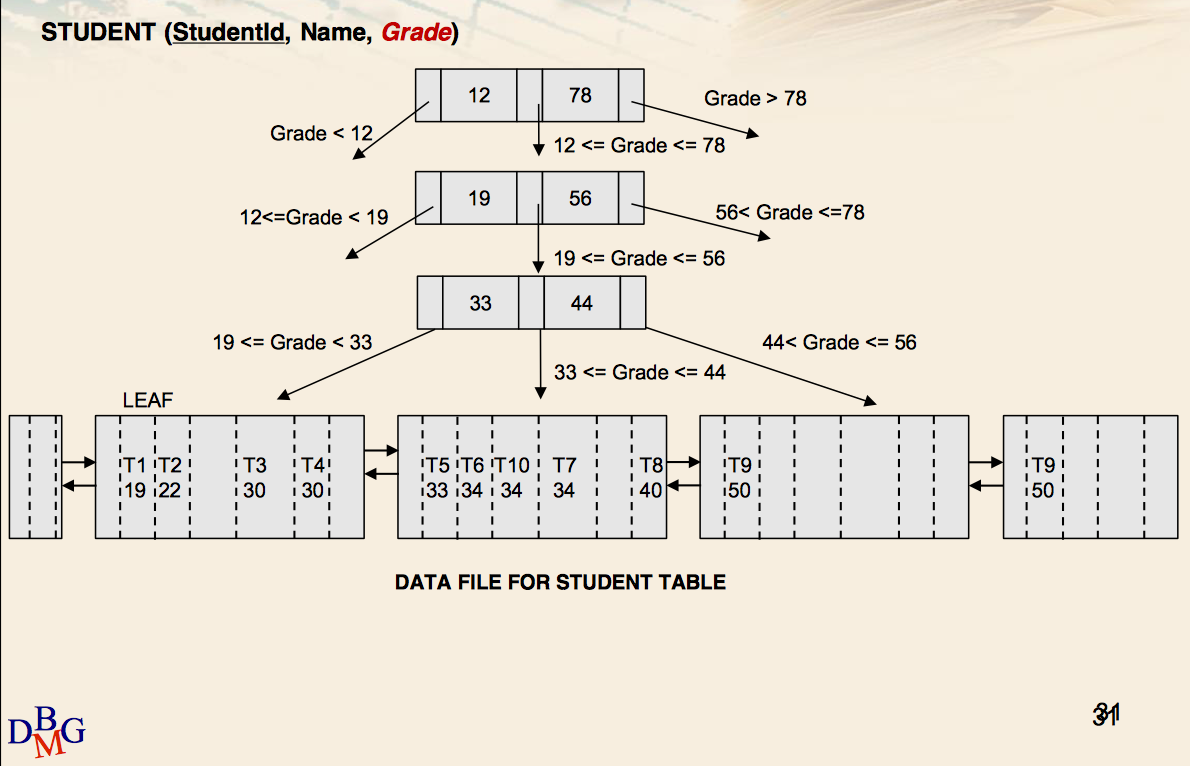
\includegraphics[width=\linewidth]{images/clu.png}
    \caption{Clustered}
    \label{fig:clu}
  \end{minipage}\hfill
  \begin{minipage}{.45\textwidth}
    \centering
    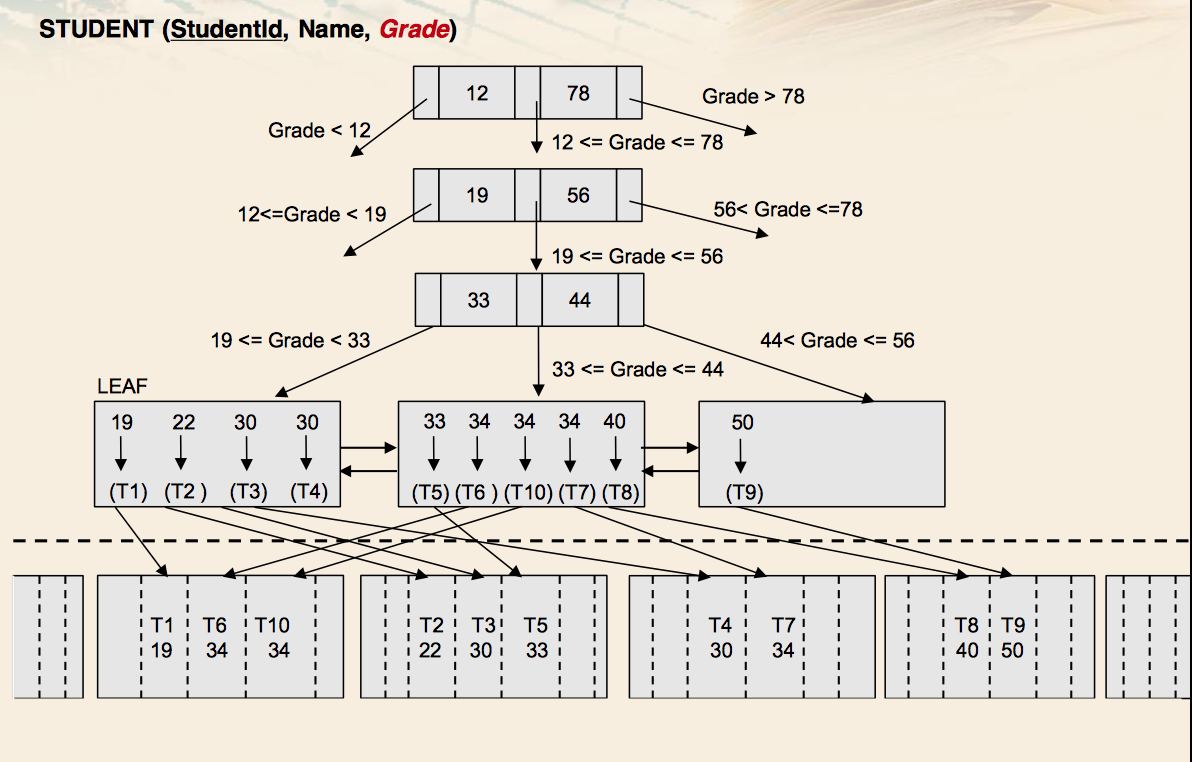
\includegraphics[width=\linewidth]{images/unclu.png}
    \caption{Unclustered}
    \label{fig:unclu}
  \end{minipage}\hfill
\end{figure}
There are two kind of B-Tree:
\begin{itemize}
  \item \textbf{B-Tree}: Data pages are reached only through key values by visiting the tree. [figure \ref{fig:b}]
  \item \textbf{$B^{+}$-Tree}: Provides link leaf allowing sequential access in the sort order. [figure \ref{fig:bplus}]
\end{itemize}
\begin{figure}[!hbpt]
  \centering
  \begin{minipage}{.45\textwidth}
    \centering
    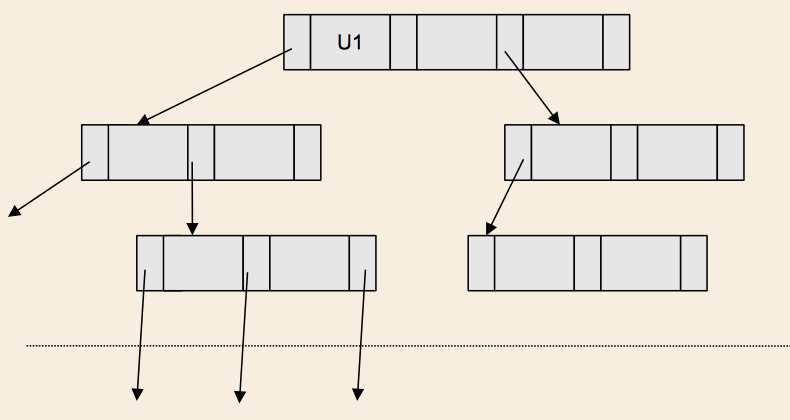
\includegraphics[width=\linewidth]{images/b.png}
    \caption{B-Tree}
    \label{fig:b}
  \end{minipage}\hfill
  \begin{minipage}{.45\textwidth}
    \centering
    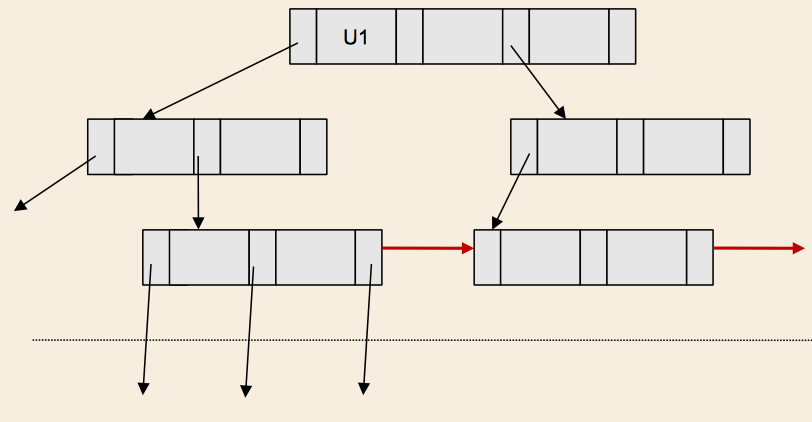
\includegraphics[width=\linewidth]{images/bplus.png}
    \caption{$B^{+}$-Tree}
    \label{fig:bplus}
  \end{minipage}\hfill
\end{figure}
the B stands for \textbf{Balanced} where leaves are all at the same distance from the root and the search time is the same indipendently by the value.\\
This structure have some:
\begin{itemize}
  \item \textbf{Advantages}:
  \begin{itemize}
    \item Very efficent for range queries.
    \item Appropriate for sequential scan in the order of the key field (always for clustered, not guarantee otherwise).
  \end{itemize}
  \item \textbf{Disadvantage}:
  \begin{itemize}
    \item Insertion may require a leaf or nodes split.
    \item Deletions may require merging uncrowded nodes and re-balancing.
  \end{itemize}
\end{itemize}

The \textbf{Hash} structure is another kind of weel-know structure is guarantees direct and efficent access to data based on the value of a key field (one or more attributes). Supposing to have B blocks in the hash structure the hash function is applied to the key value of a record and in return a values between 0 and b-1 which defines the position of the record, the idea is to not completly fill the blocks to allows new data insertion.
\begin{itemize}
  \item \textbf{Advantages}:
  \begin{itemize}
    \item Very efficent for queries with equality predicate on the key.
    \item No sorting of disk blocks is required.
  \end{itemize}
  \item \textbf{Disadvantage}:
  \begin{itemize}
    \item Inefficent for range queries.
    \item Collision may occur.
  \end{itemize}
\end{itemize}

The unclustered versione is similar to the hash index, the main difference is that the actual data is stored in a separate structure and the position of tuples is not constrained to a block.\\

The \textbf{bitmap index} is another structure that provides direct and efficient access to data based on the value of a key field, it's based on a bit matrix. The bit matrix references data rows by means of RIDs (Rows IDentifiers), the actual data is stored in a separate structure and the tuples position is not constrained.\\
The bit matrix has:
\begin{itemize}
  \item One column for each different value of the indexed attribute
  \item One row for each tuple.
\end{itemize}
the \textit{(i, j)} position has a 1 if the tuple \textit{i} as \textit{j} like attributes for the key field, 0 otherwise.
\begin{figure}[h!]
  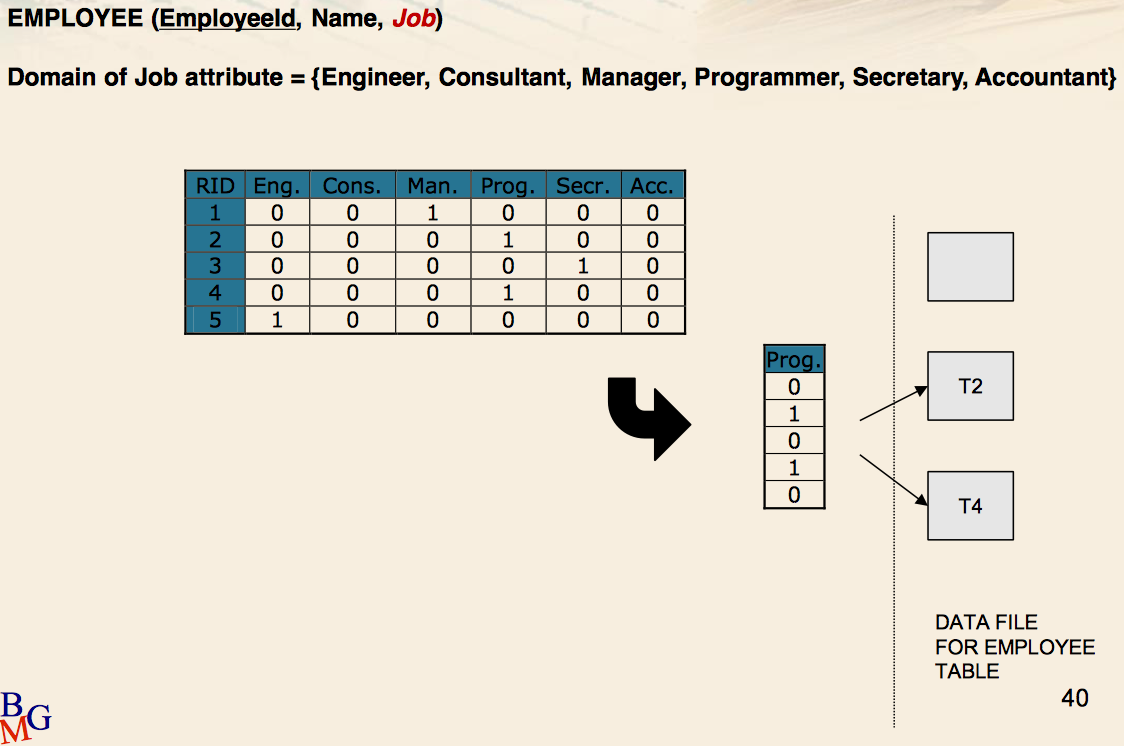
\includegraphics[width=\linewidth]{images/bitmapindex.png}
  \caption{Bitmap Index}
  \label{fig:bitmapindex}
\end{figure}
the main characteristics are:
\begin{itemize}
  \item \textbf{Advantages}:
  \begin{itemize}
    \item Very efficent for boolean expressions of predicates.
    \item Appropriate for attributes with limited domain cardinality.
  \end{itemize}
  \item \textbf{Disadvantage}:
  \begin{itemize}
    \item Not used for continuous attributes.
    \item Required space grows significantly with domain cardinality.
  \end{itemize}
\end{itemize}

\subsection{Query Optimization}
The query optimizer is part of the Optimizer and its job is selecting an efficient strategy for query execution, this block is really important. Another important task is to guarantees the data independence property, in fact, the form in which the SQL query is written does not affect the way in which it is implemented and a physical reorganization of data does not require rewriting SQL queries.\\
The query optimizer generates a \textbf{Query Execution Plan} to use the best strategies to run the query, it evaluates many different alternative, it use data statistics, use best-know strategies and it adapts automatically on data changes. The plan has more phases as you can see in figure \ref{fig:opt_plan}. The behaviour of each phase is:
\paragraph{Lexical, Synctactic and Semantic analysis}: check the SQL for Lexical errors (e.g., misspelled keywords), Syntactical errors in the SQL grammar and for Semantic erros not existing object called in the query (require data dictionary). The output of this block is an internal rappresentation of extended relational algebra because it can represent the order in which operators are applied (procedural) and there are a lot of theorems and properties.\\
\paragraph{Algebraic Optimization}: executing algebraic transformations is considered to be always beneficial, it should eliminate the difference among different formulations of the same query and is usually independet of the data distribution. The output of this phase is a "canonical" tree.\\
\paragraph{Cost Based Optimization}: This phase select the best execution plan evaluating the execution cost, it use a selection of:
\begin{itemize}
  \item Best access method for each table.
  \item Best algorithm for each relational operator among available alternatives.
\end{itemize}
the last step of this phase is the generation of the code implementing the best strategies, the output is the executable and all the dependencies used.\\
There are two types of execution modes:
\begin{itemize}
  \item \textbf{Compile and Go}: Compilation and immediate execution, no storage of query plan and no need of dependencies.
  \item \textbf{Compile and Store}: The plan is stored in the DB together with its dependencies, it's executed on demand and it need to be recompiled in data structure changes.
\end{itemize}

\begin{figure}[h!]
  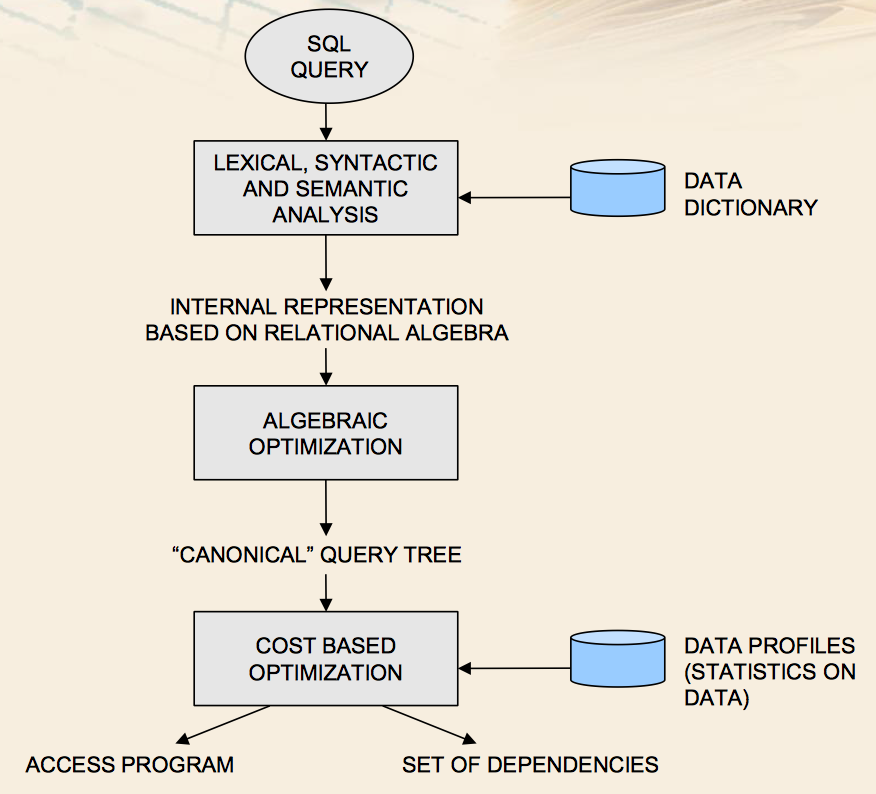
\includegraphics[width=\linewidth]{images/opt_plan.png}
  \caption{Optimization Execution Plan}
  \label{fig:opt_plan}
\end{figure}

The phase of \textbf{Algebraic Optimization} require a little more of analysis. The part is bbased on equivanlence trasformations, \textit{two relational expressions are equivalent if they both produce the same query result for any arbitrary database instance}. The main objective of this part is to \textbf{reduce the size of the intermediate result}.\\
There are some well-know transformation:
\begin{enumerate}
  \item \textbf{Atomization of selection}: Applying all attributes of selection one at a time or all together can provide different performance in case of indicies.
  \item \textbf{Cascading Projections}: It possibile to perform directly the final projection o doing more projections with different sub-set and you can obtain the same result.
  \item \textbf{Selection before join}: Anticipating the selection respect a join-operation can reduce the cardinality of the system reducing the number of operations for the join (is always used by the DBMS).
  \item \textbf{Join derivation from Cartesian Product}: Perform a cartesian product and then a selection over data get the same result as the join operation but more slowly.
  \item \textbf{Distributing selection respect union}: Is equivalent to select a sub-set and then merge it with another subset or merge the two set and then selecting it.
  \item \textbf{Distributing selection respect difference}: The formulas explain better: $\sigma_{F}(E_1 - E_2) = \sigma_{F}(E_1) - \sigma_{F}(E_2) = \sigma_{F}(E_1) - E_2 $.
  \item \textbf{Distributing projection respect union}: Projection of union of 2 table is equivalent to the union of 2 already projected table.
  \item \textbf{Other}: $\sigma_{F1 \vee F2}(E) = (\sigma_{F1}(E)) \cup (\sigma_{F2}(E))$
  \item \textbf{Other}: $\sigma_{F1 \wedge F2}(E) = (\sigma_{F1}(E)) \cap (\sigma_{F2}(E))$
  \item \textbf{Distributing join respect union}: Perform join of a table E with two merged table (E1 $\cup$ E2), is equivalent to join E with E1 and E2 separate and the merge it.
\end{enumerate}

The phase of \textbf{cost based optimization} is a little bit more complicated, it is based on:
\begin{itemize}
  \item \textbf{Data Profiles}: Statistical information describing data distribution for tables and intermediate relational expression.
  \item \textbf{Approximate cost}: Evaluating cost by looking at CPU, HDD and main memory usage and time.
\end{itemize}
The profilings of table save quantitavive information on the characteristics of tables and columns:
\begin{itemize}
  \item Cardinality of tuples.
  \item Size in bytes of tuples.
  \item Size in bytes of each attributes.
  \item Number of dinstinct values of each attribute.
  \item Min and max value of each attribute.
\end{itemize}
all this information are stored in the data dictionary that is periodically refreshed.\\

The access operators can perform different types of scans. The \textbf{sequential scan} execute sequential access to all tuples in a table (a.k.a Full Table Scan). The operation performed during a sequential scan:
\begin{itemize}
  \item Projection.
  \item Selection (Simple predicate).
  \item Sorting based on attribute list (memory sort or sort on disk).
  \item Insert, Update or Delete.
\end{itemize}
the predicate evaluation is fundamental to provide an efficent access to the data. The index access it may be exploit with all kind of structures, in case of simple equality predicate all structure are appropriate. Instead, for range predicate, the only appropriate one is the $B^{+}$-Tree. For predicates with limited selectivity full scan is better (if available bitmap could be used). In case of conjunction fo predicates the most selective one is evaluated first through the index, then the other. A possible optimization could be computing the intersection of bitmaps coming from available indices and then a table read for remaing predicates. In the disjunction the index access can be used only if all predicates have and usable index, otherwise FTS.\\

The \textbf{join} operation can be a critical operation for a relational DBMS, the connection between tables is based on values instead of pointer. There are several algorithms that can be used for the join:
\begin{itemize}
  \item \textbf{Nested Loop}: For each tuples of the outer table, the inner one is readed once. (BRUTE FROCE)
  \begin{itemize}
    \item Efficent when the inner tavle is small and fits in memory or when the join attribute in the inner table is indexed.
    \item Not cost symmertric. It depends on which table takes the role of inner.
  \end{itemize}
  \item \textbf{Merge Scan}: It sort the two tables on the join attribute and it start a parallel scan.
  \begin{itemize}
    \item Symmetric in terms of cost. Efficent for large and already-sorted tables.
    \item Requires sorting both table (already sorted or trough clustered index).
  \end{itemize}
  \item \textbf{Hash Join}: It applicate the same hash function to the join attrbute of both table. Tuples to be joined will fill the same bucket.
  \begin{itemize}
    \item Very fast join.
    \item Local sort and join is performed into each bucket.
  \end{itemize}
  \item \textbf{Bitmapped Join Index}: It precompute the join. The position (i,j) of the matrix is 1 if the tuple with RID j of A joins with tuple with RID i in table B and 0 otherwise.
  \begin{itemize}
    \item A data change need a recompute of table.
    \item Used in OLAP queries.
    \item It can exploit one or more bitmapped join indices (one for each pair of joined tables) and accessing the large central table is the last step.
  \end{itemize}
\end{itemize}

The \textbf{Group By} is one of the most important function of SQL and is performed in 2 different ways: The first one is the sort based, it sort the data on the group by attributes and the compute aggregate functions on groups; the hash based one instead it perform and hash function over data, sort the bucket just created and than compute the aggregate function.

\paragraph{Execution plan selection} is based on some data input, the data profiles (statistics over data) and the internal representation of the query tree, the output of this part is the "optimal" (it can't assure that it will be the best one) execution plan. This phase evaluate the cost of different alternatives for read tables and executing each relational operator exploting an approximate cost of execution.\\
The search is based on the following parameters:
\begin{itemize}
  \item Scan type of data (full scan, index).
  \item Execution order among operators.
  \item Type of operators implementation (different join methods).
  \item Sorting time (when).
\end{itemize}
The approach work on a tree of alternatives where each nodes represent a decision on a variable and the leaf one complete query execution plan. Of course the system select the cheapest one. The general formula is $C_{Total} = C_{I/O}*n_{I/O} + C_{CPU}*n_{CPU}$ where $n_{I/O}$ is the number of I/O operations and $n_{CPU}$ is the number of CPU operations.\\
The final plan is an approximation of the best solution. Th optimizer looks for a solution which is of the same order of magnitude of the "best" solution. In the \textbf{Compile and Go} execution mode the search is stopped when the time spend for the search is comparable to the time required to execute the current best plan. % 4_QueryOptimization finished

\subsection{Physical Design}
The physical distribution of the data in the system is fundamental for providing good performance. Taking in account the logical schema of the DB, the features of the selected DBMS and thw workload this block provides a physical schema of the databse (table organization, indices) and all necessary set up parameters for storage and configurations.\\
The possible physical file organization are:
\begin{itemize}
  \item Unordered (heap).
  \item Ordered (clustered).
  \item Hashing on hash-key.
  \item Clustering several relations.
\end{itemize}
The number of indicies is related to the structure type of the system. In case of clustered is possible to define only one index, instead, unclustered structures allow to define multiple different indices.\\
The workload distribution is different in case of a normal query or for an update. The first case involve:
\begin{itemize}
  \item Accessed tables.
  \item Visualized Attributes.
  \item Attributes involve in selections and joins.
  \item Selectivity of selections.
\end{itemize}
the update case instead:
\begin{itemize}
  \item Attributes and tables involved in selections.
  \item Selectivity of selections.
  \item Update type (Ins/Del/Up) and updated attributes.
\end{itemize}
The selection of the structure is important and it could be changed during the usage of the system for improvement (database tuning). Changes in the logical schema are allowed and they can or cannot preserve the BCNF (Boyce Code Normal Form). There isn't a general methodology the best solutions are trial and error, some general criteria and "common sense" heuristic.\\
Some general criteria could be:
\begin{itemize}
  \item Primary Key is usually exploited for selection and joins, indexing it could be useful.
  \item Adding new indices for most common query predicates. Evaluate the actual plan and verify the improvement if available.
  \item Never index small table, the entire table requires few disk reads.
  \item Never index attributes with low cardinality (e.g. gender). This is not true for data warehouses.
\end{itemize}
from the heuristics point of view there are severals "common sense" ideas:
\begin{itemize}
  \item For attributes involved in simple predicates of where clause equality:hash and range:$B^{+}$-Tree.
  \item Evaluated clustered improvement for slow queries.
  \item For where clauses involving many simple predicates use multi attributes index or appropriate key order.
  \item Maintenance cost.
  \item To improve joins use index on inner table in case of nested loop or $B^{+}$-Tree, for merge scan, on the join attribute.
  \item For group by hash index or $B^{+}$-Tree.
  \item Consider group by push down that anticipate the group respect to joins.
\end{itemize}
of course after all the changes a good choice could be update database statistics, for future improvements the database tuning could help. The last chance can be affecting optimizer decision, the main problem is the lost of data independence.

\subsection{Concurrency Control}
The workload of operational DBMS is measured in \textit{transaction per second} (banking and flight reservation are on 10-1000 tps). This block provide concurrent access to data maximizing the throughput and minimizing response time. The elementary operations are of course \textbf{READ r(x)} and \textbf{WRITE w(x)}. The block that manage the concurrency is called scheduler is in charge of deciding if and when read/write request can be satisfied.\\
The most common anomalies are:
\begin{itemize}
  \item \textbf{Lost Update}: It occur when a tr2 read a value that is already under operations by another tr. (figure \ref{fig:lost_update})
  \item \textbf{Dirty Read}: When a tr2 read the value of x in an intermediate state which never become permanent. (figure \ref{fig:dirty_read})
  \item \textbf{Inconsistent Read}: When a tr1 read multiples times x with different value each time. (figure \ref{fig:inco_read})
  \item \textbf{Ghost Update}: It occur when two transaction are working over multiple data at the same time performing read and write. (figure )
\end{itemize}

\begin{figure}[h!]
  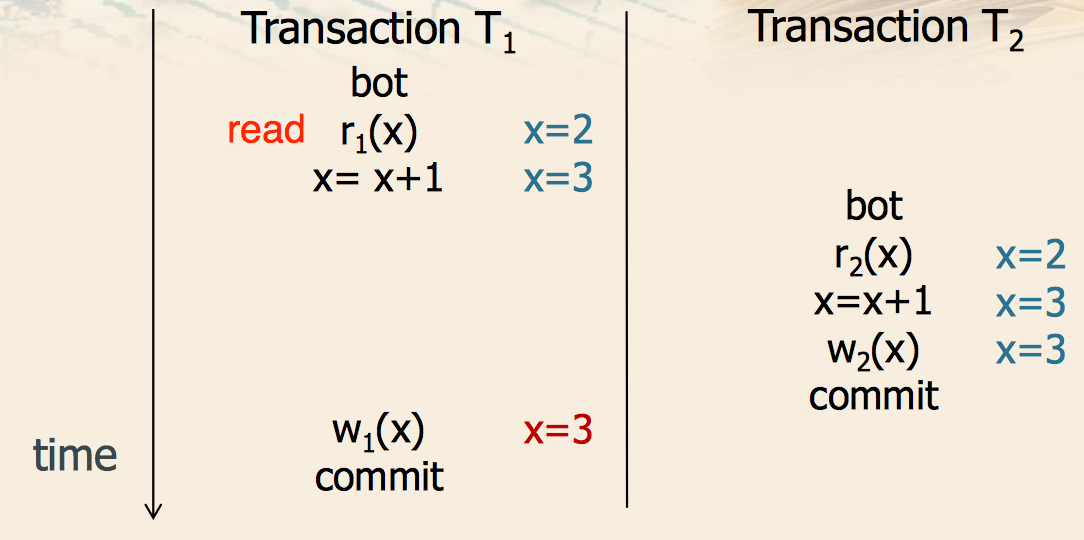
\includegraphics[width=\linewidth]{images/lost_update.png}
  \caption{Lost Update Behaviour}
  \label{fig:lost_update}
\end{figure}
\begin{figure}[h!]
  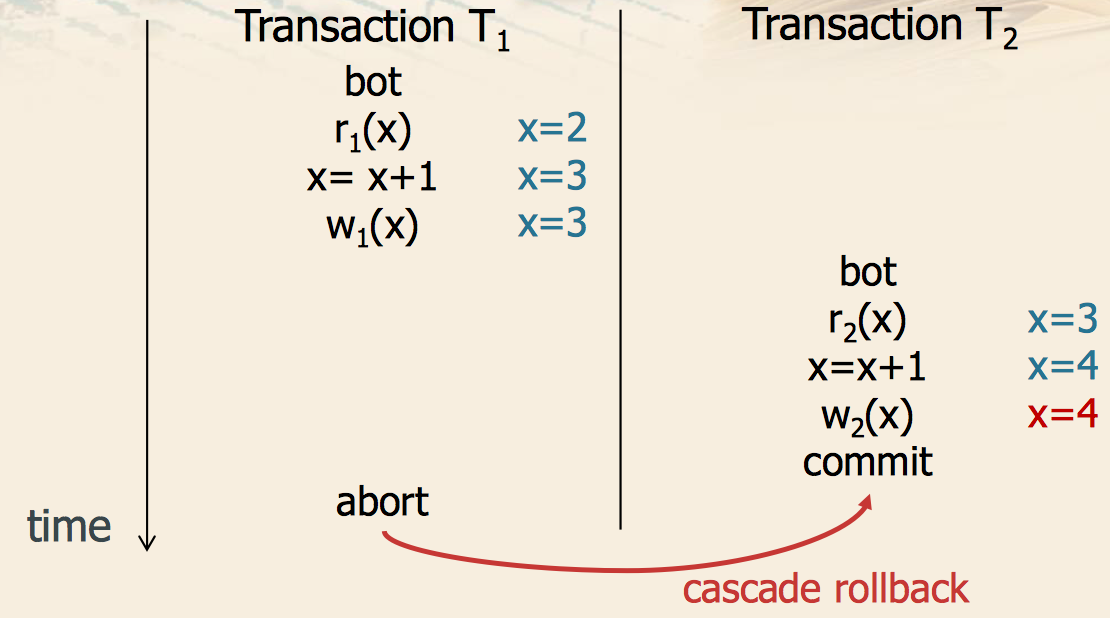
\includegraphics[width=\linewidth]{images/dirty_read.png}
  \caption{Dirty Read Behaviour}
  \label{fig:dirty_read}
\end{figure}
\begin{figure}[h!]
  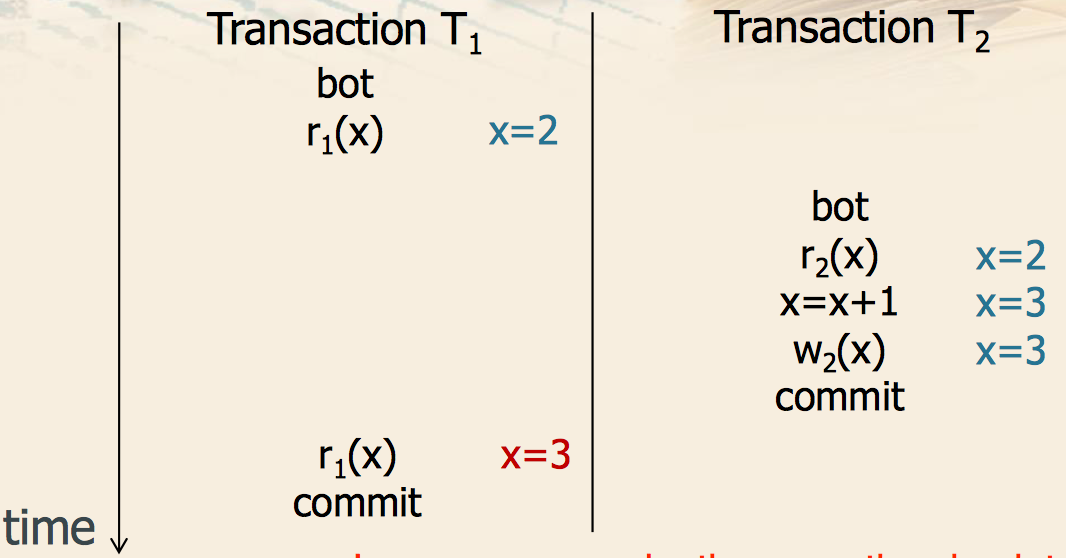
\includegraphics[width=\linewidth]{images/inco_read.png}
  \caption{Inconsistent Read Behaviour}
  \label{fig:inco_read}
\end{figure}
\begin{figure}[h!]
  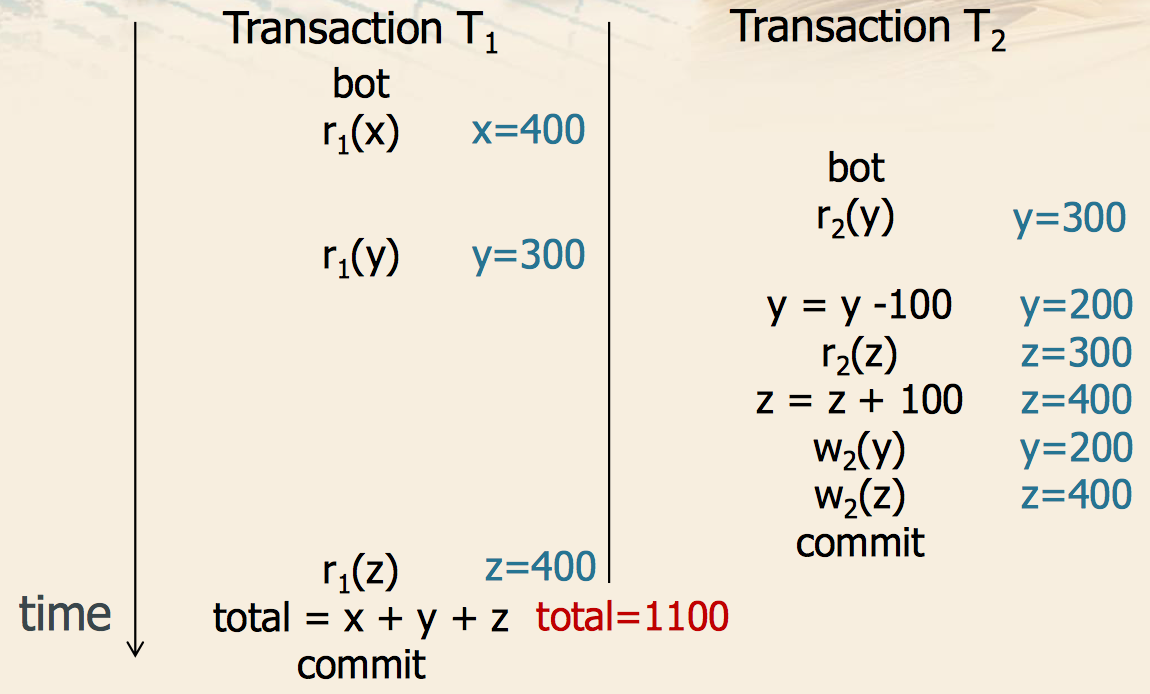
\includegraphics[width=\linewidth]{images/ghost_up.png}
  \caption{Ghost Update Behaviour}
  \label{fig:ghost_up}
\end{figure}

\paragraph{Theory of Control} a \textit{transaction} is a sequence of R/W operations with the same TID (\textit{Transaction Identifier}); the \textit{schedule} is a sequence of read/write operations presented by concurrent transaction. The scheduler is in charge of accepts or reject the requests to avoid anomalies without knowing the outcome (commit/abort) of it.\\
Commit projection is a simplifying hypothesis (the schedule only contains transaction performing commit), it avoid dirty read anomaly, it will be removed later.\\
In a \textbf{serial schedule}, the actions of each transaction appear in sequence, without interleaved actions. An arbitrary schedule $S_{i}$ is correct when it yields the same results as an arbitrary serial schedule $S_{j}$ of the same transactions. $S_{i}$ is serializable, is equivalent to an arbitrary serial schedule of the same transaction. There are different equivalence classes between two schedules:
\begin{itemize}
  \item View equivalence
  \item Conflict equivalence
  \item 2 phase locking
  \item Timestamp equivalence
\end{itemize}
each equivalence class find a set of acceptable schedules characterized by a different complexity.

\paragraph{View equivalence} there some definitions to be introduced:
\begin{itemize}
  \item \textbf{reads-from}: $r_{i}(x)$ reads-from $w_{j}(x)$ when:
  \begin{itemize}
    \item $w_{j}(x)$ precedes $r_{i}(x)$ and $i \neq j$
    \item There is no other $w_{k}(x)$ between them.
  \end{itemize}
  \item \textbf{final write}: is a final write if it is the last write of x appearing in the schedule.
\end{itemize}
with this solution two schedules are view equivalent if they have the same reads-from set or the same final write set.\\
This techniques is easy to be understand using an example. Using the flow in figure \refeq{fig:ex1}.
\begin{figure}[h!]
  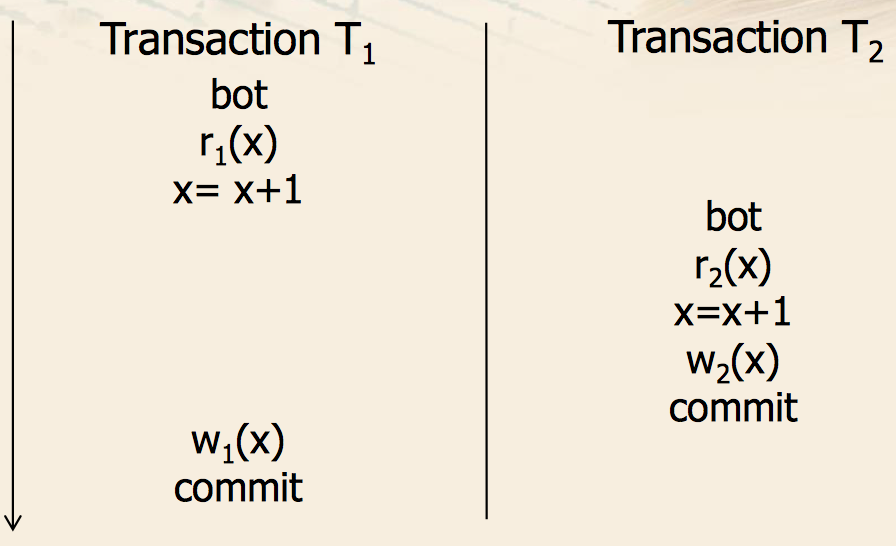
\includegraphics[width=\linewidth]{images/ex1.png}
  \caption{View Equivalence Example}
  \label{fig:ex1}
\end{figure}
The corrisponding schedule is: $S = r_{1}(x)r_{2}(x)w_{2}(x)w_{1}(x)$ is this schedule serializable?\\
There are only 2 possible serial schedules:
\begin{equation}
  \begin{gathered}
    S_{1} = r_{1}(x)w_{1}(x)r_{2}(x)w_{2}(x)\\
    S_{2} = r_{2}(x)w_{2}(x)r_{1}(x)w_{1}(x)
  \end{gathered}
\end{equation}
In both cases S is not view equivalent to any serial schedule, not serializable, should be rejected.\\
The analization of this problem is linear if the schedule is given, in case of an arbitrary schedule it become NP-complete. For this problem is better to use a less accurate, but faster techniques.

% Concurrency @ Pag. 30
\paragraph{Conflict equivalence}
Two actions are in conflict when both operate on the same object and at least one of them is a write. The conflict can be, RW, WR or WW. The conflict are equivalent if they have:
\begin{itemize}
  \item Same conflict set.
  \item Each conflict pair is in the same order in both schedules.
\end{itemize}
A schedule is conflict serializable (\textbf{CSR}) if it is equivalent to an arbitrary serial schedule of the same transaction.\\
Dectecting the conflict serializability it is possible to exploit the conflict graph:
\begin{itemize}
  \item Node: Each transaction.
  \item Edge i$\rightarrow$j: if is there at least a conflict between $T_{i}$ and $T_{j}$.
\end{itemize}
checking the cyclicity of a graph is linear in the size of the graph.

\paragraph{2 Phase Locking} a lock is block on a resource which may prevent access to others. The operations are:
\begin{itemize}
  \item \textbf{Lock}
  \begin{itemize}
    \item Read Lock (R-Lock)
    \item Write Lock (W-Lock)
  \end{itemize}
  \item \textbf{Unlock}
\end{itemize}
Each operation is preceded by a request of R/W-Lock and is followed by a request of unlock. Of course the R-Lock is shared among different transaction, the write lock instead is exclusive, not compatible with any other lock.\\
The scheduler becomes a lock manager it receives transaction requests and grants locks based on locks already granted and so on...\\
When the lock request id \textbf{granted}:
\begin{itemize}
  \item The resource is acquired by the requesting transaction.
  \item After the unlock, the resource, becomes again available.
\end{itemize}
When the lock is \textbf{not granted}:
\begin{itemize}
  \item The requesting transaction is put in a waiting state.
  \item The wait is terminated when the resources is unlocked and becomes available again.
\end{itemize}
All the information for grant or not the lock are stored in the \textbf{lock table} with the \textbf{conflict table} (figure \ref{fig:conflict}) used to manage lock conflicts.

\begin{figure}[h!]
  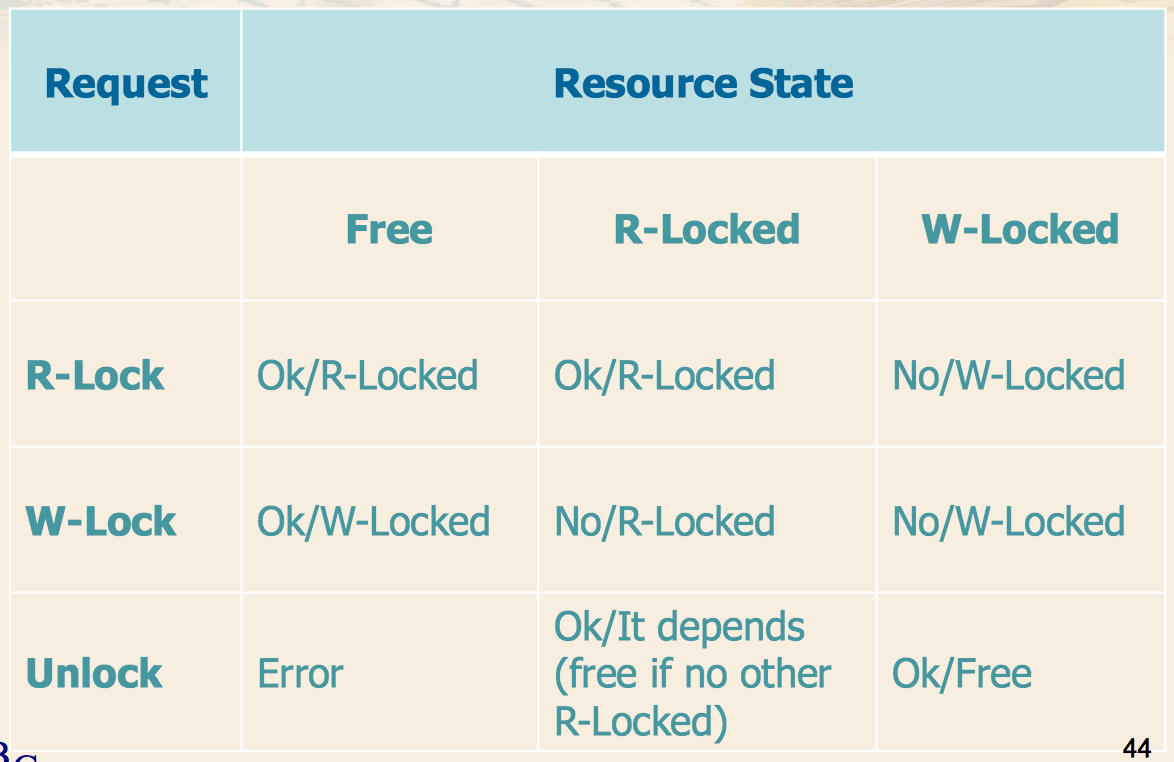
\includegraphics[width=\linewidth]{images/conflict.png}
  \caption{Conflict Table}
  \label{fig:conflict}
\end{figure}

The read locks are shared this is because the read not change the state of a data and multiple access can be exploited at the same time. A counter is used to count the number of R-Lock granted on a resources.\\
The lock manager, that coordinates the grant, exploit the lock table stored in main memory and, for each data object, use 2 bits to represent the 3 possible states (free, r-locked, w-locked) and a counter to count the number of waiting transaction. An example in figure \ref{fig:TwoPhaseEx}.

\begin{figure}[h!]
  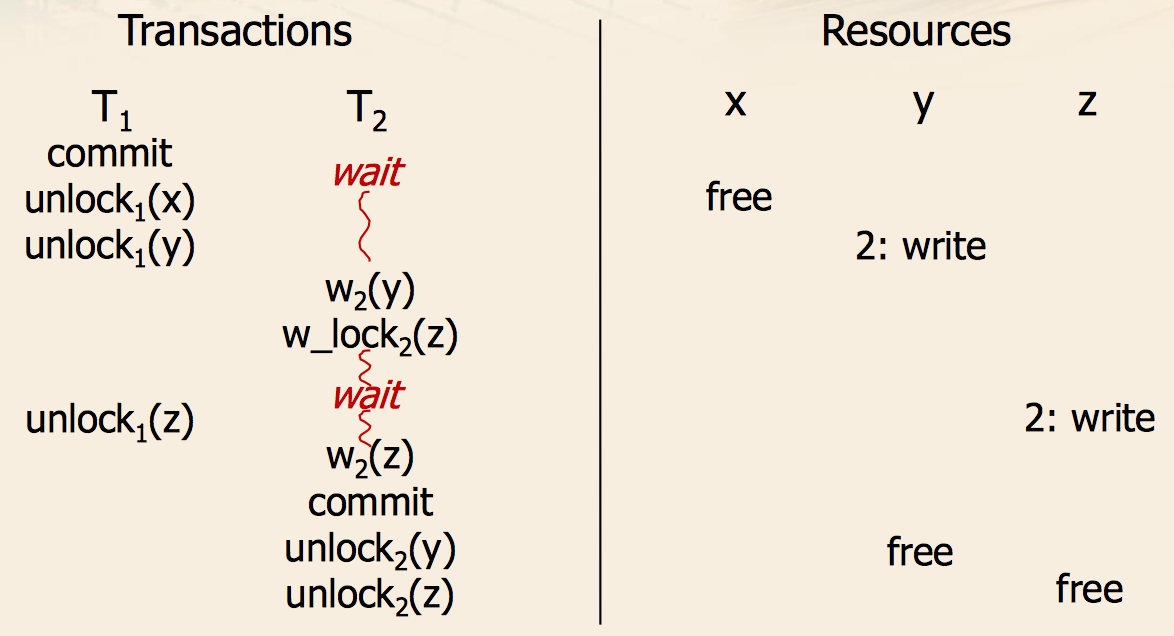
\includegraphics[width=\linewidth]{images/TwoPhaseEx.png}
  \caption{Conflict Table}
  \label{fig:TwoPhaseEx}
\end{figure}

There is also another version of the 2 phase locking the STRICT version. In this solution the unlock will be performed only at the end o the transaction and not when the resources is released; this difference guarantee to avoid the dirty read anomaly.\\
The procedure is really fast. If a transaction keep in wait over timeout the lock manager resume it and returns a NOT OK ERROR, the requesting transaction may perform a rollback o request again the same resources.

% Concurrency Control @ Pag. 57 = Hierarchical Locking
\paragraph{Hierarchical Locking} locks tables at different granularity levels:
\begin{itemize}
  \item Table
  \item Group of Tuples (fragment)
  \item Single Tuple
  \item Single Field in a Tuple
\end{itemize}
this is an extension of the traditional locking. It allows a transaction to request a lock at the appropriate level of the hierarchy and it is characterized by a large set of locking primitives.\\
The \textbf{Locking Primitives} are:
\begin{itemize}
  \item \textbf{Shared Lock (SL)}
  \item \textbf{eXclusive Lock (XL)}
  \item \textbf{Intention of Shared Lock (ISL)}: It shows the intention of shared locking on an object which is in a lower node in the hierarchy.
  \item \textbf{Intention of eXclusive Lock (IXL)}: Similar to ISL, but for exclusive lock.
  \item \textbf{Shared lock and Intetion of eXclusive Lock (SIXL)}: Shared lock of the current object and intention of exclusive lock for one or more objects in a descandant node.
\end{itemize}
The behavior is reported in figure \ref{fig:hierlock}.
\begin{figure}[h!]
  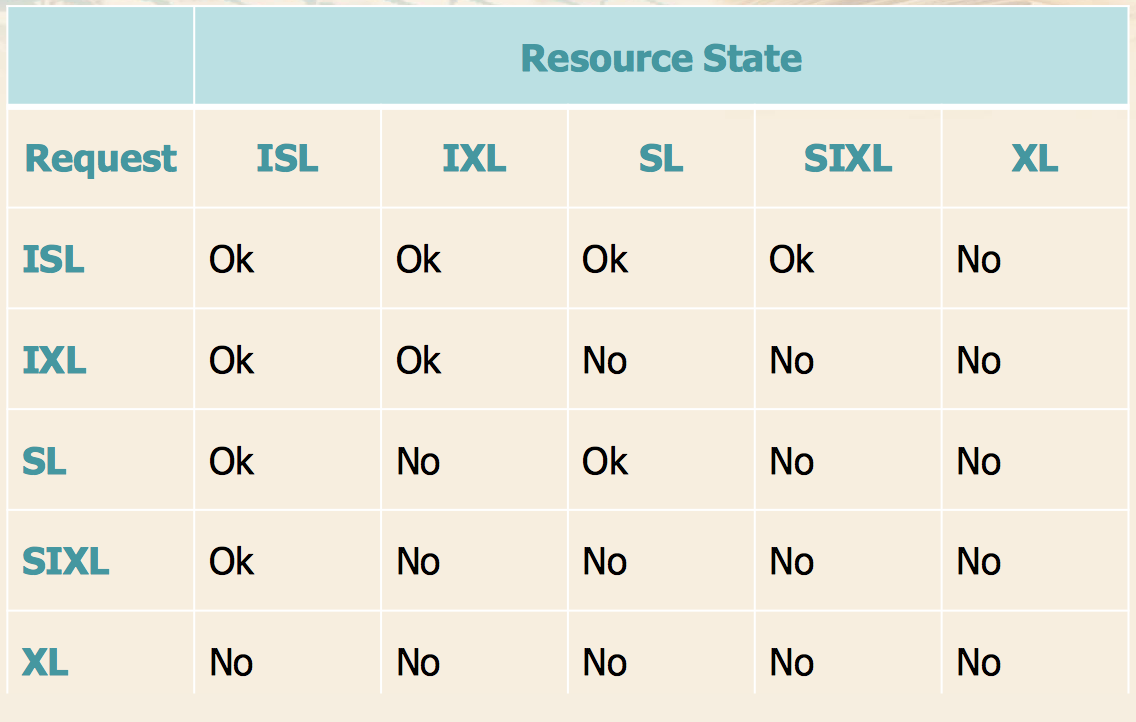
\includegraphics[width=\linewidth]{images/hierlock.png}
  \caption{Hierarchical Behavior}
  \label{fig:hierlock}
\end{figure}

The selection of lock granularity depends on the application type:
\begin{itemize}
  \item If it performs localized reads or updates of few objects (low lv - detailed ganularity).
  \item If it performs massive reads or updates (high lv - rough granularity).
\end{itemize}
the effect of lock granularity:
\begin{itemize}
  \item If it is too coarse, reduces concurrency.
  \item If it is too fine, it forces significant overhead on the lock manager.
\end{itemize}

The predicate locking addresses the ghost update of type b (insert) anomaly, for the 2PL a read operation is not in conflict with the insert of new tuple, they can't be locked in advance. The PredLock allows locking all data satisfying a given predicate.

There are several isolation level:
\begin{itemize}
  \item \textbf{SERIALIZABLE}:
  \begin{itemize}
    \item Highest
    \item PredLocking
  \end{itemize}
  \item \textbf{REPEATABLE READ}:
  \begin{itemize}
    \item Strict 2PL without PredLock
    \item Read existing obj can be correctly repeated
    \item No protection ghost update
  \end{itemize}
  \item \textbf{READ COMMITTED}:
  \begin{itemize}
    \item Not 2PL
    \item The read lock is released as soon as the object is read
    \item Reading intermediate states of a transaction is avoided (dirty reads)
  \end{itemize}
  \item \textbf{READ UNCOMMITTED}:
  \begin{itemize}
    \item Not 2PL
    \item Data reads without acquiring the lock
    \item Only allowed for read only transaction
  \end{itemize}
\end{itemize}

\textbf{Deadlocks} can be frequent, the solution for solving it are implementing \textbf{timeout} the transaction waits for a given time, after the expiration of TO it receives a negative answer and it performs rollback. The time length could be LONG and SHORT (can be overloads the system). Other solution can be performed Pessimistic 2PL that acquire all locks before the transactions start (not always feasible) or the timestamp that put in wait mode only younger transaction. The deadlocks detection is performed using the wait graph, it could be expensive to build and mantain.

\subsection{Reliability Management}
It is responsible of the atomicity and durability ACID properties, it implements the following transactional commands:
\begin{itemize}
  \item BEGIN transaction (B)
  \item COMMIT (C)
  \item ROLLBACK (A, for Abort)
\end{itemize}
it also provides recovery primitives WARM and COLD RESTART.\\
It manages the reliability of R/W requests by interacting with the buffer manager, it may generate new R/W requests for reliability purposes. It exploits the \textbf{log file} a persistent archive recording DBMS activity and is stored in a "stable" memory (not affected by failure, abstraction). It prepares data for performing recovery by means of the operations \textit{checkpoint} and \textit{dump}.\\
\paragraph{Log file} is a sequential file written in stable memory that records transaction activities in chronological order. The record can be related to a transaction or system, they are saved interleaved between different transaction.\\
The transaction log are written in this way:
\begin{itemize}
  \item BEGIN B(T)
  \item COMMIT C(T)
  \item ABORT A(T)
  \item INSERT I(T, O, AS)
  \item DELETE D(T, O, BS)
  \item UPDATE U(T, O, BS, AS)
\end{itemize}
where O represent the written object, AS is the After State (state of object O after modification) and BS is the Before State.\\

\textbf{Checkpoint} are periodically operation requested by the RM to the BM, it allows a faster recovery process. During the checkpoint, the DBMS writes data on disk for all completed transactions.\\
The flow of the checkpoint is:
\begin{enumerate}
  \item All the TIDs of all active transaction are recorded
  \begin{itemize}
    \item After the checkpoint start, no transaction can commit until the checkpoint ends.
  \end{itemize}
  \item The pages of concluded (C or A) transaction are synchronously written on disk.
  \begin{itemize}
    \item By means of the froce primitive.
  \end{itemize}
  \item A the end of step 2, a chekcpoint record is synchronously written on the log.
  \begin{itemize}
    \item Contains the set of active transactions.
    \item It is written by means of the focre primitive.
  \end{itemize}
\end{enumerate}

\textbf{Dump} is a complete copy of the database, typically performed when the system is offline, stored in stabel memory, may be incremental. At the end a dump record is written in the log.\\

The log is designed to allow recovery in presence of failure, WAL or Commit precedence. The WAL (Write Ahead Log, SYNC) the BS of data in a log record is written in stable memory vefore database data is written on disk, during recovery it will allows UNDO operation. The COMMIT PRECEDENCE (ASYNC) solution write the AS in a stable memory before commit, this will allows the execution of redo operations.\\

\paragraph{Recovery Management} there are two types of failures, the SYSTEM caused by software problem or power supply interruption that are causing losing in the main memoery content (buffer) but not on the disk. Or the MEDIA failure, caused by failure of devices managing secondary memory, this will lose the DB content on disk but not the log.\\
When a failure occurs the system is stopped, the type of recovery to be started depends on the failure type: SYS=WARM and MEDIA=COLD. When the recovery ends the system becomes again available to transactions.\\
The \textbf{WARM RESTART} is one of the solution for the recovery procedure:
\begin{itemize}
  \item All the transaction completed before the checkpoint not need a recovery action.
  \item The transaction which committed, but for which some write on disk are not already performed REDO is needed.
  \item Active transaction at the time of failure (not committed) UNDO is needed.
\end{itemize}
the checkpoint is not needed to enable recovery, it only provides faster restart, because, without it, the entire log until the last dump needs to be read. This solution reads backwards the log to detecs action which should be undo or redo, then star to read forward the log and perform all the actions.\\
The \textbf{COLD RESTART} is the second solution for recovery, it is performed when a portion of the database on disk get a failure. The main steps are:
\begin{enumerate}
  \item Access the last dump to restore the damaged portion of the DB on disk.
  \item Starting from the last dump record, read the log forward and redo all actions on the database and transaction commit/rollback.
  \item Perform a warm restart.
\end{enumerate}

\subsection{Triggers}
The traditional DBMS is passive, query and updates are explicitly requested by users, the knowledge of processes operating on data is typically embedded into applications. The active DBMS instead have a Reactivity service provided that monitors specific database vents and triggers actions in response. Reactivity is provided by automatically executing rules, they can be:
\begin{itemize}
  \item Event: Modification operation.
  \item Condition: Predicate on the DB state, cond==true: action==execute.
  \item Action: Sequence of SQL instructions or application procedure.
\end{itemize}
The rule engine is the component in charge of tracking events and executing rules when appropriate. The execution of the rules is interleaved with traditional transactions.\\
SQL provides instructions for defining triggers (CREATE TRIGGER) the syntax and semantics are covered in the SQL3 standard. The structure is divided in 3 main part:
\begin{itemize}
  \item WHEN: the events takes place.
  \item IF: the condition is true.
  \item THEN: the action is executed.
\end{itemize}
there are also some execution modes:
\begin{itemize}
  \item Immediate: before or after the triggering statement.
  \item Deferred: executed immediately before commit. (Not commercial)
\end{itemize}
and the granularity:
\begin{itemize}
  \item Tuple (or row level): One separate exec of the trigger \textit{for each tuple} affected by the triggering statement.
  \item Statement: One single trigger execution \textit{for all tuples} affected by the triggering statement.
\end{itemize}

\paragraph{Oracle Triggers} % Triggers @ Pag. 17 - Oracle Triggers
The base structure of a trigger is:

\begin{lstlisting}[frame=single]
  CREATE TRIGGER TriggerName
  Mode Event {OR Event }
  ON TargetTable
  [[ REFERENCING ReferenceName]
  FOR EACH ROW
  [WHEN Predicate]]
  PL/SQL Block
\end{lstlisting}
It can be divided in:
\begin{itemize}
  \item Mode is BEFORE or AFTER
  \item Event ON TargetTable is:
  \begin{itemize}
    \item INSERT
    \item DELETE
    \item UPDATE
  \end{itemize}
  \item FOR EACH ROW specifies row level execution semantics.
  \begin{itemize}
    \item OLD.ColName and NEW.ColName are used for accessing to the two types of data.
  \end{itemize}
  \item WHEN is used only for row level execution.
\end{itemize}

The execution algorithm is:
\begin{enumerate}
  \item Before statement triggers are executed.
  \item For each tuple in \textit{TargetTable} affected by the triggering statement.
  \begin{enumerate}
    \item Before row triggers are executed.
    \item The triggering statement is executed + Integrity constraints are checked on Tuples.
    \item After row triggers are executed.
  \end{enumerate}
  \item Integrity constraints on tables are checked.
  \item After statement triggers are executed.
\end{enumerate}
the execution order for triggers with the same event, mode and granularity is not specified and it could be source of non determinism. If an error occurs the roll back of the triggers operation is performed. The triggers could also called in cascade, the maximum is defined by the user. The \textit{mutating table} is the table modified by the statement triggering the trigger. The MT cannot be accessed in row level triggers, may only be accessed in statement triggers (limited access only on Oracle application).

\subsection{Distributed Architectures}
A possible architectural implementations is using a distributed system, the main advantages are related to performance improvement, increased availability and stronger reliability. Of course the classic client/server mechanicsm is much easier to be implemented and mantained. The distributed one are able to collaborate and are autonomous, the only problem is to guaranteeing the ACID property that requires more complex techniques.\\
\paragraph{Client/Server} there are two main types of structure, the first is the \textbf{2-TIER}:
\begin{itemize}
  \item \textit{n} clients: With some application logic.
  \item DBMS Server: Provides access to data.
\end{itemize}
the \textbf{3-TIER} solution istead:
\begin{itemize}
  \item \textit{n} clients: Browser.
  \item Application server: Business logic and also web server.
  \item DBMS Server: Provides access to data.
\end{itemize}

\paragraph{Distributed} system are accessed by many user at the time. Each user can be also access more than one DBMS server. Each server need to have a local autonomy, each manages its local data, concurrency control, recovery, etc... The localization instead could be the most important difference respect c/s system, this can perform a geographical distribution. Also the data availability, less probability off total block, but more in terms of local block. Least but not last, the scalability.

\paragraph{Design} given a relation R, a data fragment is a subset of R in terms of
\begin{itemize}
  \item Tuples:Horizontal = Not overlapped, union of table possible.
  \item Schema:Vertical = Overlapped on PK, join of table.
  \item Both:Mixed
\end{itemize}
The distributed system are based on data fragmentation over different servers. THe allocation schema describes how fragments are stored on different server nodes, it could be redundant or not redundatan if some fragments are replicated or not on different servers. When there are replication the data availability increase, but also the complexity, synchronization is needed.\\
The trasparency levels explains how data distribution are visible by the query programmer, the could be invisible, in this case programmer will call only one table without knowing the fragment division. Another option is knowing the existence of fragments but not their allocation, in this case each fragment not to be used like a different table.

\paragraph{Classification} the client is only responsible to request the execution of the query, the taks to redistributing the computation is demanded to the DBMS server. The transaction could be classificated:
\begin{itemize}
  \item \textbf{Remote Request}:
  \begin{itemize}
    \item Read only request
    \item Single remote server
  \end{itemize}
  \item \textbf{Remote Transaction}:
  \begin{itemize}
    \item Any SQL command
    \item Single remote server
  \end{itemize}
  \item \textbf{Distributed Transaction}:
  \begin{itemize}
    \item Any SQL command
    \item Each SQL statement is addressed to one single server
    \item Global atomicity is needed
  \end{itemize}
  \item \textbf{Distributed Request}:
  \begin{itemize}
    \item Each SQL command may refer to data on different servers
    \item Distributed optimization is needed
    \item Fragmentation transparency is in this class only
  \end{itemize}
\end{itemize}

\paragraph{Technology} using more system requires synchronization. To guarantee the ACID property some techniques need to be implemented:
\begin{itemize}
  \item Atomicity: 2 phase commit.
  \item Consistency: Enforced only locally.
  \item Isolation: Strict 2PL and 2 Phase Commit.
  \item Durability: Extension of local procedures to manage atomicity in case of failure.
\end{itemize}
The Distributed Query Optimization have the tasks to split in different sub-queries a single query execution request. After fast execution plan definition, the DBMS, start the different operations and coordinates everything fot a correct information exchange.\\
The \textbf{2-Phase Commit} protocol has the objective to coordinate the conclusion of a distributed transaction. The behaviour is similar to a wedding. There is one coordinator, the Transaction Manager (like priest) and several DBMS servers which take part to the transaction, Resource Manager (like the couple). There also 2 new logs, the TM add some information related to the protocol start/end, the RM add the ready log to synchronize the commit with the other system. The procedure is similar to the window-networks protocol, with packets and ack. Figure \ref{fig:2pc} schematize the flow.

\begin{figure}[h!]
  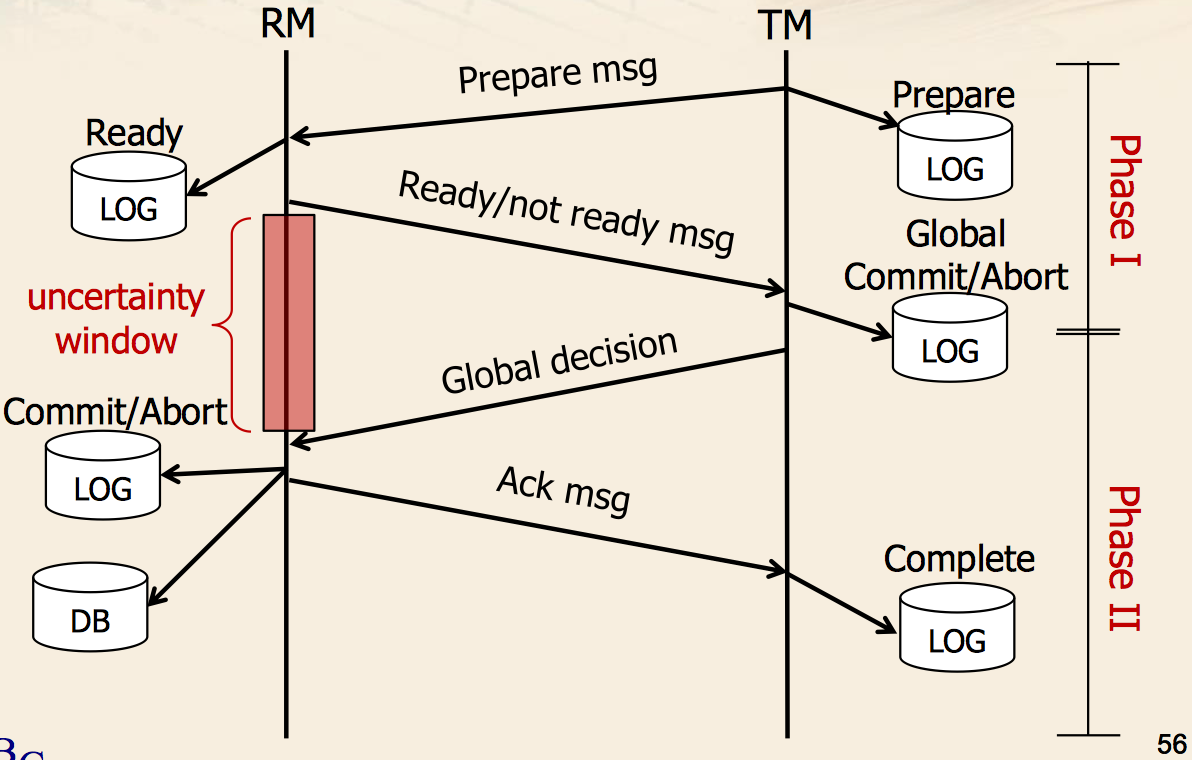
\includegraphics[width=\linewidth]{images/2pc.png}
  \caption{2-Phase Commit}
  \label{fig:2pc}
\end{figure}

The 2 phases of the coordinator are:
\begin{itemize}
  \item \textbf{I Phase}:
  \begin{itemize}
    \item Prepare (Outgoing)
    \item Ready (Incoming)
  \end{itemize}
  \item \textbf{II Phase}:
  \begin{itemize}
    \item Global Decision (Outgoing)
  \end{itemize}
\end{itemize}

Also the recovery phase is a little bit modififed, the warm restart will read the READY log and asked to the TM how to procede to the restore (Remote Recovery Request). In case of the failure of the coordinator:
\begin{itemize}
  \item Last Record=PREPARE: A global abort is written in log and send to all partecipants.
  \item Last Record=GLOBAL DECISION: Repeat the phase II.
\end{itemize}

%--------------------------------------------------------------------------------------------------------
%--------------------------------------------------------------------------------------------------------
%--------------------------------------------------------------------------------------------------------
\clearpage
\section{Data Warehouses}
\subsection{Introduction}
The database was delevoped for giving a service to the final users, like university, flight companies and other stuff. During the 80's they have understand that this system could be also used for made analisys over data. This analisys could be usefull for improving decision, forecast, cost reduction and other stuff.\\
The goal of Business Intelligence is to provides support to strategic decision, trasforming company data inyo actionable information. This request requires of course an appropriate hardware and software infrastructure.\\
The data ware house is a database devoted to decision support, which is kept separated from company operational databases. The data which is:
\begin{itemize}
  \item Devoted to specific subject
  \item Integrated and Inconsistent
  \item \textbf{Time Dependent}, non volatile
\end{itemize}
all data related to the timestamp are bigger than the other.\\
The data are kept separated for multiple questions:
\begin{itemize}
  \item \textbf{Performance}: Complex queries reduce performance. Data may varies during operation, etc... The system could be developed for doing some operations but the warehousing use the system in a different way.
  \item \textbf{Data Management}: The data for the service could be different from the data needed for the analytics. (ex. Data addresses changing). There could be also inconsistency problem.
\end{itemize}
One of the rappresentation solution proposed is the (hyper)cube with three or more dimensions (figure \ref{fig:hypercube}).
\begin{figure}[h!]
  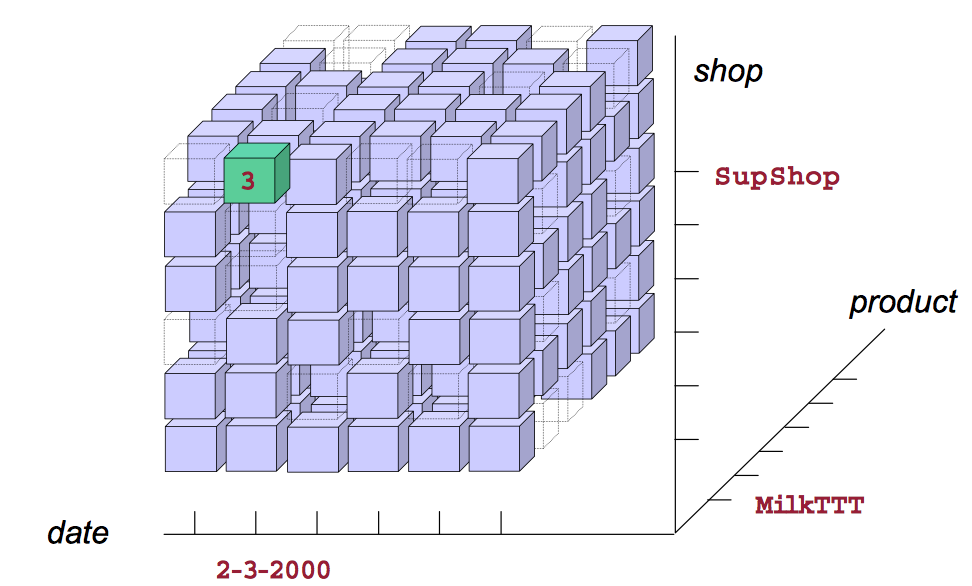
\includegraphics[width=\linewidth]{images/hypercube.png}
  \caption{Hypercube rappresentation}
  \label{fig:hypercube}
\end{figure}
In this solution the cross of the three axes could be our important data, 3 like number of Milk sales in 2-3-2000 by the SupShop or the total amount in \$ etc... The empty cells rappresent an inconsistency data, product not sales in that day.\\
The hypercube is a rappresentation based on the relational rappresentation, the STAR MODEL. This model have:
\begin{itemize}
  \item Numerical measures: Value stored in the fact table. (ex. \#sales)
  \item Dimensions: Describe the context of each measure in the fact table.
\end{itemize}
in figure \ref{fig:star} the Dimensions are \textit{Shop, Date and Product} and the fact is the \textit{Sale}.\\
\begin{figure}[h!]
  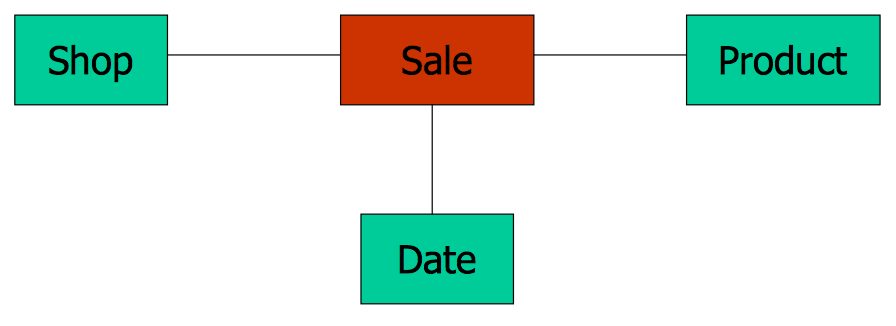
\includegraphics[width=\linewidth]{images/star.png}
  \caption{Star Model}
  \label{fig:star}
\end{figure}
An important analisys is related to the dimensions of the data warehouse, supposing: to store 2 years of data, for 300 shops for 3000 product sold every day in every shop, the fact table reach the dimensions of 660 milions of row (around 20GB of data).\\
The main operations over this kind of data is the computation with aggregated functions, with more complex operand (moving average, top ten, etc...) or applications of data mining techniques. This important evaluation are unusefull if the data is presentate bad.
\paragraph{Architecture} the system is build on several block:
\begin{itemize}
  \item Data Sources: External source, the DB.
  \item Data Warehouse: The big system.
  \item Data Marts: Smaller data warehouse related only to a single departement.
  \item OLAP servers: Multi dimensional data rappresentation.
  \item Metadata: Schemas information.
\end{itemize}
The data warehouse contains all the information on the company business and it requires a long time to be developed, the data mart are departimental information subset focused on a given subject, the implementation is faster than the warehouses, they requires a careful design. The data mart could be dependent (fed by the company warehouse) or independent (fe ddirectly by the sources). The most know solutions are:
\begin{itemize}
  \item \textbf{ROLAP}: (Relational OLAP)
  \begin{itemize}
    \item Extended relational DBMS (not sparse).
    \item SQL extension for aggrgate computation.
    \item Specialized access methods which implement efficient OLAP data access.
  \end{itemize}
  \item \textbf{MOLAP}: (Multidimensional OLAP)
  \begin{itemize}
    \item Data rappresented in multidimensional matrix (sparse data required compression).
  \end{itemize}
  \item \textbf{HOLAP}: (Hybrid OLAP) use MOLAP for fast and user stats and ROLAP for high detailed data.
\end{itemize}
There are 3 different solution for the system architecture, 1,2 and 3 level.\\
The first it better to be avoided, is not a good choice to have DBMS and DW on the same side. The other two are, the 2 level rappresented in figure \ref{fig:2lv}.
\begin{figure}[h!]
  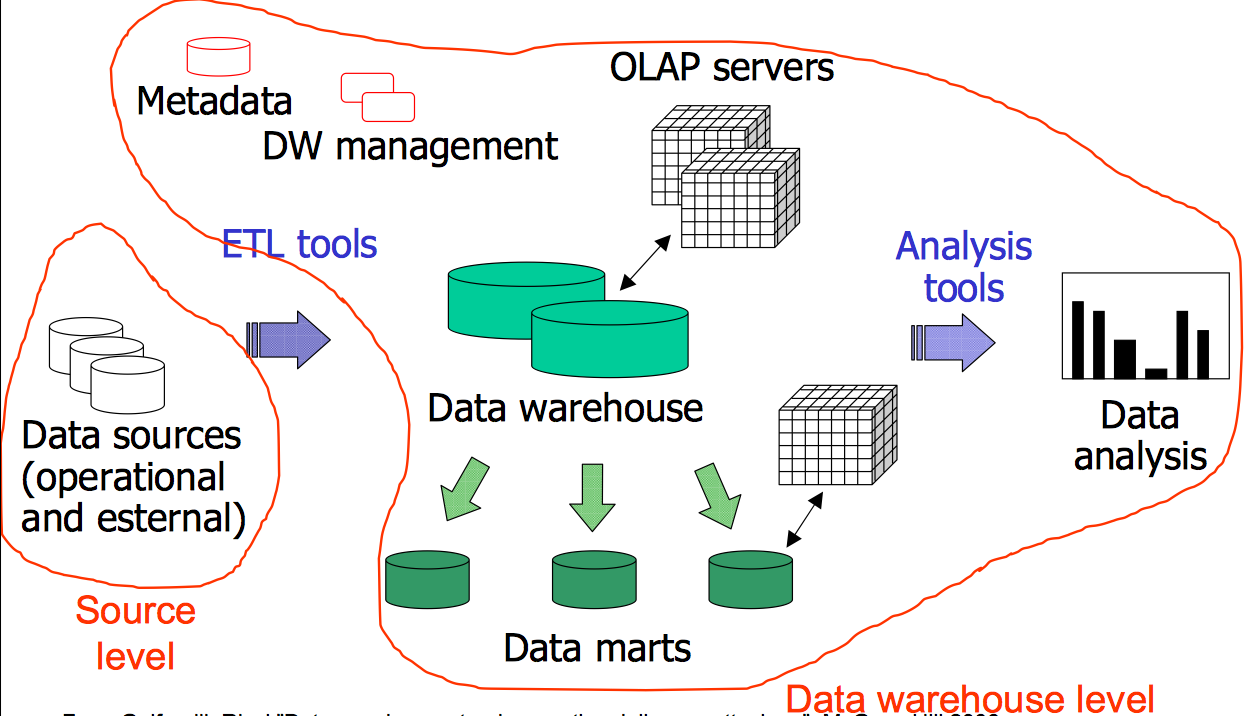
\includegraphics[width=\linewidth]{images/2lv.png}
  \caption{Two Level Architecture}
  \label{fig:2lv}
\end{figure}
These solution split the data and the DW, the only problem is data as soon as the data is added an "On the fly" data transformation is requires. Instead, in the three level solution (figure \ref{fig:3lv}), the problem is avoided introducing a staging area used for managing and cleaning operation.

\begin{figure}[h!]
  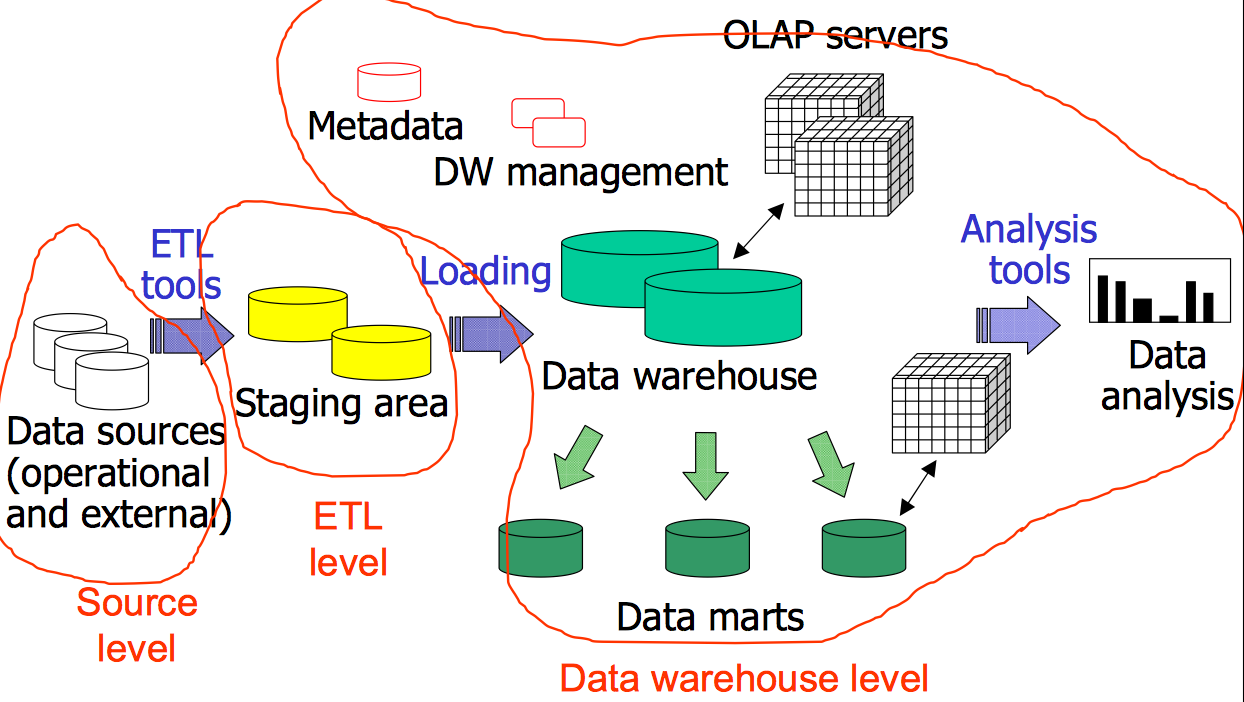
\includegraphics[width=\linewidth]{images/3lv.png}
  \caption{Three Level Architecture}
  \label{fig:3lv}
\end{figure}

\paragraph{ETL} Extraction, Transformation, Loading this process prepares data to be loaded into the data warehouse, is usually performed during the first load of the DW or during periodical DW refresh. The part are:
\begin{itemize}
  \item \textbf{Data Extraction}: Data acquisition from sources.
  \item \textbf{Data Cleaning}: Techniques for improving data quality (correctness and consistency).
  \item \textbf{Data Transformation}: Data conversion from operational format to DW format.
  \item \textbf{Data Loading}: Update propagation to the data warehouse.
\end{itemize}

\paragraph{Metadata} these are data about data. There are different types:
\begin{itemize}
  \item Data transformation and loading: Describe data sources and needed transformation operations.
  \item Data management: Describe the structure of the data in the DW, also for materialized view.
  \item Query management: Data on query structure and to monitor query execution (execution plan, memory and CPU usage).
\end{itemize}

\subsection{Design}
Using this type of structures involve some risks. Often the user think that data warehousing can solve the company's problems but is not like this, the behavior of this system is to provide that to solve in a better way the problem, not to solve problem. Also the source data could generate problems, incomplete or unreliable, also non itegrated or non optimized business processes. Good idea could be "politically correct" and developing a easy-to-use system.\\
\paragraph{Approach} there are two types of development:
\begin{itemize}
  \item \textbf{Top-Down}: Global and complete representation, complex and expensive.
  \item \textbf{Bottom-Up} incremental growth, separately focused on specific business areas.
\end{itemize}
in general the system follow a common flow, the Kimball lifecycle is a good rappresentation.\\
The data mart design:
\begin{itemize}
  \item Operational source schemas
  \item Reconciled schema: Not easy do design.
  \item User Requirements
  \item Fact schema: non standard rappresentation, usefull for developing.
  \item Feeding: Define script for saving data.
  \item Physical Design: Good system for improving performance.
\end{itemize}

\paragraph{Requirement Analysis} the first phase of designing is the analysis of the whole problem. We need to know:
\begin{itemize}
  \item Collects: The data needed in the data mart and the constraints related to previous information system.
  \item Sources: Business user and operational system administrator.
  \item Select: Is good to strat from the most important sector of the company and feeded by few reliable sources.
\end{itemize}
The application requirements, what we need to keep in the data mart, are different:
\begin{itemize}
  \item Description of relevant facts: Could be sales, phone call, investements, etc... With its usefull information (dimension). Granularity and time span.
  \item Workload: From already existent report generate new report. Other stuff produced in natural language.
\end{itemize}
There are also some structural requirements:
\begin{itemize}
  \item Feeding periodicity: Different from realtime or weekly reports.
  \item Available space
  \item System architecture: 1, 2 or 3 level.
  \item Deployment: Start up and training.
\end{itemize}

\paragraph{Conceptual Design} there isn't a standard model for this of kind of design, the dimensional fact model is proposed from Golfarelli e Rizzi in their book. This model define, for a given fact, dimensions, hierarchies and measures. The part are, figure \ref{fig:conce}:
\begin{itemize}
  \item \textbf{Fact}: It evolvs in time modelling a relevant events (ex. sales).
  \item \textbf{Dimension}: Describes the coordinate of the fact (ex. sales date, shop, etc...).
  \item \textbf{Measure}: Describes a numerical property of the fact (ex. number of sold unit).
\end{itemize}
\begin{figure}[h!]
  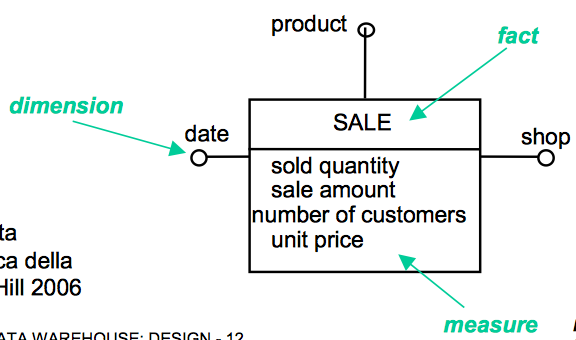
\includegraphics[width=\linewidth]{images/conce.png}
  \caption{Conceptual Design}
  \label{fig:conce}
\end{figure}
The hierarchy is the collection of all associated attributes of each dimensions. The attributes describe the dimension at different abstraction levels, this hierarchy represent a generalization relationship among subset of attributes in a dimension. Each edge represent a functional dependency 1:n. An example of hierarchy is: $Shop \rightarrow ShopCity \rightarrow Region \rightarrow Country$.\\
There some advanced features in these model:
\begin{itemize}
  \item Non-additivity: Not aggregatable over sum.
  \item Optional edge
  \item Convergence: Two different hierarchy converge at the sime point at the end of its.
  \item Optional dimension: Not always existent dimension.
  \item Descriptive attribute: Not aggregatable for computation, only descriptive.
\end{itemize}
there other stuff likes:
\begin{itemize}
  \item Multiple Edge: Relation n:n instead of 1:n.
  \item Shared Hierarchy: Different role from the same subset of data.
\end{itemize}

An interesting situation could be when the rappresentation of a fact without measure, is called factless fact schema. It can occur when you need to record the occurrence of an event, count the number of occurrence or representing events not occurred.

\paragraph{Aggregation} computes measures with a coarser (less fine) granularity than those in the original fact schema. The reduction is obtained climbing the hierarchy. The standard operator are SUM, MIN, MAX, AVG, COUNT.\\
The measure can be additive, not additive (by SUM), not aggregable. Measure can be of 3 type:
\begin{itemize}
  \item \textbf{Stream}: Evaluable at the end of a time period, aggragable by all operators (ex. sold quantity).
  \item \textbf{Level}: Evaluated at given time (snapshot), not additive along the time dimension (ex. Balance).
  \item \textbf{Unit}: Evaluated at a given time and expressed in relative terms, not additive (ex. Unit price product).
\end{itemize}
When is possible to compute aggregate from view of already aggregated value these operators are called \textbf{distributive}. Not all operators are distributive, AVG is \textbf{algebraic}, these types can compute higher level aggregations from more detailed data only when supplementary support measures are available. There is also another type called \textbf{Olistic} that can't compute aggregate from more detailed data.

\paragraph{Time Representation} the data modification over time is explicitly represented by the event (ex. time of buying, timestamp measurement). Also dimension could be change, the number of professors, the number of stores, etc... The only difference is related to the speed of change, this is named \textit{slowly changing dimension}.\\
The first (\textbf{TYPE I}) solution of this problem is to overwrite the data with the current value, this is used when the change is not important for the system like solving an error in a surname. This project the new situation over the past events. The second (\textbf{TYPE II}) solution is to directly correlate the events with the corresponding dimension value. This could be achived partitioning the data and creating a instance of the dimension. For example, \textit{Purchases performed by \underline{married} Mario Rossi} and \textit{Purchases performed by \underline{unmarried} Mario Rossi}.
The last solution (\textbf{TYPE III}) is similar to the type II because it create a new instance of the dimension, but it introduce a validity time stamp (start/end) for the dimension and a new attribute which allows to identify the root of the all dimension. The main utility of the last type is the projection to the future or to the past of and identity.\\

For example:\\
\textit{If we have a geo sub-division like nord-ovest and we compute the sels 2016 of this area, if we move one store to the area nord-center the computation of the sels of 2016 get a different results. Supposing to calculate the sels of the 2017, if we want to look at the results of the old nord-ovest configuration, but with the new data, the only solution is to use the TYPE III representation. }\\

The third solution must be used only if the system really need this because could be really coplicated to be mantained.

\paragraph{Other} the workload must be defined during the design phase, this can depends on user number, complexity and dimension. Probably a phase of tuning will be necessary for improving the system work.\\
The estimation of data volume is necessary due to a correct development of the system. Everything must be considered, from indicies, to materialized view, to time span, attribute length, etc.. This because this type of structure everything could become really big. Difficulties on volume estimation come from sparsity, because when we reducing granularity, with a high sparse cube, the reduction factor could be greater that expected.

\paragraph{Logical Design} this phase start from the relational model (ROLAP):
\begin{itemize}
  \item Conceptual fact schema
  \item Workload
  \item Data Volume
  \item System Constraints
\end{itemize}
Is a litle bit different from the traditional logical design because the data redundancy (lose of normalization) is acceptable due to a performance improve. Is a good idea to ad redundancy only in the dimension table and not in the fact table, because the number of records is really really bigger in the second one.
The star schema (figure \ref{fig:bigstar}) is composed by:
\begin{itemize}
  \item Dimensions:
  \begin{itemize}
    \item One table for each dimension
    \item Surrogate primary key (counter)
    \item It contains all dimension attributes
    \item Not explicit hierachies respect ROLAP schema
    \item Totaly denormalized representation
  \end{itemize}
  \item Facts
  \begin{itemize}
    \item One fact table for each fact schema
    \item Primary key composed by foreign keys of all dimensions
    \item Measures are attributes of the fact table
  \end{itemize}
\end{itemize}

\begin{figure}[h!]
  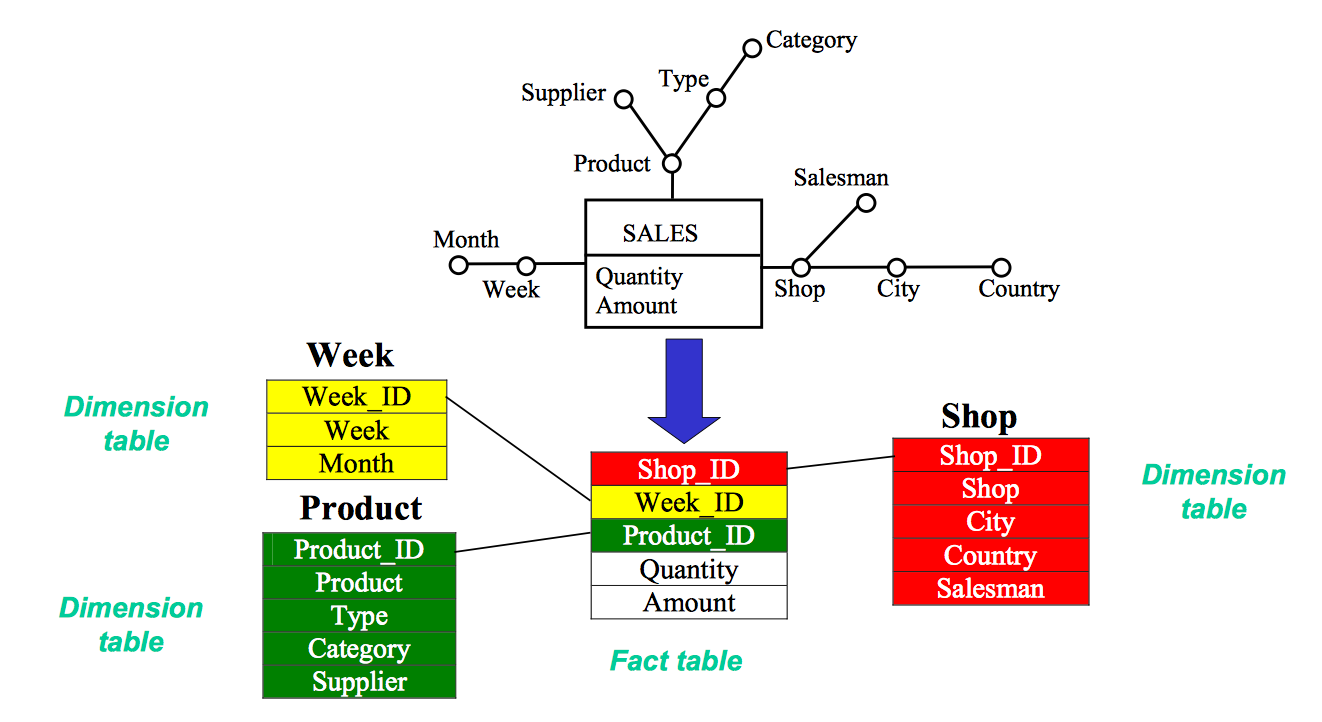
\includegraphics[width=\linewidth]{images/bigstar.png}
  \caption{Star Schema}
  \label{fig:bigstar}
\end{figure}

Directly from the star schema we can derive the \textbf{Snowflake} schema that introduce a bit of normalization to reduce the size of the dimension table. This representation is created spliting in two or more table one dimension table, an example in figure derived directly from the previous star schema.

\begin{figure}[h!]
  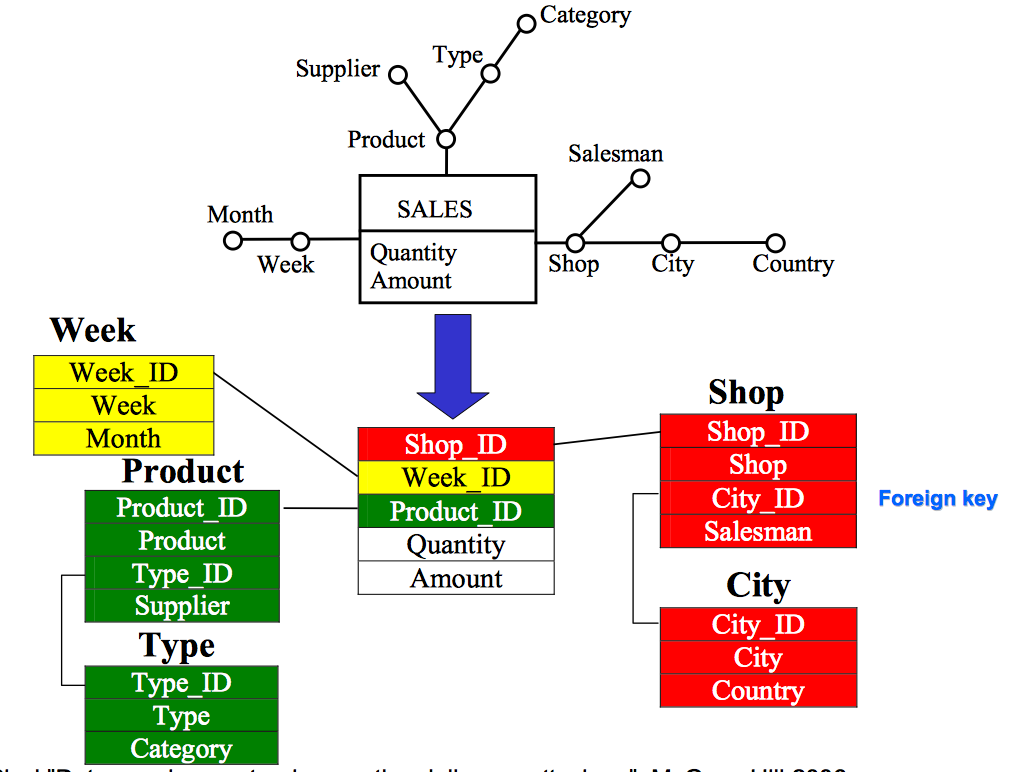
\includegraphics[width=\linewidth]{images/snowflake.png}
  \caption{Snowflake Schema}
  \label{fig:snowflake}
\end{figure}

The main advantage are related to some space optimization, the disadvantage is that this solution need one or more further join. Normally the star schema is preferred. The only cases could be when one part of one dimension is shared above more dimension.

\textbf{Multiple edges} needs an appropriate implementation, there are two solution:
\begin{itemize}
  \item \textbf{Bridge Table}: similar to classic relational schema add a table between the two tables linked by the edge to "merge" the cases. This solution allow to adds usefull attributes, like weight for computing specific calculations (ex. author income in a not equaly divison book).
  \item \textbf{Push Down}: Add 2 keys to the fact table. The weight in this case is wired in the fact table. The PD add problem related to increase of redundancy, the only advantages is a minor number of join required.  NOT GOOD SOLUTION.
\end{itemize}

In some cases could be necessary to create a dimension with only one attribute for a dimension, this is named \textbf{degenerate dimension}. There are two options to overcome the problem:
\begin{itemize}
  \item Attribute directly integrate into the fact table (only attribute with very small size).
  \item Junk dimension: A single dimension containing several degenerate dimensions with no functional dependencies among them.
\end{itemize}

\paragraph{Materialized Views} respect the view, the materialized ones, are table from all aspects are they aren't computed at the time the view is requested. The materialized implements an already aggregated result of a previous interrogation of the fact table. They are used for improve the performance during the computation of query less detailed. An example in figure \ref{fig:matview}.
\begin{figure}[h!]
  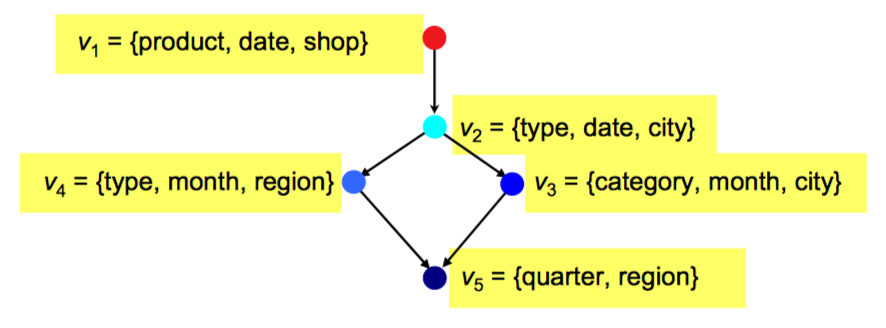
\includegraphics[width=\linewidth]{images/matview.png}
  \caption{Example of materialized view}
  \label{fig:matview}
\end{figure}
The views are SQL statement,  generated starting from base tables or view with higher granularity. Considering that this views can takes up a lot of space is better to used their only when the are really usefull. A good advice is to develop views that are used from a lot of interrogation. Of course, generating a view that include a lot of aggreation attributes can be to big to be mantained, also the space occupied could be to much. In general the idea is to minimize this values:
\begin{itemize}
  \item Disk space
  \item Update window
  \item Query cost
\end{itemize}

During the physical development of a data warehouse is important to manage the workload. The queries are computed with a lot of aggregation level and they will probably access to an huge part of each table involved. One of the main advantage of this system is the they are read-only and they don't require to be modififed. A periodical scheduled refresh is needed to keep the data valid, also indicies and other stuff.\\
Respect the OLTP this type of system use different index types like bitmap, join, bitmapped join index, etc...\\
An important phase of the development is the tuning where, looking at the real utilization behaviour the system if fitted to improve performance during real-life application. This phase is also used in case of structural changes. In more complex environment the parallelism become important, it can really increase the performance.\\
The index selection is performed on:
\begin{itemize}
  \item Attributes frequently involved in selection predicates.
  \item High cardinality domain, with B-tree index.
  \item Low cardinality domain, with bitmap index.
\end{itemize}
Indexing only foreing keys in the fact table is rarely appropriate because the index could become big like the table reducing the real advantages of this stuff.

\paragraph{ETL} the Extraction, Transformation and Loading phases are fundamental to prepare data to be loaded into the warehouse. Is performed at the first DW load and during periodical refresh, it's involve:
\begin{itemize}
  \item Data extraction from OLTP or external sources.
  \item Data Cleaning.
  \item Data transformation.
  \item Data loading.
\end{itemize}
The process is eased by using the staging area. In general this phase is different if the system is during the first load or if is a periodical update/\\
The \textbf{extraction} acquire the data from the sources. If is the first time performa a \textit{static} extraction grabbing snapshot of operational data. If is an update, it will use an \textit{incremental} solution to extracting data since the last update only. In case of multiple sources is important to choose the best one. Of course is important to analyze how the data is collected:
\begin{itemize}
  \item \textbf{Historical}: All modification, with a datastamp, are stored for a given time in the OLTP system (bank transaction, exam, etc...).
  \item \textbf{Partly Historical}: Not all the modification are stored, only a limited number of state.
  \item \textbf{Trasient}: Only the current data state is keeps on the OLTP.
\end{itemize}
Of course the real challenge is over trasient data.\\
The incremental extraction comparing 2 snapshot of the system it's a mess. One solution to this problem is to be \textbf{assisted by the application}, this means force the OLTP system to keep track of modification, on the selected table, in dedicated table. This means doubling the application load because every insert or update must be performed 2 times. This is the last solution, just used only on legacy system, because require a modification directly in the applications that perform the modification.\\
The best solution is using the \textbf{log}, this is written in any case for recovery pourpose, this means that using the log not require unnecessary data operations. Both operations are performed at the same time that the main transaction is done, are immediate.\\
Another possibile solution is using the \textbf{triggers}, there is the duplication like the application support, but this solution not require editing the single application, but editing only the DBMS.\\
The last solution is using the \textbf{timestamp}. The system need a new attribute for the \textit{last modification time}. During the data extraction, first the system will find the first \textit{"not yet added"} record, and then will start to scan the table from this point. This is the only deferred extraction and it means possible lose of intermediate state if the data is transient. A fast comparison over the various techniques in figure \ref{fig:extraction}.

\begin{figure}[h!]
  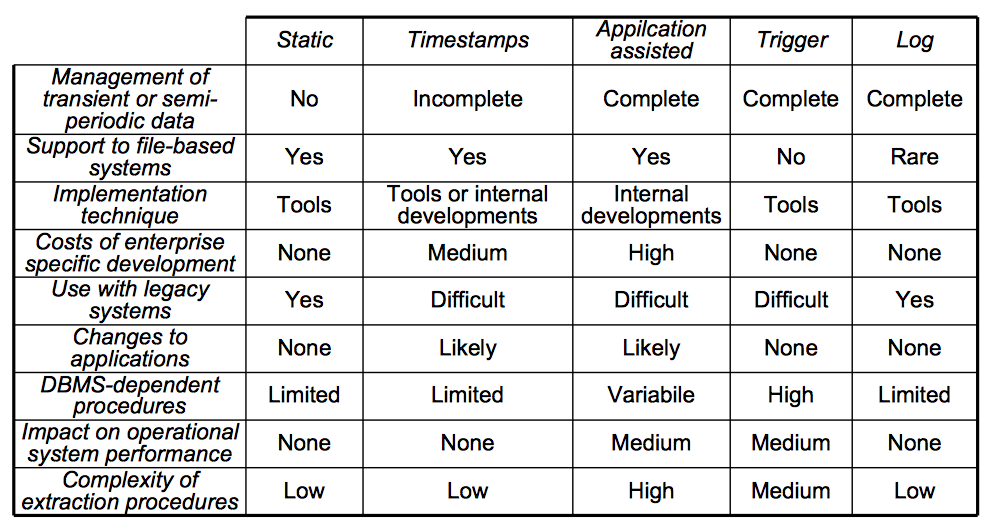
\includegraphics[width=\linewidth]{images/extraction.png}
  \caption{Comparison of extraction techniques}
  \label{fig:extraction}
\end{figure}

Another important phase of the ETL is the \textbf{cleaning}. That phase have the task to clean all the data problem related to entry errors, different field formats and for evolving business pratices. This means remove duplicate, fill missing data, correct wrong use of field, remove impossibile or wrong data and all the other inconsistency correlated. That problem can be solved using \textbf{data dictionary} used for entry or format errors. This of course can be performed only over data domains with limited cardinality. Another solution could be the \textbf{approximate fusion}, these techniques tries to find duplicates or similar, with a defined criterion,  and perform operation to fix it when is possibile, otherwise the data must be purge again manually.\\

The \textbf{trasformation} required data conversion from the operational to the warehouse format. The phase is divide in two part:
\begin{itemize}
  \item From operational to the reconciled data in the staging area.
  \begin{itemize}
    \item Conversion
    \item Matching
    \item Data selection
  \end{itemize}
  \item From reconcilied to the data warehouse.
  \begin{itemize}
    \item Surrogate keys generation
    \item Aggregation computation (view, fact table, indices, etc...)
  \end{itemize}
\end{itemize}
the dimesion table loading is represented in figure \ref{fig:dimload} and the fact table loading in figure \ref{fig:factload}.

\begin{figure}[h!]
  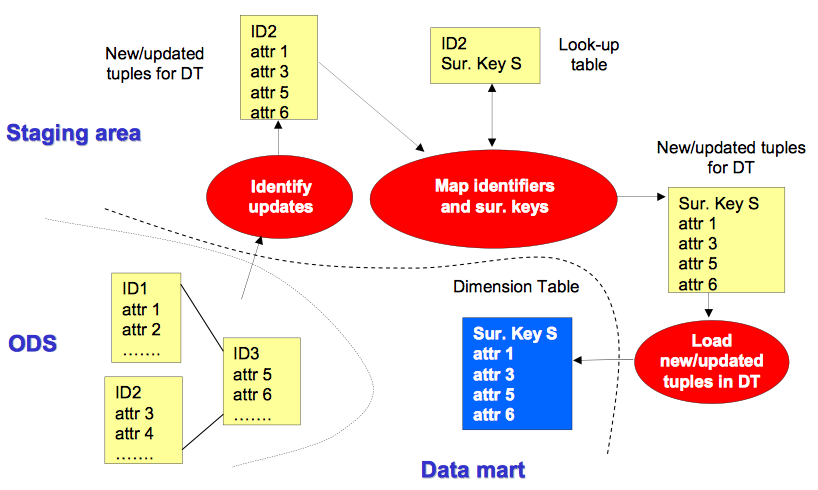
\includegraphics[width=\linewidth]{images/dimload.png}
  \caption{Dimension table loading}
  \label{fig:dimload}
\end{figure}
\begin{figure}[h!]
  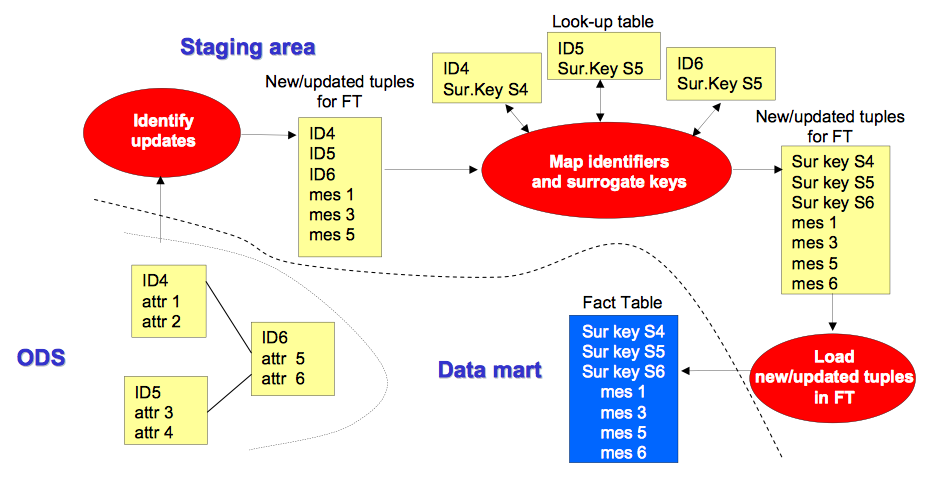
\includegraphics[width=\linewidth]{images/factload.png}
  \caption{Fact table loading}
  \label{fig:factload}
\end{figure}

\subsection{Data Analisys} % 3-DWquery-EN-2x
The analisys over data warehouse is slightly different from the normal query over relational DB. The OLAP analisys require to compute complex aggregate function for aggregation, for comparisons or data mining. The normal SQL isn't enough confortable to be used for this kind of computation. The datawarehouse could be query by various tools:
\begin{itemize}
  \item Controlled Query Environments
  \item Query and Report generation tools
  \item Data mining
\end{itemize}
In the \textbf{Controlled query environment} have always a predefined structure with complex query, ad hoc analisys procedures and predefined reports. This environment requires ad hoc code development, stored procedures, predefined joins, aggregation and so on. Also some useful and flexible package for a better and easy-to-use report management are available. The system could be also fitted to use KPI of a specific economic area, like economical or finacial indicators.\\
When the CQE is not enough for the user a solution can be to develop an \textbf{Ad hoc query environment}. With this solution the user can define OLAP queries with a point and click techniques that generates SQL code, this means that the user must know a little bit the data structure of the warehouse. THe advantage is that, like the CQE, the user can exploits complex query with spreadsheet reports techniques.

\paragraph{OLAP Analisys} this adds some useful operations to perform more complex query.\\
The rollup is a technique used for decreasing the data detail, this could be obtained by climbing up the hierarchy, from \textit{group by store, month} to \textit{group by city, month}, or dropping a whole dimension, from \textit{group by product, city} to \textit{group by product}. The drill down is the opposite of the rollup, it increase the data detail add a whole dimension or wakling dow the hierarchy. This operation could generate some problem related to spare matrix and data explosion, is problem can be solved using the slice and dice technique. This last operations selects a data subset by means of selection. The \textit{slice} means selecting a slice not changing the granularity but adding only a equality predicate, the \textit{dice} try to reduce the information of the slice over some reduced set. The result of this operation in figure \ref{fig:sd}, over the data in figure \ref{fig:sd_start}.
\begin{figure}[h!]
  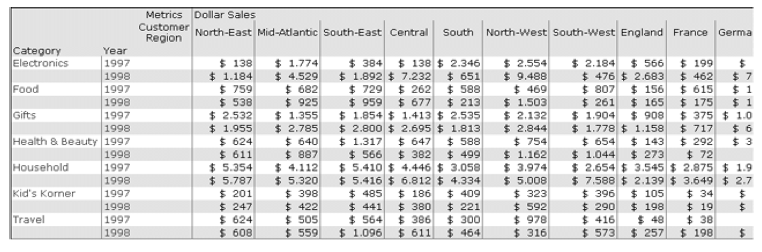
\includegraphics[width=\linewidth]{images/sd_start.png}
  \caption{Starting table}
  \label{fig:sd_start}
\end{figure}
\begin{figure}[h!]
  \centering
  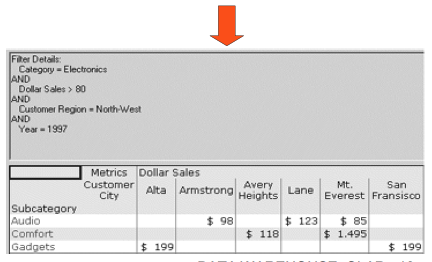
\includegraphics[width=0.8\linewidth]{images/sd.png}
  \caption{Table sliced and diced}
  \label{fig:sd}
\end{figure}
The last operation is the pivot, this solution reorganize the multidimensional structure, swapping the axises, without varying the detail level, this could be confortable to increase the readability of the same information.

\paragraph{Extension of SQL language} this extension was introduced to support, in a better way, the new computation request of the data warehouse world. The were also standardized from the ANSI.\\
The computation window is a new clause introducted by the extended SQL. Is charaterized by:
\begin{itemize}
  \item \textbf{Partitioning}: Rows are grouped, like \textit{group by}, but without collapsing them.
  \item \textbf{Reordering}: Rows are ordered inside its group created by the partitioning.
  \item \textbf{Aggregation Windows}: It defines where perform the aggregation.
\end{itemize}
Example:\\
\textit{Show, for each city and month: (1) Sales amount and (2) Average on the current month and the two previous months, separately for each city.} The query will be:
\begin{figure}[hp!]
  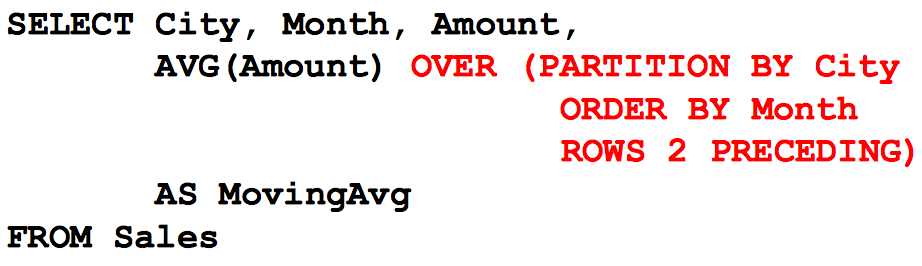
\includegraphics[width=\linewidth]{images/avg.png}
\end{figure}\\
Some consideration over this function: The sort order is required altought the computation of the window become inconsisten. When the window is not complete, like end of the month, the computation takes place on the available rows. Is possible to use several window at the same time. The aggregation window may be defined in two ways:
\begin{itemize}
  \item Physical Level: It builds the group by counting rows (\textit{current and 2 preceding \textbf{rows}}).
  \item Logical Level: It builds the group by defining and interval on the sort key (\textit{current and 2 preceding \textbf{months}}).
\end{itemize}
both of this solution can implement a variable window using PRECEDING, BETWEEN and FOLLOWING. Is also posbbile to defined an UNBOUNDED window that change its size during that computation using only one fixed bound, useful for cumulative total. The difference is that the physical one not look at missing rows and is possibile to order by more than one keys. Altought the logical can perform ordering only over numerical or data type where a distance can be defined and only by one key at the time. Another important characteristics is the possibility to compare detailed and total data without problem.\\
There is also a Ranking function that computes the rank of a value inside a partition, it could be of 2 types, \textbf{rank()} that computes the rank by leaving an empty slot after a tie, and \textbf{denserank()} that rank by leaving an empty slot after a tie. Of course this function requires an ordering altought would be meaningless, the partition is not necessary because it can compute also over the whole table. Is important to notice that the order by of the over is not the visualizing order, but is only the order for the ranking, if a ordered visualization is needed an external group by is compulsory.\\
The main important extension is related to the \textit{group by} that allows to compute multiple aggretation without performing separte query, this increase the efficency of the whole system.\\
Using the rollup function over that computes multiple aggregates one at a time. The order in the expression is fundamental, it will compute the aggregate starting with all attribute and removing it one by one from right to left. The visualization of this computation have NULL value to represents the superaggregates, an example in figure \ref{fig:rollup}.
\begin{figure}[h!]
  \centering
  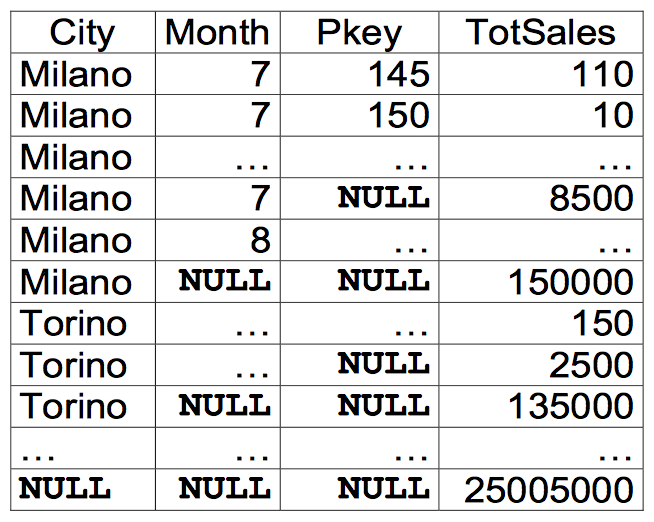
\includegraphics[width=0.8\linewidth]{images/rollup.png}
  \caption{Rollup with 3 values}
  \label{fig:rollup}
\end{figure}
In this figure the first row with NULL present the total for the 7th month for Milano, the second one, with 2 NULL, is the total of all months for Milano, the last one, with 3 NULL, is the total for all months, for all cities.\\
The \textbf{cube} function is used for computing all aggregates of all possible combination, in this case the order of the parameters is not important. This function is like performing more rollup at the time, is also well implemented respect software computation.

%--------------------------------------------------------------------------------------------------------
%--------------------------------------------------------------------------------------------------------
%--------------------------------------------------------------------------------------------------------
\clearpage
\section{Data Mining}
\subsection{Introduction} \label{subsec:datamin_intro}
During this year the companies the number of database and its size it increased a lot. All DB are potential source of useful information. Is know the our capacities of collecting data is really more the out capacity of analyzing it.\\
The \textit{data mining} is:\\
\noindent\fbox{
  \parbox{\textwidth}{\textit{Non trivial extraction of \textbf{implicit}, \textbf{previously unknow} and \textbf{potentially useful} information from available data}.}
}\bigskip

Of course, our pourpose, is to extract in an automatic way the information to represent it with abstracted models denotated pattern.\\
One example of this technique application is the profiling from e-commerce, search engines, social, georeference data, etc... These profling will be used for mirated advertisement, market basket analysis, brand reputation, sentiment analysis, etc...\\
Another important application of these techniques could be the biological data analysis for mapping DNA, demographic data, illnesses diffusion, etc...\\
The flow of the data analysis is named KDD, \textit{Knowledge Discovert from Data}, a rappresentation in figure \ref{fig:kdd}.
\begin{figure}[h!]
  \centering
  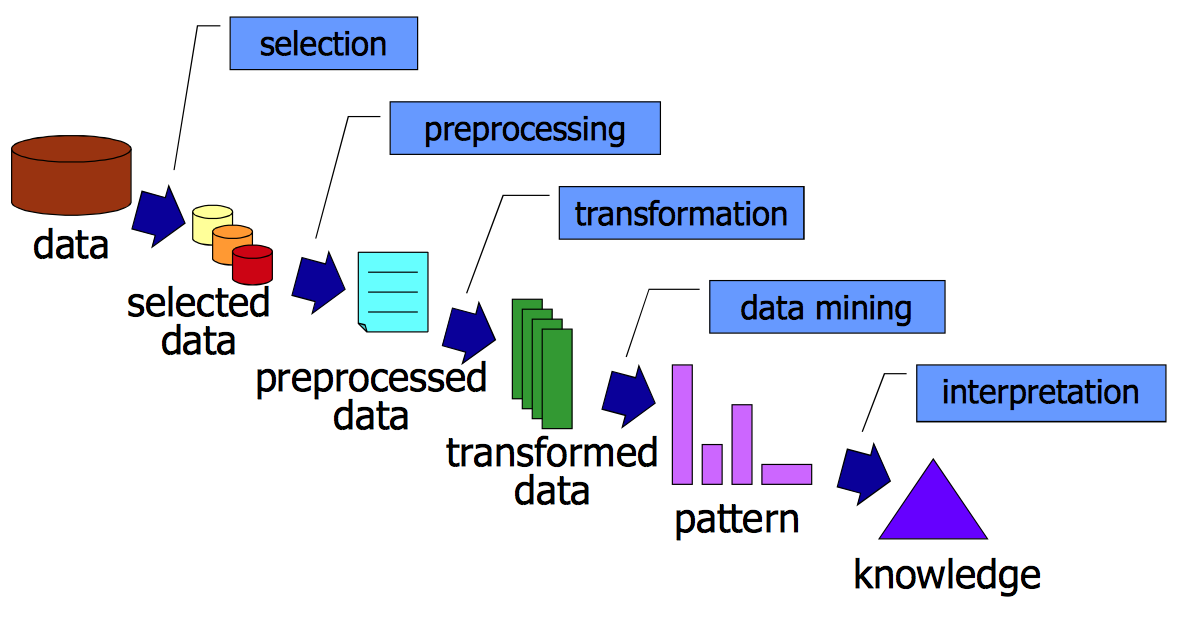
\includegraphics[width=0.9\linewidth]{images/kdd.png}
  \caption{Knowledge Discovert from Data}
  \label{fig:kdd}
\end{figure}
The first step is the data selection. Starting from a big source, like a data warehouse, only a part of this repository will be used. The preprocessing phase is similar to the ETL phase, it perform data cleaning and data integration to generate data fitted for the mining. A good quality is needed, no good quality, no good quality pattern.\\
The data mining origins start from the statics, now are also used for machine learning, pattern recognition and database systems.\\
The are two types of analysis techniques, the \textbf{Descriptive method} that extract interpretable model describing data starting from pattern. Are useful for client segmentation for example. Another technique is the \textbf{Predictive methods} exploits some know variables to predict unknow or future values of other variables. An example could be the spam filter. This technique can't predict anomal events, not linke to the previuos history.\\
Some of the most important predictive methods are the \textbf{classification} this try to predict a class label by defining an interpretable model of a given phenomenon.\\
How this it works?\\
After a traning phase where the system understand from a traning set, where all data is labelled, the system define a model to parse unclassified data for correctly classifing it. Some examples are:
\begin{itemize}
  \item Decision tree
  \item Bayesian classification
  \item Neural networks
  \item SVM
\end{itemize}
The selection of the methods to be used depends on accuracy, interpretablity, scalability, noise and outlier management. A more accurate process probably generate uninterpretables models and so on. There isn't a final technique, every problem need a fitted solution.\\
Another important predictive methods is the \textbf{clustering} that try to detect groups of similar data objects, computing distance, and identifying exceptions and outliers. The k-means is an example, like SOM or density-based. In these techniques the requirements are similar to the previous one, with more importance over the scalability and the noise managements. These results are really hard to be interpreted and this is why are often passed to a classification phase.\\
The \textbf{association rules} are newer and its behaviour is to extract frequent correlations or pattern from a transactional database. One of the most know result of this technique was the \textit{Diapers $\rightarrow$ Beer} correlation. Using these methods allow solution for cross-selling, market basket analysis and shop layout design.\\
There are important, still open, issues related to:
\begin{itemize}
  \item Scalibility to HUGE data volumes.
  \item Data dimensionality.
  \item Complex data structues, heterogeneous data formats.
  \item Data quality.
  \item Privacy preservation.
  \item Streaming data.
\end{itemize}

\subsection{Data preprocessing}
There are several data set types:
\begin{itemize}
  \item Record
  \begin{itemize}
    \item Tables
    \item Document
    \item Transaction
  \end{itemize}
  \item Graph
  \begin{itemize}
    \item WWW: Link from page to page
    \item Molecular Structures
  \end{itemize}
  \item Ordered
  \begin{itemize}
    \item Spatial data
    \item Temporal
    \item Sequential
    \item Genetic Sequence
  \end{itemize}
\end{itemize}

The tabular data is a collection of record characterized by a fixed set of attributes. Presenting documents data is performed transforming it in a vector of terms. In this cases an important phase is the filtering of stock word (grammar article, word to singular, verbs to infinite, etc...).\\
There are different types of attribute:
\begin{itemize}
  \item \textbf{Nominal}: ID Numbers, eye color, zip codes, etc... (D)
  \item \textbf{Ordinal}: Rankings, grades, height, etc... (DO)
  \item \textbf{Interval}: Calendar dates, temperatures, etc... (DOA)
  \item \textbf{Ratio}: temperature Kelvin, lenth, time, counts, etc... (DOAM)
\end{itemize}
the types depends on which of the following prepertis it possesses:
\begin{itemize}
  \item \textbf{Distinctness}: =, $\neq$
  \item \textbf{Order}: $<$, $>$
  \item \textbf{Addition}: +, -
  \item \textbf{Multiplication}: *, /
\end{itemize}
another characterization is \textbf{discrete} or \textbf{continous} types.\\
The data quality is really important. Noise, outliers or missing values can generate a problems and must be managed for a correct data usage. There are a lot of reasons for missing values, from information not collected to attributes not applicable to all cases. In both case they must be handled by:
\begin{itemize}
  \item Eliminate data objects
  \item Estimate missing values
  \item Ignore the missing value during analysis
  \item Replace with all possible values.
\end{itemize}

The preprocessing phase is divided in more step. The \textbf{aggregation} cobine two or more attributes into a single attribute. The purpose is to perform data reduction, change of scale and getting more "stable" data. The \textbf{data reduction} generates a reduced representation of the sataset. This rappresentation is smaller in volume, but it can provide similar analytical results. The techniques used to perform this tasks are:
\textbf{Sampling} that is employed for data selection. Samples are easier to be used, because they are really little respect the entire sets and they become less expensive from the point of expenses and time consuming. Of course the idea is to preserve the quality of the entire set. There are several types of sampling:
\begin{itemize}
  \item Simple Random Sampling: Equal probability.
  \item Without replacement: Each selected item is removed from the population (difference on probability).
  \item With replacement: Not removed from population, the item could be a duplicate.
  \item Stratified: Preserve the distribution of the starting schemes, performing random selection inside the single partition.
\end{itemize}

The \textbf{curse of Dimensionality} says that \textit{when dimensionality increases, data becomes increasingly sparse in the space that it occupies}. On solution is to perform \textbf{dimensionality reduction}, it tries to reduce the amount of time and memory required by the algorithms, allow data to be more easilty visualized and may help to eliminate irrelevant features or reduce noise. The principal techniques used are:
\begin{itemize}
  \item Principle Component Analysis: Merge data point on a vector, missing physical idea.
  \item Singulat Value Decomposition.
  \item Others: Supervised and non-linear methods.
\end{itemize}
Another way to reduce the dimensionality of data is to reduce the redundant features, for example: \textit{purchase price of a product and the amount of sales tax paid}. Also removing irrelevant features is useful. How can i do this? There are several techniques:
\begin{itemize}
  \item Brute-Force: Try all possible feature as input.
  \item Embedded: Feature selection occurs naturally as part of the algorithm.
  \item Filter: Selection before the run.
  \item Wrapper: Use the algo like a blackbox to find best subset of attributes.
\end{itemize}
Is also possible to create a new feature that can capture the important information in a data set much more efficiently than the original attributes. Thi can be achived with: Feature extraction, mapping to new space and feature construction.\\
The last part of data reduction is the \textbf{discretization} that split the domain of a continuous attribute in a set of intervals, reducing the cardinality of the attribute domain. Solutions:
\begin{itemize}
  \item N intervals with the same width ($W=(V_max - V_min)/N$): Badly affect by outliers and sparse data. Incremental.
  \item N intervals with (approximately) the same cardinality: Fits better outliers and spare, but not incremental.
  \item Clustering: Fit well sparse data and outliers.
\end{itemize}
an example in figure \ref{fig:discretization}.
\begin{figure}[h!]
  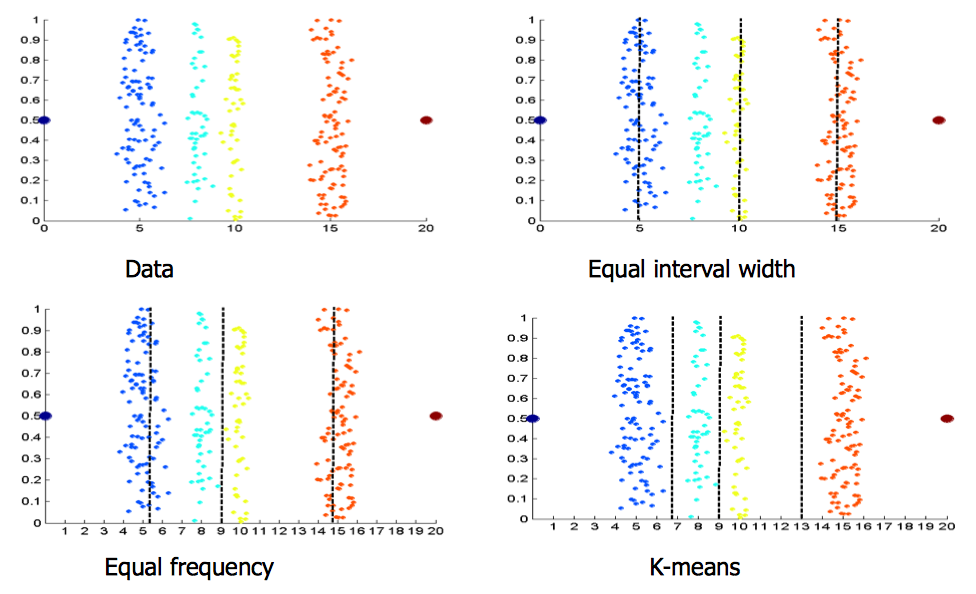
\includegraphics[width=\linewidth]{images/discretization.png}
  \caption{Discretization}
  \label{fig:discretization}
\end{figure}

In some cases an \textbf{attribute transformation} could be useful. Is a function that maps the entire set of values of a given attribute to a new set of replacement values such that each old value can be identifies with one of the new values. This normalization can be achieved with solution like: min-max normalization (rescaling), z-score and deciaml scaling.\\
A lot of operations are performed computing distances:
\begin{itemize}
  \item \textbf{Similarity}: Numerical measure of how alike two data objects are, high value implies similar object, often falls in [0,1] range.
  \item \textbf{Dissimilarity}: Numerical measure of how different two data objects are, lower means different objects.
  \item \textbf{Proximity} refers to a similarity or dissimilarity.
\end{itemize}
In case of a simple attribute the solutions are reported in figure \ref{fig:simdis}.
\begin{figure}[H]
  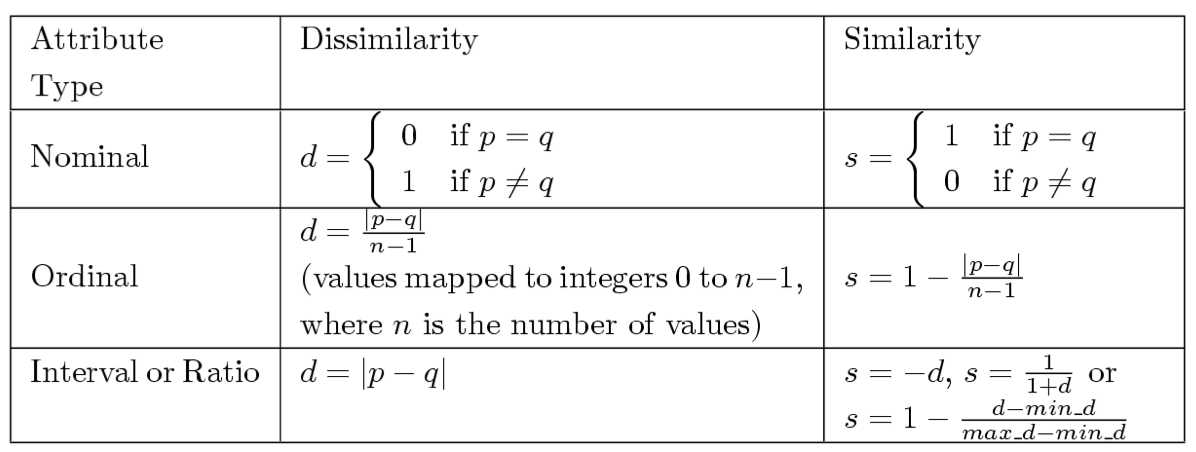
\includegraphics[width=\linewidth]{images/simdis.png}
  \caption{Similarity and Dissimilarity for simple attributes}
  \label{fig:simdis}
\end{figure}
When the similarty or dissimilarty must be computed over different attributes a more complex instruments is necessary, some examples are:
\begin{itemize}
  \item \textbf{Euclidean Distance}: $dist=\sqrt{\sum_{k=1}^{n}(p_k - q_k)^2}$ It requires standardization if scales differ.
  \item \textbf{Minkowski Distance}: $dist=(\sum_{k=1}^{n}|p_k - q_k|^r)^\frac{1}{r}$ this is the general case, the r=2 is the euclidean, r=$\inf$ is the supremum.
\end{itemize}

Is some cases could be also useful computing distances between binary vectors, one solution is using the simple matching that is: SMC = Number of Matches / Number of attributes $(M_11 + M_00) / (M_01 + M_10 + M_11 + M_00)$. The Jaccard coefficents instead calculate similarities with: J = number of 11 matches / number of not-both-zero attributes values $(M_11) / (M_01 + M_10 + M_11)$.\\
The final computation distance over 2 point with more attributes can be evaluated with the following formula:
\begin{equation}
  \begin{gathered}
    similarity(p,q) = \frac{\sum_{k=1}^{n} \omega_k \delta_k s_k}{\sum_{k=1}^{n} \delta_k}
  \end{gathered}
\end{equation}

\subsection{Association Rules}
The objective of the association rules is to extract frequent correlation or patterns from a transactional database. An example could be:
Diapers $/Rightarrow$ Beer that it means that, for example, 30\% of transaction containing diapers also contains beer. \textbf{It is not a cause-effect correlation!}.\\
A collection of a transaction is:
\begin{itemize}
  \item Set of items.
  \item Without order correlations between them.
\end{itemize}
The association rule extraction is an exploratory technique that can be applied to any data type. It can also be applied over textual data document, etc...\\

\paragraph{Definitions} An association rule is compesed by multiple parts:
\begin{itemize}
  \item \textbf{Itemset}: Set including one or more items.
  \item \textbf{k-itemset}: Itemset that contains k items.
  \item \textbf{Support count} (\#): Frequency of occurrence of an itemset.
  \item \textbf{Support}: Fraction of transaction that contains an itemset.
  \item \textbf{Frequent Itemset}: Itemset whose support is greater than or equal to a \textit{minsup} threshold.
\end{itemize}
We need also to define some rule quality metrics. Given the association rule A $\Rightarrow$ B (A, B are itemsets) the:
\begin{itemize}
  \item \textbf{Support}: Fraction of transaction containing both A and B: $(\#\{A,B\}/|T|)$
  \begin{itemize}
    \item $|T|$ is the cardinality of the transactional DB.
    \item A priori probability of itemset AB.
    \item Rule frequency in the DB.
  \end{itemize}
  \item \textbf{Confidence}: Frequency of B in transaction containing A: $(sup(A,B)/sup(A))$ [Conditional probability]
\end{itemize}
An example with data from table below:
\begin{center}
  \begin{tabular}{ |c|c| }
    \hline
    \textbf{TID} & \textbf{Items}\\
    \hline
    \hline
    1 & Bread, Coke, Milk\\
    \hline
    2 & Beer, Bread\\
    \hline
    3 & Beer, Coke, Diapers, Milk\\
    \hline
    4 & Beer, Bread, Diapers, Milk\\
    \hline
    5 & Coke, Diapers, Milk\\
    \hline
  \end{tabular}
\end{center}
From the itemset \{Milk, Diapers\} the following rules may be derived:
\begin{itemize}
  \item Rule: Milk $\Rightarrow$ Diapers
  \begin{itemize}
    \item Support: $\#\{Milk,Diapers\}/\#trans$ = 3/5 = 60\%
    \item Confidence: $\#\{Milk,Diapers\}/\#\{Milk\}$ = 3/4 = 75\%
  \end{itemize}
  \item Rule: Diapers $\Rightarrow$ Milk
  \begin{itemize}
    \item Support: 60\%
    \item Confidence: $\#\{Milk,Diapers\}/\#\{Diapers\}$ = 3/3 = 100\%
  \end{itemize}
\end{itemize}
Given a set ot transaction T, association rule mining is the extraction of the rules satisfying the constraints of the minimum support and confidence. That rules is not easy to be obtained.\\
During the execution of these extraction we like to have a \textbf{complete} (\textbf{all} rules satisfying both constraints) and \textbf{correct} (\textbf{only} the rules satisfying both constraints). This is true for the association rules, but not for all techniques that we will study during this course.\\
\paragraph{Extraction} The first easy solution is the \textbf{brute-force} approch, it:
\begin{itemize}
  \item Enumerate all possible permutations.
  \item Compute support and confidence for each rule.
  \item Prune all the rules that do not satisfy the threshold.
\end{itemize}
Of course this method is computationally unfeasible. The fisrt variation from the brutal method is the following. Given an itemset, the extraction process may be split:
\begin{enumerate}
  \item Generate frequent (passing the threshold) itemsets.
  \item Generate rules from each frequent itemset.
\end{enumerate}
The two step above have a lot of problem anyway, the first one can be performed with different techniques like Apriori, FP-growth, etc.. Best it still remain computionally expensive. The second one is more standard and it can be improved too much and is the generation of all possible binary partitioning of each frequent itemset. The BF approch have a huge complexity \textasciitilde $ O(|T| 2^d w)$ where d is the number of items and w the transaction length.\\
How to improving the efficiency?
\begin{itemize}
  \item Reduce the number of candidates.
  \item Reduce the number of transaction (e.g. Remove all the transaction with less then x items searching for y items).
  \item Reduce the number of comparisons.
\end{itemize}

\paragraph{Apriori Principle} [Agr94] is the first studied algorithm, it say that: "\textit{If an itemset is frequent, then all of its subsets must also be frequent}".\\
Of course the support of an itemset can never exceed the support of any of its subsets. This is guarantee by the antimonote property of the support measure: $if A \subseteq B \rightarrow sup(A) \geq sub(B)$. This allow a candidates reductions.\\
It's a level-based approch, at each iteration extracts itemsets of a given length k. For each level, two main steps are executed:
\begin{enumerate}
  \item Candidate Generation:
  \begin{itemize}
    \item Join Step: Generate candidates of length k+1 by joining frequent itemsets of length k.
    \item Prune Step: Apply Apriori principle: Prune length k+1 candidate itemsets that contain at least one k- itemset that is not frequent.
  \end{itemize}
  \item Frequent iteset generation:
  \begin{itemize}
    \item Scan DB to count support for k+1 candidates.
    \item Prune candidates below minsup.
  \end{itemize}
\end{enumerate}
The generation of candidates start ffrom $L_k$, that is the set of candidate of length k in a lexicographical order. For each candidate of length k:
\begin{itemize}
  \item Self-join with each candidate sharing same prefix $l_{k-1}$ prefix.
  \item Prune candidates by applying Aprirori principle.
\end{itemize}
An example to clarifying:\\
$L_3 = \{abc, abd, acd, ace, bcd\}$
\begin{itemize}
  \item Self-join:
  \begin{itemize}
    \item \textbf{abcd} from \textit{abc} and \textit{abd}.
    \item \textbf{acde} from \textit{acd} and \textit{ace}.
    \item \textbf{bcd} will be prune because there are not frequent items in the next step.
  \end{itemize}
  \item Prune with Apriori:
  \begin{itemize}
    \item \textbf{acde} is removed because \textit{ade} is not in L3.
    \item $C_4 = \{abcd\}$
  \end{itemize}
\end{itemize}
Some criticalities can be found:
\begin{itemize}
  \item Scan transaction DB to count support of each itemset:
  \begin{itemize}
    \item Total number of candidatesmay be large.
    \item One transaction may contain many candidates.
  \end{itemize}
\end{itemize}
The best efficient data structure is the hash-tree. The leaf will contains list of items, the interior node are hash table.\\
The candidate generation can have real problem with the generation of the 2-itemset because is a cartesian product, also extracting long frequent itemsets will requires generating all frequent subsets. The number of scans is n + 1 when longest frequent pattern length is n.\\
Other factors are:
\begin{itemize}
  \item Minimum support threshold: Lower support threshold increases number of frequent itemsets.
  \item Dimensionality (number of items): More space to store support count. If the number of frequent increase, both computation ans I/O costs may also increase.
  \item Size of DB: Apriori multiple passes, run time increase with the number of transactions.
  \item Average transaction width: Width increase in dense data sets. May increase max length of frequent itemsets and trasversals of hash tree.
\end{itemize}
Some improving algorithm were proposed:
\begin{itemize}
  \item Hash-based itemset counting [Yu95]
  \item Transaction reduction [Yu95]
  \item Partitioning [Sav96]
  \item Sampling [Toi96]
  \item Dynamic Itemset Counting [Motw98] (Sergey Brin)
\end{itemize}

The second algorith studied is the \textbf{FP-growth} [Han00] that start from the ideas that Apriori makes too many scans of the DB. Is base to exploits a main memory compressed rappresentation of the database, the FP-tree:
\begin{itemize}
  \item High compression for dense data distrivution.
  \item Complete representation for frquent pattern mining.
\end{itemize}
Frequent pattern mining by means of FP-growth:
\begin{itemize}
  \item Recursive visit of FP-tree.
  \item Divide-and-counquer approach.
\end{itemize}
This solution require only two databse scans. The construction of the FP-tree is based on three steps:
\begin{enumerate}
  \item Count item support and prune items belowe minsup threshold.
  \item Build Header Table by sorting items in decreasing support order.
  \item Create FP-tree:
  \begin{itemize}
    \item For each transaction \textit{t} in DB:
    \begin{itemize}
      \item Order transaction \textit{t} items in decreasing support order (like HT).
      \item Insert transaction \textit{t} in the FP-tree:
      \begin{itemize}
        \item Using existing path for common prefix.
        \item Create new branch when path becomes different.
      \end{itemize}
    \end{itemize}
  \end{itemize}
\end{enumerate}
At the end, also some pointer directly to the point and between all point is created, are called item pointer.\\
The algorithm of the FP-growth is based on 2 simple steps:
\begin{enumerate}
  \item Scan header table from lowest suppot item up.
  \item For each item \textit{i} in header table extract frequent itemsets including item \textit{i} and items preceding it in Header Table:
  \begin{enumerate}
    \item Build \textbf{Conditional Pattern Base} for item \textit{i} (\textit{i}-CPB): Select prefix-paths of items \textit{i} from FP-Tree.
    \item Recursive invocation of FP-growth on \textit{i}-CPB.
  \end{enumerate}
\end{enumerate}
\textit{The example is too large to be write here, looks at 3-DMassrules from the slides course}.\\
Some other solution are implement like the vertical data layout, etc...\\

One of the main problem of these systems is the waste of space of the rappresentation. This is why a compact repersentation is needed.
An itemset is \textbf{Maximal Frequent} if none of its supersets is frequent, of course it can be computed only with a border line defined by the support, althought it loose is sense.
\begin{figure}[h!]
  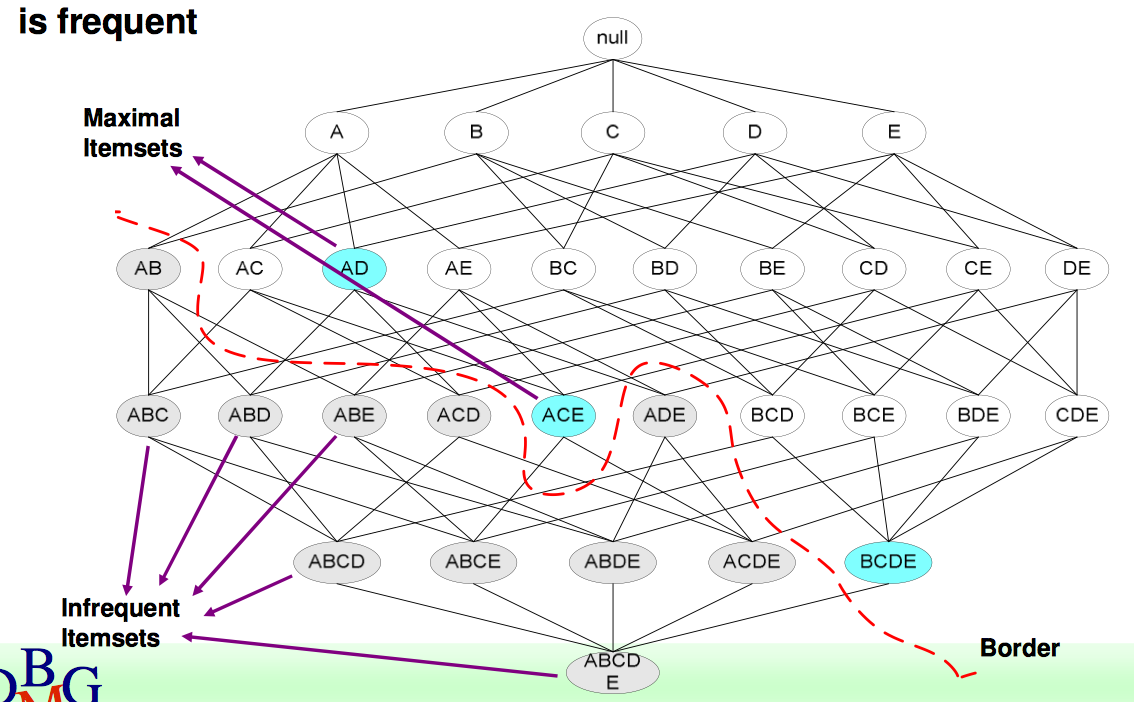
\includegraphics[width=\linewidth]{images/MFI.png}
  \caption{Maximal Frequent Itemset}
  \label{fig:MFI}
\end{figure}
In figure \ref{fig:MFI}, there are some highlighted elements AD, ACE and BCDE, they are MFI because there no other items longer then them with a sufficient frequency, infrequent, to be kept. They are useful because they can collapse a lot of informations. Some algorithms for generating it was developed.\\
Another important label for the itemsets is the \textbf{Closed Itemset} that occurs when if none of its immediate supersets has the same support as the itemset. In the case of table below:
\begin{figure}[H]
  \centering
  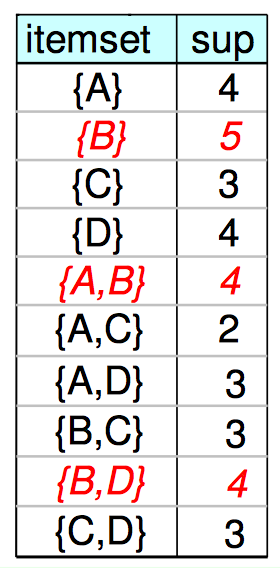
\includegraphics[width=0.2\linewidth]{images/CI.png}
  %\caption{Maximal Frequent Itemset}
  \label{fig:CI}
\end{figure}
The itemset \{A\} is not a CI because there is another itemset, longer, that include A with the same support of it and it's \{A,B\}, both for itemset \{D\} because it as the same support of \{D,B\} but is shorter. Is short word they are the longest itemset for a given length. The main difference respect the MFI is that they reduce the number of the itemsets but without losing information, you can generate all itemsets from them. Of course a Maximal is always a closed itemset.\\

One of the most hard choice is the selection of an appropriate \textit{minsup} threshold:
\begin{itemize}
  \item Too \textbf{high} \textit{minsup}: Itemset including rare but interesting items may be lost.
  \item Too \textbf{low} \textit{minsup}: Computionally very expensive, very large number of frequent itemsets.
\end{itemize}

A large number of pattern may be extracted, a solution is to rank patterns by their interestingness. For objective measures it useful to rank patterns based on statistics computed from data. There are also subjective measures that rank patterns according to user interpreatation.

\paragraph{Confidence measure} is the confidence always a reliable measure? No, this example will explain why:\\
In high school of 5000 students:
\begin{itemize}
  \item 3750 Eat Cereals
  \item 3000 Play basket
  \item 2000 Eat cereals and play basket
\end{itemize}
One of the extractable rule is: Play Basket $\Rightarrow$ Eat Cereals (Sup = 40\%, Conf = 66.7\%) and is misleading because eat cereals has sup 75\% (that is greater than 66.7\%). The problem is caused by the high frequency of rule head ("eat cereals"). Data used are:
\begin{center}
  \begin{tabular}{ |c|c|c|c| }
    \hline
    & \textbf{Basket} & \textbf{Not Basket} & \textbf{Total}\\
    \hline
    \hline
    Cereals & 2000 & 1750 & 3750\\
    \hline
    Not Cereals & 1000 & 250 & 1250\\
    \hline
    TOTAL & 3000 & 2000 & 5000\\
    \hline
  \end{tabular}
\end{center}
The solution to this problem is using another measurement called \textbf{Correlation} or \textbf{Lift}. The formula is:
\begin{equation}
  \begin{gathered}
    r: A \Rightarrow B\\
    Correlation = \frac{P(A,B)}{P(A)P(B)} = \frac{conf(r)}{sup(B)}
  \end{gathered}
\end{equation}
The result will be:
\begin{itemize}
  \item Statistical Independence: C = 1
  \item Positive Correlation: C > 1
  \item Negative Correlation: C < 1
\end{itemize}
Using the previous data the correlation become:
\begin{itemize}
  \item Play Basket $\Rightarrow$ Eat Cereals: C = 0.89 (Negative Correlations)
  \item Play Basket $\Rightarrow$ Not(Eat Cereals): C = 1.34
\end{itemize}

\subsection{Classification}
The classification is the process used to predict the class label. The process start from a training data, already classified by definition, the phase will generated a model. When unclassified data is passed through the model can be classified. A schema of classification process in figure \ref{fig:class}.
\begin{figure}[h!]
  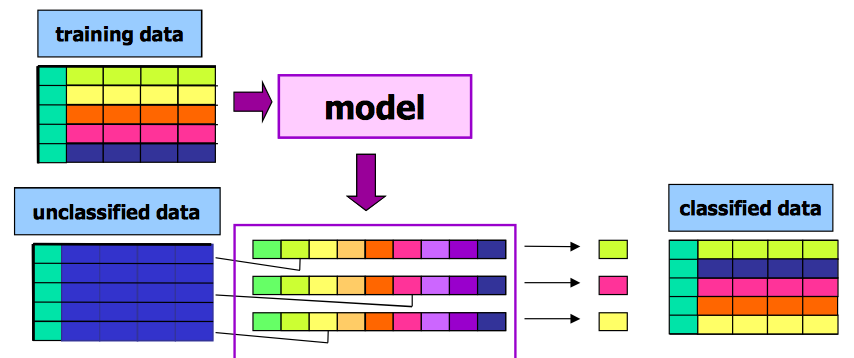
\includegraphics[width=\linewidth]{images/class.png}
  \caption{Classification process}
  \label{fig:class}
\end{figure}
There are several different approaches to the classification problem and they can be classified by its characteristics like accuracy, interpretability, scalability and noise/outliers management. Given a:
\begin{itemize}
  \item Collection of class labels
  \item Collection of data objects labelled with a class label
\end{itemize}
the goal is to find a descriptive profile of each class, which will allow the assignment of unlabeled objects to the appropriate class. After the training process is important to check the quality of the model, this is perfomed using a test set that is a collection of labeled data objects used to validate the calssification model, most of the time is directly direved from the training set.

\paragraph{Decision Trees} are the simplest method of classifing. The main structure is a tree where will flow some data to be checked by all different nodes to providing a classification. The process will end when, a block of data, reach a leaf (termination node, blue) where there is a classification class tag. This  An example in figure \ref{fig:dt}.
\begin{figure}[h!]
  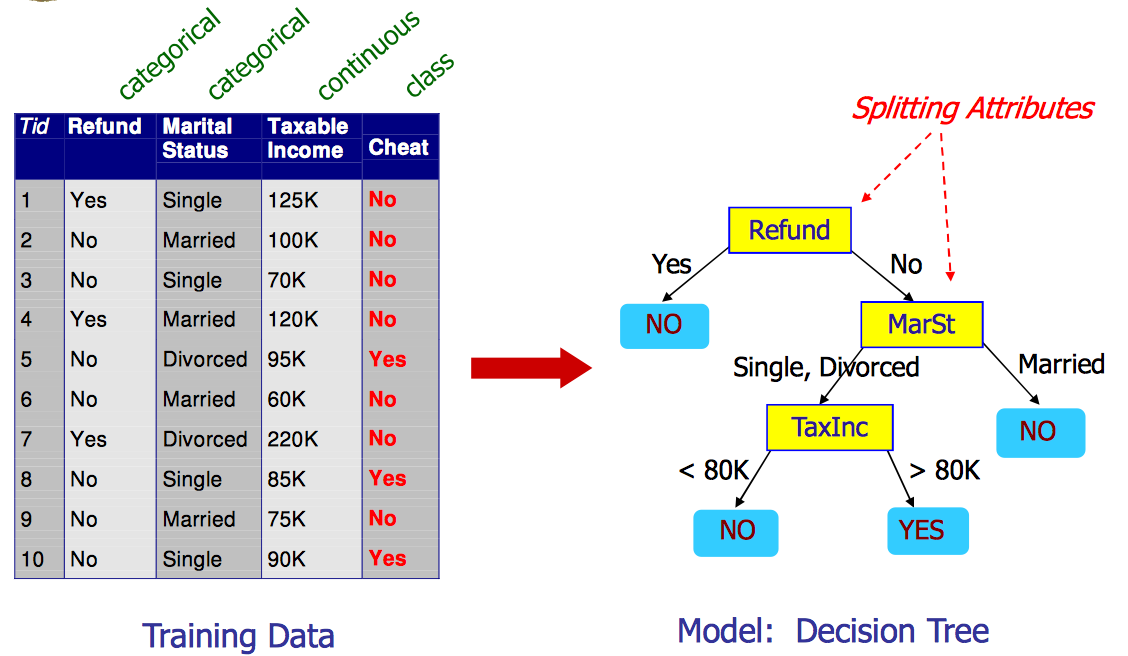
\includegraphics[width=\linewidth]{images/dt.png}
  \caption{From data to decision tree}
  \label{fig:dt}
\end{figure}
Each internal nodes is a splitting attribute, the number of exiting arch is correlated to the number of different value of the attributes, it could be binary or more.\\
The first algorith to build a decision trees is the Hunt's, nowadays the ID3 or C5.0 are more used. The flow is:
\begin{itemize}
  \item If $D_t$ contains records that belong to the same class $y_t$: Then is a leaf node labeled as $y_t$
  \item If $D_t$ contains records that belong to more than one class:
  \begin{enumerate}
    \item Select the "best" attribute A on which to split $D_t$ and label node t as A.
    \item Slipt $D_t$ into smaller subsets and recursively apply the procedure to each subset.
  \end{enumerate}
  \item If $D_t$ is an empty set: The t is a leaf node labeled as the default (majority) class, $y_d$.
\end{itemize}
All this flow is achieved with a greedy strategy, an exshaustive search will be superflous. The best attributes for the split is selected locally at each step (not a global optimum). The main problem are related to the kind of test condition, the selection of the best and the stopping condition.\\
The structure of test condition depends on attribute type that could be: nominal, ordinal and continuous and it depends on number of outgoing edges, 2 or multy-way split. The splitting can be of 2 different types, multy-way that it use as many partitions as distinct values, o binary that divide all the values in 2 subset or that have only teo distinct possible values. In case of continuos attributes there are different techniques:
\begin{itemize}
  \item Discretization: The subset are created using average, percentiles, clustering. They can be Static, defined at once the beginning, or dynamic, discretized during the tree iduction.
  \item Binary: Considering all possible splits and find the best cut (computationally intensive).
\end{itemize}
The selection of the best attribute is really important, our goal is to reach the end of the process, a leaf, as fast as possible, this is achieved by having a subset with only value of a single class. Using an attribute that not divide our data in "good" partitions, become unuseful, non-homogeneous and high degree of impurity (\textit{"Own car?"}). Defining good partition that collect a lot of data of a single class is important, more homogeneous, low degree of impurity (\textit{"Car type?"}). Also dividing is too much way is a waste of resources, not all attribute are profits for our tasks (\textit{"Student ID?"}). An example in figure \ref{fig:attr_sel}.
\begin{figure}[H]
  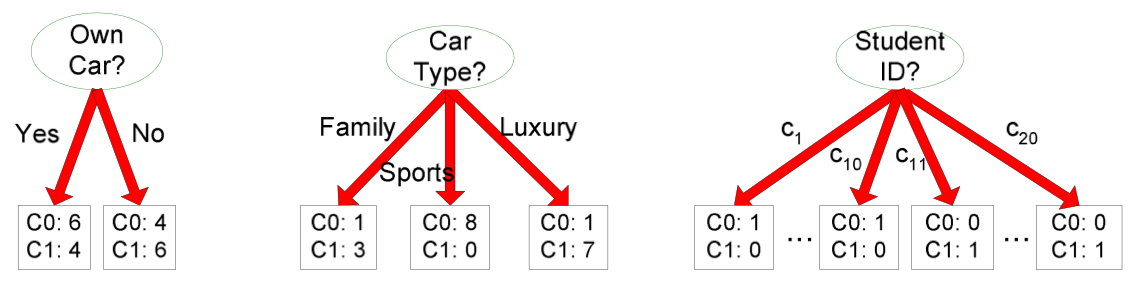
\includegraphics[width=\linewidth]{images/attr_sel.png}
  \caption{Attribute selection}
  \label{fig:attr_sel}
\end{figure}
How evaluate the impurity? The \textbf{gain} is the must used, it evaluate the density of the different classes before the splitting (M0), it apply two or more attribute and that it recompute the density after that applies (MA, MB), at the end it will compare the difference between the M0, MA and M0, MB and it will kept the purest one.\\
Another weel know index of purity is the \textbf{GINI}, that is, for a given node t:
\begin{equation}
  \begin{gathered}
    GINI(t) = 1 - \sum_{j} [p(j|t)]^{2}
  \end{gathered}
\end{equation}
The value is:
\begin{itemize}
  \item Maximum (1-1/\#ofClass): When the records are equally distributed among all classes, higher impurity degree.
  \item Minimum (0.0): When all records belong to one class, implying a lower impurity degree.
\end{itemize}
The idea is to divide the set in a weight way, a little but "more pure" class will have a greater weight, a big but "less pure" class will have a littler weight. All is achieved by using the formula:
\begin{equation}
  \begin{gathered}
    GINI_{split} = \sum_{i=1}^{k} \frac{n_i}{n} GINI(i)
  \end{gathered}
\end{equation}
where $n_i$ is the number of records at child i and n is the number of records at node p. In case of continuos attribute the system will start from the present value of that attribute and than it will try all the possibile splitting value to evaluate the best (GINI Index) solution, an example in figure .
\begin{figure}[H]
  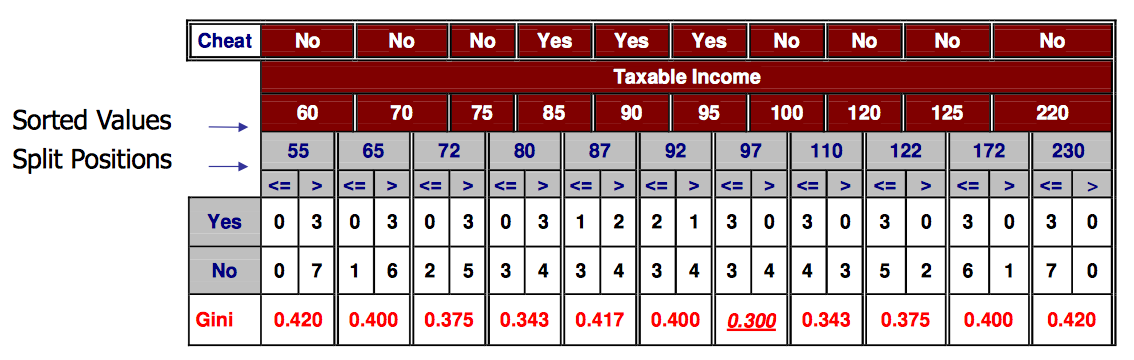
\includegraphics[width=\linewidth]{images/gini_cont.png}
  \caption{GINI index for continous attribute}
  \label{fig:gini_cont}
\end{figure}
Another well-know solution is the INFO (or Entropy impurity measure). The main difference is how this two index label the value. The entropy value is more "pessimistic" than the GINI one, because, for the same set, will give a worst quality of purity index for a class with a not-high impurity. In figure is easy to understand.
\begin{figure}[H]
  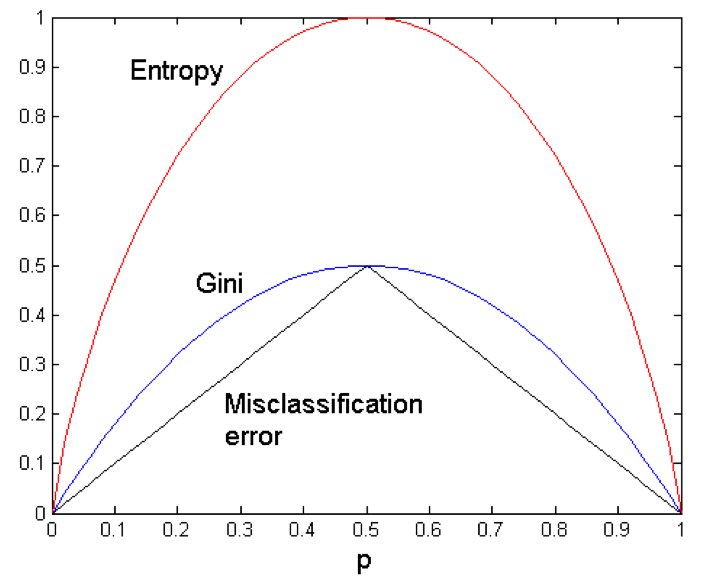
\includegraphics[width=\linewidth]{images/gini-info.png}
  \caption{GINI and INFO comparisons}
  \label{fig:gini-info}
\end{figure}

\paragraph{Stopping Criteria} the termination, for the Tree Induction, occurs in 3 different cases:
\begin{itemize}
  \item Stop exapanding a node when all the records belong to the same class.
  \item Stop exapanding a node when all the records have similar attribute values.
  \item Early termination.
\end{itemize}

\paragraph{Pro \& Cons} the decision tree based calssification have the advantages of:
\begin{itemize}
  \item Inexpensive to construct.
  \item Extremely fast at classifying unknow records.
  \item Easy to interpret for small-sized trees.
  \item Accuracy is comparable to other classification techniques for many simple data sets.
\end{itemize}
Instead, the main disadvantage is:
\begin{itemize}
  \item Accuracy mat be affected by missing data.
\end{itemize}
There are also some well-know issues related to this classification:
\begin{itemize}
  \item Under-over fitting.
  \item Missing values.
  \item Cost of classification.
\end{itemize}
The first issues occurs when the generated tree is too specific (high number of nodes) for the training set, it means that the error rate will increase during is application. The under fitting is the problem of having few nodes that implies a not very precise model. In figure \ref{fig:under_over} the underfitting border is when the blue curve become more stable (around 80 nodes).
\begin{figure}[H]
  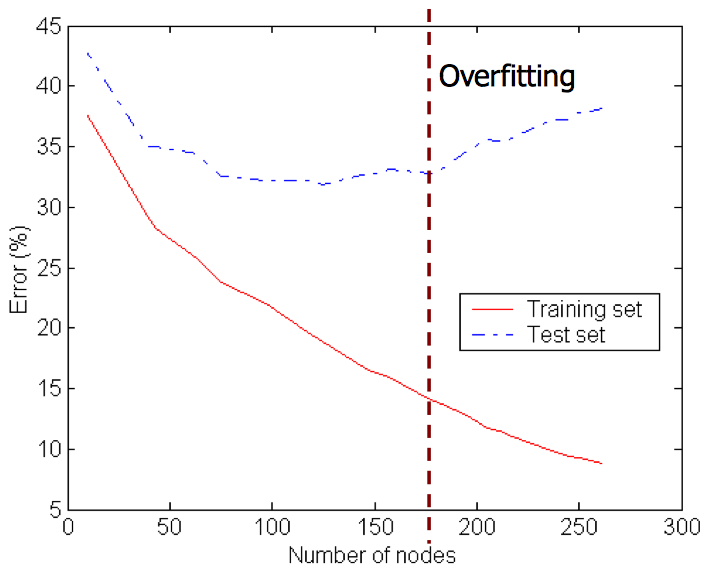
\includegraphics[width=\linewidth]{images/under_over.png}
  \caption{Under and over fitting problem}
  \label{fig:under_over}
\end{figure}
This problem is solved using the \textbf{pruning}. The PRE-pruning:
\begin{itemize}
  \item Stop the algorithm before it becomes a fully-grown tree.
  \item Typcal stopping conditions are:
  \begin{itemize}
    \item If all instances belong to the same class.
    \item If all the attribute values are the same.
  \end{itemize}
  \item Other more restrictive conditions:
  \begin{itemize}
    \item User defined threshold for the number of instances.
    \item If class distribution of instances are independent of the available features.
    \item If the exapanding will not improve the impurity measure.
  \end{itemize}
\end{itemize}
The POST-pruning solution:
\begin{itemize}
  \item Grow decision tree to its entirety.
  \item Trim the nodes of the decision tree in a bottom-up fashion.
  \item If generalization error improves after trimming, replace sub-tree by a leaf node.
  \item Class label of leaf node is determined from majority class of isntances in the sub-tree.
\end{itemize}
This is why the test set MUST NOT be the same of the training.\\
The handling of missing attribute values is important. They affect the tree decision construction in three ways:
\begin{itemize}
  \item How impurity measures are computed.
  \item How to distribute instance with missing value to child nodes.
  \item How a test instance with missing value is classified.
\end{itemize}

\paragraph{Search Strategy} Finding an optimal decision tree is NP-hard. The algorithm presented so far uses a greedy, top-down, recursive partitioning strategy to induce a reasonable solution. There are other strategies like bottom-up and bi-directional. The best situation where apply the decision tree is when the data is easy to be split in different class using boundaries parallels to the axes (\ref{fig:tree_good}). When the problem isn't solvable in this way is better to use different approaches (\ref{fig:tree_bad}).
\begin{figure}[h!]
  \centering
  \begin{minipage}{.45\textwidth}
    \centering
    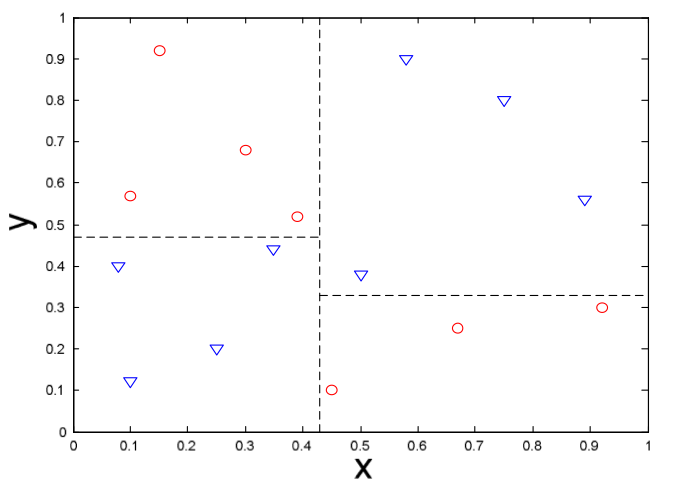
\includegraphics[width=\linewidth]{images/tree_good.png}
    \caption{Good use}
    \label{fig:tree_good}
  \end{minipage}\hfill
  \begin{minipage}{.45\textwidth}
    \centering
    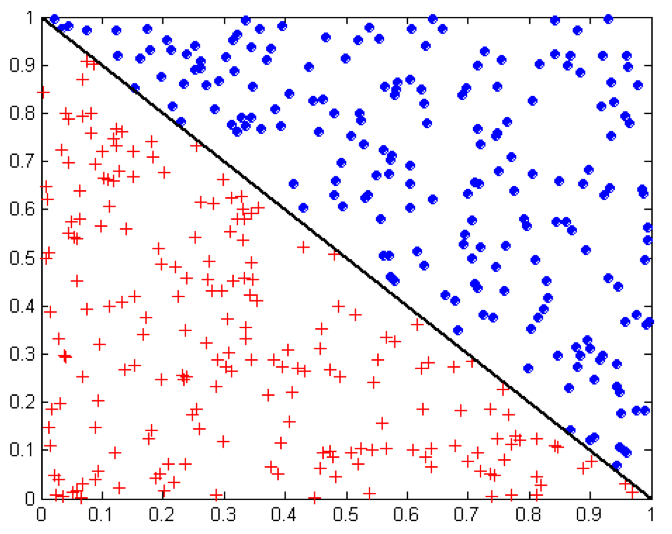
\includegraphics[width=\linewidth]{images/tree_bad.png}
    \caption{NOT Good use}
    \label{fig:tree_bad}
  \end{minipage}\hfill
\end{figure}

\paragraph{Rule Classification} Another possible technique is to classify records by using a collection of \textit{"if...then..."} rules. The result of applying this methods could be of three type:
\begin{itemize}
  \item Row matched by one rule.
  \item Row matched by more rules.
  \item Row not matched.
\end{itemize}
Rules can have two characteristics:
\begin{itemize}
  \item Mutually exclusive: Rules are independent of each other. Every record is covered by at most one rule.
  \item Exhaustive Coverage: If it accounts every possible combination of attribute values. Each record is covered by at least one rule.
\end{itemize}
Is possible to translate a Decision Tree to a Rule-based classification. The rules just created are ME and EC by definition because you can follow only one path at the time of the tree. Simplifying the rules could cause the lose of the ME, in these case a record may trigger more than one rule, the possible solutions are:
\begin{itemize}
  \item Ordered rule set.
  \item Unordered rule set - Use voting schemes.
\end{itemize}
When the lose is over the exhaustivity, having a record that not trigger any rules, the solution is using a default class (majority).\\
The advantages of this kind of classification are:
\begin{itemize}
  \item As highly expressive as decision tree.
  \item Easy to interpet.
  \item Easy to generate.
  \item Can classify new instances rapidly.
  \item Performance comparable to decision tree.
\end{itemize}

\paragraph{Associative Classification} This model is defined by means of association rules: (Condition) $\rightarrow$ y, where the body is an itemset. This scheme not look at one item at the time but to both (item, value) togheter, the difference is in the model generation:
\begin{itemize}
  \item Rule Selection \& Sorting: Based on support, confidence and correlation thresholds.
  \item Rule Pruning: Database coverage, the training set is covered by selecting topmost rules according to previous sort.
\end{itemize}
Some PRO of this approach are:
\begin{itemize}
  \item Interpretable model.
  \item Higher accuracy that DT (correlation among attributes is considered).
  \item Efficient classification.
  \item Enaffected by missing data.
  \item Good scalability in the training set size.
\end{itemize}
The WEAK point are:
\begin{itemize}
  \item Rule generation may be slow.
  \item Reduced scalability in the number of attributes.
\end{itemize}

\paragraph{Neural Networks} They are inspired by the structure of the human brain, with elaboration units (neurons) and connection network (synapses). The structure is simplyfied in figure \ref{fig:str_net}.
\begin{figure}[H]
  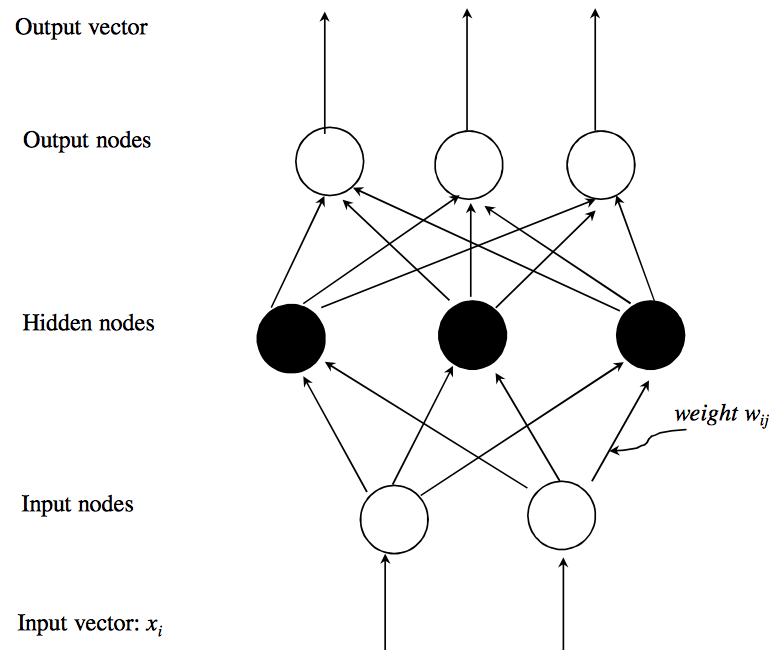
\includegraphics[width=\linewidth]{images/str_net.png}
  \caption{Structure of a neural network}
  \label{fig:str_net}
\end{figure}
The general structure of a neurons use an input and a weight vectors to generate a weighted sum (scalar product). After the addition of an offset it compute a function and then it provides the output values.\\
The model of the networks is based on all the weight and all the offset value of each node.\\
The training is based on an iterative approach. The base algorithm is:
\begin{enumerate}
  \item Assign random values to weights and offsets.
  \item Process instances in the training set one at a time:
  \begin{enumerate}
    \item For each neuron, compute the result when applying weights, offset and activation function for the instance.
    \item Forward propagation until the output is computed.
    \item Compare the computed output with the expected output, and evaluate error.
    \item Backpropagation of the error, by updating weights and offset for each neuron.
  \end{enumerate}
\end{enumerate}
The process ends when:
\begin{itemize}
  \item The \% of accuracy above a given threshold.
  \item The \% of parameter variation (error) below a given thereshold.
  \item The maximum number of epochs (number of times training sets parsed) is reached.
\end{itemize}
These system has some strong points:
\begin{itemize}
  \item High Accuracy.
  \item Robust to noise and outliers.
  \item Supports both discrete and continous output.
  \item Efficient during classification.
\end{itemize}
The main weak points insted:
\begin{itemize}
  \item Long training time: Weakly scalable in training data size. Complex configuration.
  \item Not interpretable model: Application domain knowledge cannot be exploited in the model.
\end{itemize}

\paragraph{Bayesian Classification} Is really different from the previous methods explained. Is based on the Bayes theorem:
\begin{equation}
  \begin{gathered}
    P(C,X) = P(C|X)P(X) = P(X|C)P(C)\\
    P(C|X) = \frac{P(X|C)P(C)}{P(X)}
  \end{gathered}
\end{equation}
The approch is:
\begin{itemize}
  \item Let the class attribute and all data attributes be random variables (C = Any Class, $X = <x_1,...,x_k>$).
  \item Classification:
  \begin{itemize}
    \item Compute $P(C|X)$ for all classes (Probability that record X belongs to C).
    \item Assign X to the class with the \textit{\textbf{maximal}} $P(C|X)$.
  \end{itemize}
\end{itemize}
The computeation is achieved using the Bayes theorem, where P(C) is A Priori probability, without valculating the fraction (we not need the probability but only the highest value). The problem is how to calculate the $P(X|C)$, i.e $P(x_1,...,x_k|C)$ and it was solved using a Naïve hypothesis: All attributes are \textbf{statistical indipendent}, of course this is not always true and it can affect the model quality.\\
For example, strating from the data below:
\begin{figure}[H]
  \centering
  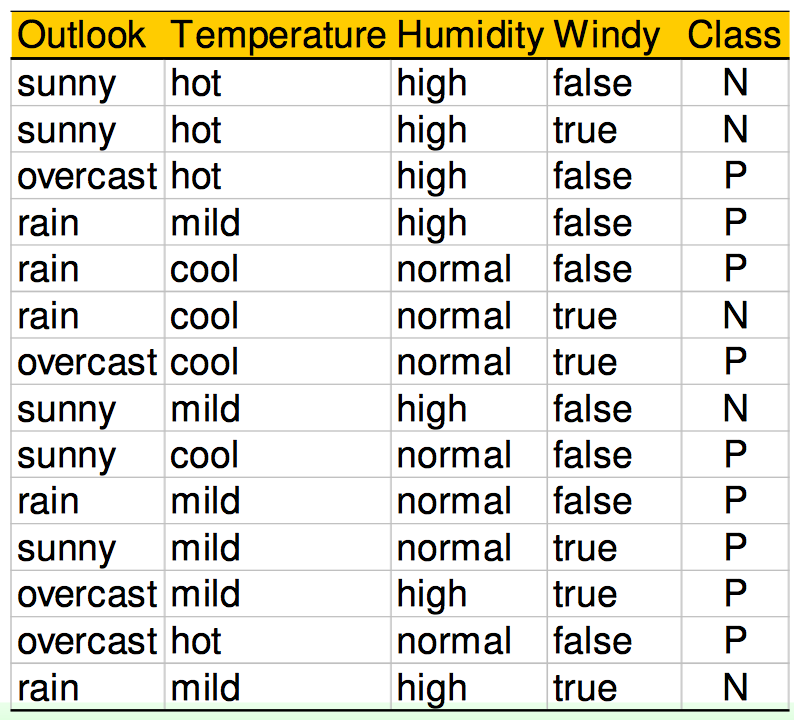
\includegraphics[width=0.8\linewidth]{images/bay_data.png}
  %\caption{Data for example}
  \label{fig:bay_data}
\end{figure}
after the computation of all possibilities below:
\begin{figure}[H]
  \centering
  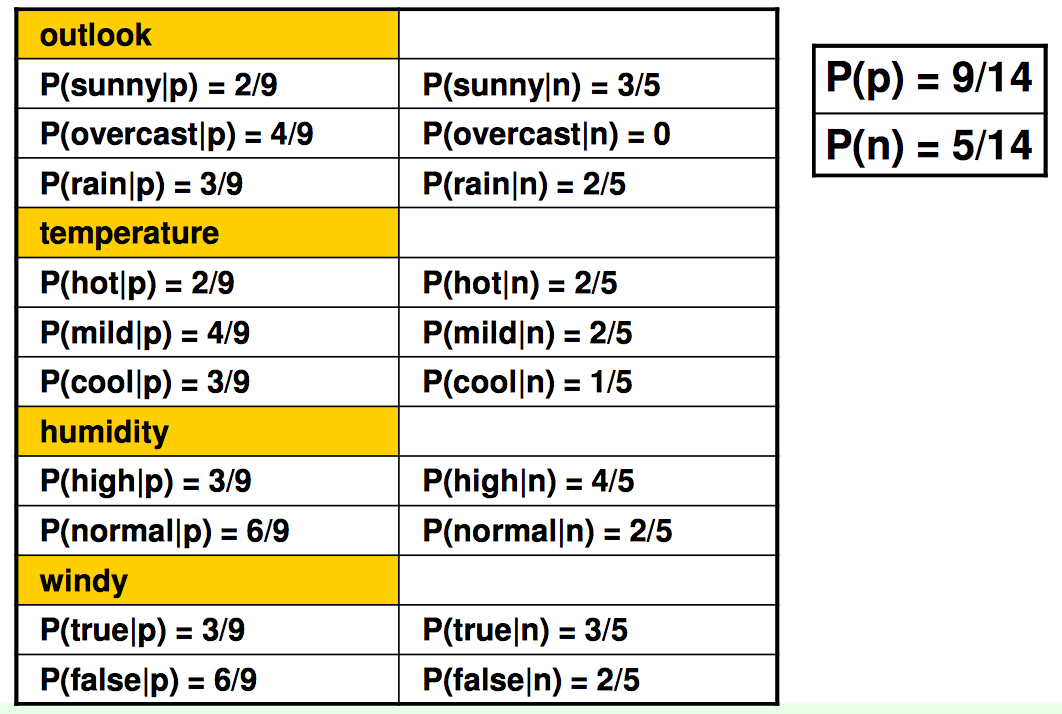
\includegraphics[width=0.8\linewidth]{images/bay_comp.png}
  %\caption{Data for example}
  \label{fig:bay_comp}
\end{figure}
When a new data ($X = <rain, hot, high, false>$) to be labeled is insert the flow will compute this value:
\begin{itemize}
  \item For class \textit{p}: $P(X|p)P(p) = 3/9*2/9*3/9*6/9*9/14 = 0.010582$
  \item For class \textit{n}: $P(X|n)P(n) = 2/5*2/5*4/5*2/5*5/14 = \textbf{0.018286}$
\end{itemize}

\subsection{Clustering Fundamentals}
\textit{What is Cluster Analysis?} Finding groups of objects such that the objects in a group will be similar (or related) to one another and different from (or unrelated to) objects in other groups.
\begin{figure}[H]
  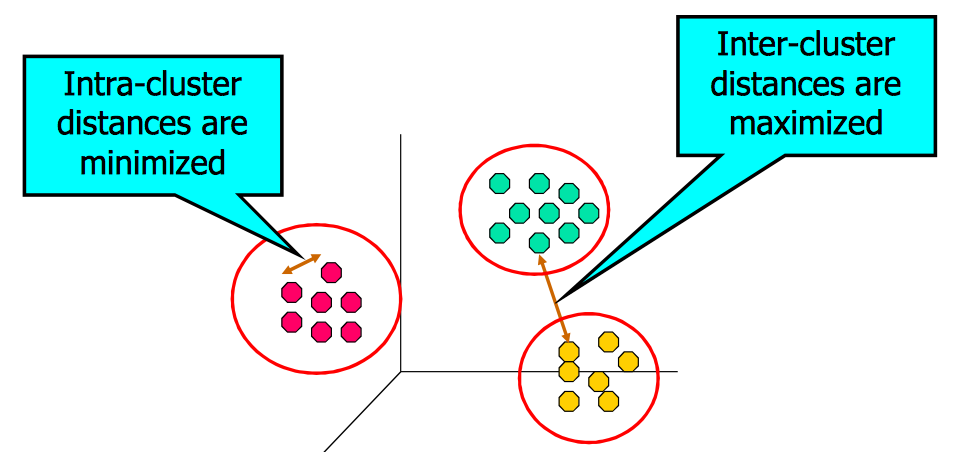
\includegraphics[width=\linewidth]{images/clustering.png}
  \caption{The clustering ideas}
  \label{fig:clustering}
\end{figure}
This is a data-mining technique not-supervisioned, it means that, respect the classification, it not require the class tag.
The main applications of this analysis are:
\begin{itemize}
  \item \textbf{Understanding}: Group related documents for browsing, group of genes or proteins with similar functionality, etc...
  \item \textbf{Summarization}: Reduce the size of large data sets.
\end{itemize}
The problem of clustering is related to its definition that can be ambiguous, the best cluster division is always related to the request of the problem, there isn't a always-best solution.\\
\paragraph{Type of cluster} A clustering is a set of clusters, there are two main type of cluster:
\begin{itemize}
  \item \textbf{Partitional}: A division data objects into non-overlapping subsets (cluster) such that data object is in exactly one subset.
  \item \textbf{Hierarchical}: A set of nested cluster organized as hierarchical tree.
\end{itemize}

\begin{figure}[h!]
  \centering
  \begin{minipage}{.45\textwidth}
    \centering
    \includegraphics[width=\linewidth]{images/part.png}
    \caption{Partitional Cluster}
    \label{fig:part}
  \end{minipage}\hfill
  \begin{minipage}{.45\textwidth}
    \centering
    \includegraphics[width=\linewidth]{images/hier.png}
    \caption{Hierarchical Cluster}
    \label{fig:hier}
  \end{minipage}\hfill
\end{figure}

Other distrinctions between sets of clusters are:
\begin{itemize}
  \item Exclusive vs Non-exclusive: In eXclusive, point not belong to multiple clusters.
  \item Fuzzy vs non-fuzzy: In fuzzy, a point belongs to every cluster with some weight (0<w<1).
  \item Partial vs Complete: In some cases, we only want cluster some of the data.
  \item Heterogeneous vs homogeneous: Cluster of widely sizes, shapes and densisties.
\end{itemize}

The types can be also distrincted by its shapes:\\
In a \textbf{Well Separated} cluster the point are distribuited such that any point in a cluster is closer (or more similar) to every other point in the cluster than to any point not in the cluster (figure \ref{fig:we_sep}).
\textbf{Center-based} means that an objects in a cluster is more similar to its center than to the center of any other cluster. The center can be found with the average of all point in the cluster (\textit{centroid}, it may not be a record), or with the most "representative" point (\textit{medoid}) of a cluster (figure \ref{fig:ce_ba}).
\begin{figure}[h!]
  \centering
  \begin{minipage}{.45\textwidth}
    \centering
    \includegraphics[width=\linewidth]{images/we_sep.png}
    \caption{Well Separated}
    \label{fig:we_sep}
  \end{minipage}\hfill
  \begin{minipage}{.45\textwidth}
    \centering
    \includegraphics[width=\linewidth]{images/ce_ba.png}
    \caption{Center-based}
    \label{fig:ce_ba}
  \end{minipage}\hfill
\end{figure}
Another type is the \textbf{Contiguity-based} that collect closer point to one or more other points in the cluster than to any point not in the cluster, they can have strange shapes (figure \ref{fig:cont}). In the \textbf{Density-based} the clusters are identified by high-density region of point, which are separated by low-densisty regions. The \textbf{Share Property} or conceptual clusters shares some common property or represent a particular concept (figure \ref{fig:share}).
\begin{figure}[h!]
  \centering
  \begin{minipage}{.45\textwidth}
    \centering
    \includegraphics[width=\linewidth]{images/cont.png}
    \caption{Contiguity}
    \label{fig:cont}
  \end{minipage}\hfill
  \begin{minipage}{.45\textwidth}
    \centering
    \includegraphics[width=\linewidth]{images/share.png}
    \caption{Share Property}
    \label{fig:share}
  \end{minipage}\hfill
\end{figure}

\paragraph{Algorithms} One of the most important is the \textbf{K-menas}. Used for partitional clusters, it associate each cluster with a centroid and each point is assigned to the cluster with the closest centroid. The number of cluster must be choose by the user. After the centroid choice is necessary to recompute the centroid. The algorithm is really simple.\\
The initial centroids are often chosen randomly, it means that the clusters produced vary from one run to another. The distance can be evaluated in different ways, Euclidean, cosine, similarity, etc... The k-means will converge in the first few iterations (figure \ref{fig:kmeansConve}). The complexity is O(n*K*I*d), where n = \#ofPoints, K = \#ofClusters, I = \#ofIterations and d = \#ofAttributes.
\begin{figure}[H]
  \includegraphics[width=\linewidth]{images/kmeansConve.png}
  \caption{Convergence of K-means}
  \label{fig:kmeansConve}
\end{figure}
In situations of 10-15 dimensions is impossible to evaluated the "goodness" of a solutions, this can be achieved using \textbf{SSE} or Sum of Squared Error. For each point, the error is the distance to the nearest cluster. The formula is:
\begin{equation}
  \begin{gathered}
    SSE = \sum^{K}_{i=1} \sum_{x \in C_i} dist^2(m_i, x)
  \end{gathered}
\end{equation}
\textit{x} is a data point and $m_i$ is the representative point for cluster its cluster $C_i$. Given more cluster, we can choose the one with the smallest error. One way to reduce SSE is to increase K.\\
In some cases the basic k-means algorithm can yeild empty clusters, is important to handling it. Some solutions are:
\begin{itemize}
  \item Choose the point that contributes most to SSE.
  \item Choose a point from the cluster with the highest SSE.
  \item If there are several empty clusters, the above can be repeated several times.
\end{itemize}
Is possible to increase the quality of the system with some pre-processing operation like:
\begin{itemize}
  \item Normalization (Always need).
  \item Eliminate Outliers.
\end{itemize}
There also some post-processing operations:
\begin{itemize}
  \item Eliminate small cluster that may represent outliers.
  \item Split 'loose' clusters (high SSE).
  \item Merge clusters that are 'close' and that have relatively low SSE.
  \item Can use these step during the clustering process.
\end{itemize}

The \textbf{bisecting K-means} is an alternative to the k-means, it applies the normal k-means by splitting a cluster,  the worst one (high SSE), in 2 cluster. These step are iterated many times until the number of cluster is K. Normally this solution give better results than the normal k-means.\\
Both k-means solution has problem when clusters are of differing in size (\ref{fig:size}), densities (\ref{fig:dens}) or non-globular shapes (\ref{fig:shape}), also outliers can cause problems.
\begin{figure}[h!]
  \includegraphics[width=\linewidth]{images/size.png}
  \caption{Size problem}
  \label{fig:size}
\end{figure}
\begin{figure}[h!]
  \includegraphics[width=\linewidth]{images/dens.png}
  \caption{Density problem}
  \label{fig:dens}
\end{figure}
\begin{figure}[h!]
  \includegraphics[width=\linewidth]{images/shape.png}
  \caption{Shape problem}
  \label{fig:shape}
\end{figure}
One solution is to use an high number of K and then merge it in a post-processing phase.

The \textbf{hierarchical Clustering} algorithms produces a set of nested clusters organized as a hierarchical tree. They can be visualized as a dendrogram (a tree like diagram that records the sequences of merges or splits). They can be created bottom-up or top-down. They don't have to assume any particular number of clusters. Two main types:
\begin{itemize}
  \item Agglomerative: Points as individual clusters. Each step, merge the closest pair of clusters until only one cluster left.
  \item Divisive: Start with one, all-inclusive cluster. Each step, split a cluster until each cluster contains a point.
\end{itemize}
Since in the intermediate steps we will have only clusters, is necessary to have measurement for distance between points, already studied in classification section, and between clusters. All the computation is made with a proximity matrix.\\
There are 5 main measure, the first 3 are computing all couples combination between two cluster and than select the MIN, MAX or Average distance between them. Another possibilities is to compute the distance between centroids.  All these possibilities are done to fill the proximity matrix.\\
The advantage of the \textbf{MIN} is that it can handle non-elliptical shapes, the limitations is that is sensitive to noise and outliers. Instead, the \textbf{MAX} is less susceptible to noise and outliers, but it tends to break large clusters (like K-means).\\
The most expensive step is the computation of the matrix, the space complexity is $O(N^2)$, where N is the number of points, the time complexity is $O(N^3)$.\\

Another algorithm is the \textbf{DBSCAN} that is density-based, it's good to check outliers and noise. The density is computed like the number of points eithin a specified radius $\epsilon$. The points are classified, given $\epsilon$ and $minPts$, with three label:
\begin{itemize}
  \item \textbf{Core}: If it has more than a \textit{minPts} within $\epsilon$.
  \item \textbf{Border}: Fewer than \textit{minPts} in $\epsilon$ but near to a core point.
  \item \textbf{Noise}: Any point not a Border or a Core ones (added to the cluster 0).
\end{itemize}
An example in figure \ref{fig:dbscan}.
The implementation is not too easy, the pseudo code is the following:
\begin{figure}[H]
  \centering
  \includegraphics[width=0.8\linewidth]{images/dbscan_pseudo.png}
  %\caption{DBSCAN example}
  \label{fig:dbscan_pseudo}
\end{figure}
\begin{figure}[h!]
  \centering
  \includegraphics[width=0.8\linewidth]{images/dbscan.png}
  \caption{DBSCAN example}
  \label{fig:dbscan}
\end{figure}
The strenght of the DBSCAN is that is really resistant to noise and it can hadle clusters of different shapes and sizes. It not works well in case of varying densisties and high-dimensional data. The first problem can be solved performing two iterations of the algorithm, in the first one you'll find the high-dense clusters, in the second one the less-dense.\\
\textit{How determing $\epsilon$ and minPts?} The ideas is to plot a graph with sorted distance of every point to its $k^{th}$ nearest neighbor. This because for points in a cluster, their $k^{th}$ nearest neighbors are at roughly the same distance, instead the noise points are farther. Normally the value of k is choose at the knee of the curve (around 10 in figure \ref{fig:knee}), in case of multiple knees it means that there are different density zones.
\begin{figure}[H]
  \centering
  \includegraphics[width=0.8\linewidth]{images/knee.png}
  \caption{Example of graph for determining $\epsilon$ and \textit{minPts}}
  \label{fig:knee}
\end{figure}

\paragraph{Cluster Validity} this is the most difficult tasks. Some numerical measure can be exploited to evaluate the "goodness" of the solution. They are classified in two main classes:
\begin{itemize}
  \item External Index: Used to measure the extent to which cluster labels match externally supplied class labels, like a training sets (entropy, purity).
  \item Internal Index: Used to measure the goodness of a clustering structure without respect to external information (SSE, cohesion (how near), separation (how far), rand-index).
\end{itemize}

\bigskip
``The validation of clustering structures is the most difficult and frustrating part of cluster analysis.\\
Without a strong effort in this direction, cluster analysis will remain a black art accessible only to those true believers who have experience and great courage.''\\
\rightline{{\rm --- \textbf{Jain and Dubes}, Algorithms for Clustering Data}}


%--------------------------------------------------------------------------------------------------------
%--------------------------------------------------------------------------------------------------------
%--------------------------------------------------------------------------------------------------------
\clearpage
\section{Beyond Relational Databases}
\subsection{Introduction}
The first NoSQL databases was developed around 1998. The main difference are three:
\begin{itemize}
  \item No joins: Complex and unuseful in some cases.
  \item Schema-less: No tables, implicit schema.
  \item Horizontal scalability: Adding machines not require to stop.
\end{itemize}
In this kind of systems the table are substituted with \textbf{specialized storage} solutions like document-based, key-value pairs, graph databases and columnar storage. Removing the scemas constraints allows better option for managing dynamic changing documents, semi-structured or un-structured data. The advantages of an Horizontal scalability is that sufficient to add a server to your pool in order to reduce the load. In the classic system the only solution is to increase the power of the system. The main drawbacks is that there isn't a standardized language for the managing, each system has is own language. The old complex joins are now solved with non standard interfaces. The SQL system are better for managing flat and structured data, the NoSQL are better for complex (e.g. Hierarchical) data like JSON and XML. Some example of NoSQL software are \textbf{MongoDB}, BigTable, Redis, Cassandra, HBase and CouchDB. In some cases NoSQL software developer, like the Mongo ones, have introduct some "more SQL" feature to its build to better fit some problem.
\subsection{Structure}
These new kind of system have also introduced new types of data structures, the most important are in figure \ref{fig:tnosql}.
\begin{figure}[H]
  \includegraphics[width=\linewidth]{images/tnosql.png}
  \caption{Types of NoSQL databases}
  \label{fig:tnosql}
\end{figure}
The first type is the \textbf{key-value} is:
\begin{itemize}
  \item \textbf{Simplest} data stores.
  \item Macth keys with value.
  \item No Structure.
  \item \textbf{Great performance}.
  \item Easy scalable.
  \item Very fast.
  \item Examples: Redis, Riak, Memcached (used to solve FB problem).
\end{itemize}
The second one is the \textbf{column-oriented} databases that are:
\begin{itemize}
  \item Store data in columnar format.
  \item A column is a (complex) attribute.
  \item Key-value pairs stored and retrived on key in a parallel system (similar to indices).
  \item Rows can be constructed from cloumn values.
  \item Column stores can produce row output (\textbf{tables}).
  \item Completely transparent to application.
  \item Example: Cassandra, HBase, Hypertable, AMZ DynamoDB.
\end{itemize}
Another structure is the \textbf{graph}, the main feature are:
\begin{itemize}
  \item Based on graph theory.
  \item Made up by \textbf{Vertex} and \textbf{Edges}.
  \item Used to store information about networks.
  \item Good fit for several real world application.
  \item Examples: Ne04J, Infinite Graph, OrientDB.
\end{itemize}
The last structure is the \textbf{document} ones, where document means complex, that is:
\begin{itemize}
  \item Database stores and retives documents.
  \item Keys are mapped to documents.
  \item Documents are self-describing (\textbf{attribute=value}).
  \item Has hierarchical-tree nested data structures (e.g. Maps, lists, datetime, ...)
  \item \textbf{Heterogeneous} nature of documents.
  \item Examples: \textbf{MongoDB}, CouchDB, RavenDB.
\end{itemize}

\subsection{NoSQL example: CouchDB}
The CouchDB is good to be studied because is kept is soul entirely on the NoSQL side respect other software, is a Pure NoSQL database.\\
CouchDB is a document-oriented database can be queried and indexed in \textbf{MapReduce} fashion, it offers incremental \textbf{replication} with bi-directional conflict detection and resolution. Is written in Erlang, a robust functional programming language ideal for building concurrent \textbf{distributed systems}. Erlang allows for a flexible design that is easily scalable and readily extensible. Is also RESTful JSON API that allows access from any environment that permit HTTP request, it don't need a client.
\paragraph{MapReduce} is a scalable distributed programming model to process Big Data. The first analisys over these model come from Google in 2004, they have try to change the point of view trying to passe the code to the node ehere the data is stored and not get all the data to the central code node. It consist in two function:
\begin{itemize}
  \item \textbf{Map}:
  \begin{itemize}
    \item Process each record (document) indipendently.
    \item Return a list of key-value pairs.
  \end{itemize}
  \item \textbf{Reduce} (optional):
  \begin{itemize}
    \item Reduce the list of key-value returned by the map to a single value (it can be a complex value such as a map).
  \end{itemize}
\end{itemize}
The map function is called one document by one and it get back a key, that index in a sorted way the result, and the value itself. Performing a function like this:
\begin{lstlisting}[frame=single]
  Function(doc) {
    emit(doc.exam, doc.mark);
  }
\end{lstlisting}
The result take the value of the DB on the left and transform it to the table on the right of the figure
\ref{fig:map}.
\begin{figure}[H]
  \includegraphics[width=\linewidth]{images/map.png}
  \caption{Map function example}
  \label{fig:map}
\end{figure}
The key can be more complex adding, for example the accademy year. Also the value can be complex adding the CFU for computing later an weighted average and so on.\\
The reduce function perform operations over the value returned by the map function. The most simple SQL-equivalent operations performed by means of reducers are "group by" aggregations, but with more more powerful functions to be implemented. It also possible to perform reduce over already reduced sets. For example, using this function:

\begin{lstlisting}[frame=single]
  Function(key, value) {
    S = sum(values);
    N = len(values);
    AVG = S/N;

    return AVG;
  }
\end{lstlisting}

The output start from the left table and perform operations to return a structure like the right one of the figure \ref{fig:reduce}.
\begin{figure}[H]
  \includegraphics[width=\linewidth]{images/reduce.png}
  \caption{Reduce function example}
  \label{fig:reduce}
\end{figure}
as you can see all the exams are grouped and there is no difference between the same exam created with the exam name like keys. If this operations is computed over a starting table with (ExamName, AccYear) like keys the result will be with exams grouped by name and accamedic year; the result is similar to the \textit{GROUP BY Exam, AYear}. One of the most important feature of this system is the parallelization capabilities, in figure \ref{fig:mp_par} an example of how the result will be computed with more nodes with data.
\begin{figure}[H]
  \includegraphics[width=\linewidth]{images/mp_par.png}
  \caption{Parallel workflow example}
  \label{fig:mp_par}
\end{figure}

\subsection{Replication}
The replication try to keep the same data, portions of it, in different places, like local and/or remote servers, clusters, data centers. The main goals are:
\begin{itemize}
  \item Redundancy helps surviving failures (availability).
  \item Better performance.
\end{itemize}
To achieve this feature the are two possible solutions.
\paragraph{Master-Slave} this first solution implement a \textit{master} server that takes all the writes, updates and insert and some \textit{slaves} servers that take all the reads (they can't write). This means only a read scalability and the master become a single point of failure. In the case of CouchDB also the Master-Master replications can be implemented.
\paragraph{Synchronous replication} is a different solution, the master will waits the commit of all slaves, before commiting. This is similar to the 2-phase commit in RDB. It could be performance killer! A treade-oof could be wait only for a subset (majority) of slaves before commit.
\paragraph{Asynchronous replication} have a master that commit all operations without waiting the slaves. Each slaves independently fetchs update from master, which may fail...
\begin{itemize}
  \item If no slave has replicated, the you've lost the data commited to the master.
  \item If some slaves have replicated and some haven't, then you have to reconcile.
\end{itemize}
This is a faster but unreliable solution.

\subsection{Distributed databases}
Different autonomous machines, working together to manage the same dataset. There are 3 typical problems in distributed databases:
\begin{itemize}
  \item \textbf{Consistency}: All distributed DB provide the same data to the application.
  \item \textbf{Availability}: Database failures (e.g. Master Node) do not prevent survivors from continuing to operate.
  \item \textbf{Partition} tolerance: The system continues to operate despite arbitrary message loss, when connectivity failures causes network partitions.
\end{itemize}

\paragraph{CAP Theorem} also know as Brewer's theorem, states that it is impossible for a distributed system to simultaneously provide all three of the previous guarantees. It becomes a theorem in the 2002. A representation in figure
\begin{figure}[h!]
  \centering
  \includegraphics[width=0.7\linewidth]{images/cap.png}
  \caption{Cap theorem chart}
  \label{fig:cap}
\end{figure}
In general is not to difficult to be understand. Allowing at least one node to update state will cause the nodes to become inconsistent, thus forfeiting C. If the choice is to preserve consistency, one side of the partition must act as if it is unavailable, thus forfeiting A. Only when no network partition exist, is it possible to preserve both consistency and availability, thereby forfeiting P.\\
The general delief is that for wide-area system, deesigners cannot forfeit P and therefore have a difficult choice between C and A. This is because is impossible to have a distributed systems without allowing network partition in case of failures, therefore is not still a distributed system.\\
The \textbf{CP} solutions guarantee the consistency of the data, it similar to the 2-phase locking where an agreement is needed to commit the operations. This is means that everything is been blocked since all response have comed back. For example, guaranteeing C allows to show the correct availability for a product to all the Amazon's costumers. It can be really expensive because is better to manage situation where more people have bought only one item, rather than not sell it. In this case \textbf{AP} (a.k.a best effort) become a good solution, this sacrifice the consistency but it can guarantee a good service, even though the system as a shole has benn broken up into incommunicable regions (partitions). This situations not means that the global consistency is always broken, it only means that is \textbf{can't be guarantee all the time}.

\bigskip
``Each node in a system should be able to make decisions purely based on local state. If you need to do something under high load with failures occurring and you need to reach agreement, you’re lost. If you’re concerned about scalability, any algorithm that forces you to run agreement will eventually become your bottleneck. Take that as a given.''\\
\rightline{{\rm --- \textbf{Werner Vogels}, Amazon CTO and Vice President}}
\bigskip

In general the the "2 of 3" view is misleading on several fronts. First, because partitions are rare, there is a little reason to forfeit C or A when the system is not partitioned. Second, the choice between C and A can occur many times within the same system at very fine granularity; not only can subsystem make different choices, but the choice can change according to the operation or even the specific data or user involved. Finally, all three properties are more continuous that binary. Availability is obviously continous from 0 to 100 percent, but there are also many levels of consistency, and even partitions have nuances.

\paragraph{BASE} this kind of systems prefer to use a different properties respect the ACID one. The BASE consists in:
\begin{itemize}
  \item \textbf{Basically Available}: The system provides availability, in terms of the CAP theorem.
  \item \textbf{Soft state}: Indicates that the state of the system may change over time, even without input, because of the eventual consistency model.
  \item \textbf{Eventual consustency}: Indicates that the system will become consistenct over time, given that the system doesn't receive input during that time.
\end{itemize}

\subsection{Conflict resolution}
Supposing that there are two customers, A and B. A books a hotel room, the last available. B does the same, on a different node of the system, which was not consistent. The hotel room document is affected by two conflicting updates. The applications should solve the conflict with custom logic (it's a business decision). The DB can:
\begin{itemize}
  \item Detect the conflict.
  \item Provide a local solution, e.g., latest version is saved as the winning version.
\end{itemize}
In CouchDB is guarantee that each instance that sees the same conflict comes up with \textbf{same winning} and losing revisions. It does so by running a deterministic algorithm to pick the winner:
\begin{itemize}
  \item The revision with the longest revision history list becomes the winning revision.
  \item If they are the same, the \_rev cvalues are compared is ASCII sort order, and the highest wins.
\end{itemize}

\subsection{HTTP RESTful API}
This are an important characteristics of this systems. It's really easy to get a document, you only need to use your browser and write its url, e.g., \textit{http://localhost:5984/test/some\_doc\_id}. And so on. All operations have a proper procedure to be used, but this is beyond the pourpose of this course.

\subsection{Conclusions} If you're building an app today, then there might be a need for using two or more databases at the same time, this is because there isn't a solutions that fits everything you need, some times using a more structured ways is preferred, some times is not usable. In general the choice depends on your needs, and it's probably that not just one DB can solve your problem.

%--------------------------------------------------------------------------------------------------------
%--------------------------------------------------------------------------------------------------------
%--------------------------------------------------------------------------------------------------------
\clearpage
\section{Big Data} % 8/12/17
\subsection{Introduction}
Big Data is about Seach, lot of bytes, storage and analytics. Big data not makes magic and it could give bad result if not performed well. Where get all this data? Of course from the web, mobile, social, sensors from healt to scientific, log files, IoT, and so on...\\
One of the most common definition of BD is: "\textit{Data whose scale, diversity and complexity require new architectures, techniques, algorithms and analytics to manage it and extract value and hidden knowledge from it}".

\paragraph{BigData Vs} There are some know Vs regarding BD, they are:
\begin{itemize}
  \item Volume: Scale of data
  \item Variety: Different forms of data.
  \item Velocity: Analysis of streaming data.
\end{itemize}
Other 2 important think were added during times:
\begin{itemize}
  \item Veracity: Uncertainty of data.
  \item Value: Exploit information provided by data.
\end{itemize}

The volume of our data growth really really faster, we speaking now of thousant of terabytes normally. They increase in exponential way, the forecast say that in 2020 will reach decines of petabytes. The variety of this kind of data is impressive, from numerical to image, audio, text, video and so on... A single application may generate many different formats. The data could be fast as you can't store it, like the stream, you look at it only in a short time window, for reacting of for logging it in a different way, and just it has generated, because storing it would be crazy and unuseful. Speaking about data quality become really important, since this data is logged automatically is important to detect fault, e.g crazy temperature sensor, or other stuff that can ruin all your data. More data you have, more important become the quality. The last important V is the value, in some cases the analysis of big data can be translated to business advantage and this is really interesting.

\paragraph{Challenges} There are a lot of new challenges related to the BD usage:
\begin{itemize}
  \item Technology \& Infrastructure: A lot of new architecture, programming paradigms and techniques are needed. \textit{Transfer the processing power to the data} (Hadoop ecosystem).
  \item Data management \& Analysis: New emphasys on "data" $\rightarrow$ Data Science.
\end{itemize}

\subsection{Data Science} is: "\textit{Extracting meaning from very large quantities of data}" is an abused word nowadays because the big is not really defined and every kind of analysis over data seems data science. DS collects a lot of different stuff, statistics, machine learning, visualization, pattern recognition, etc... The data science process is based on the KDD already mentioned in \ref{subsec:datamin_intro} paragraph.

\paragraph{Value chain} the process to the data science is chematized in figure below:
\begin{figure}[H]
  \includegraphics[width=\linewidth]{images/chain.png}
  \label{fig:chain}
\end{figure}
\noindent The step are:
\begin{itemize}
  \item \textbf{Generation}:
  \begin{itemize}
    \item Passive Recording: Typically structured data, like bank transaction, shopping records, government, etc...
    \item Active Generation: Semistructured or unstructured data, like User generated content...
    \item Automatic Production: Location-aware, context-dependent, highly mobile data, sensor-based internet-enabled devices, etc...
  \end{itemize}
  \item \textbf{Acquisition}:
  \begin{itemize}
    \item Collection: Pull or push.
    \item Transmission: transfert with high capacity link.
    \item Processing: Integration, cleaning  and redundancy elimination.
  \end{itemize}
  \item \textbf{Storage}:
  \begin{itemize}
    \item Storage Infrastructure: HDD, SSD, DAS, NAS, SAN, etc...
    \item Data Management: File System (HDFS), key-value stores (memchached), column-oriented, document-based, etc...
    \item Programming Models: Map reduce, stream processing and graph processing.
  \end{itemize}
  \item \textbf{Analysis}:
  \begin{itemize}
    \item Objectives: Descriptive, predictive or prescriptive analytics.
    \item Methods: Satistical analysis, data mining, network, clustering, etc...
  \end{itemize}
\end{itemize}

\paragraph{Difference} traditional systems use database and datawarehouse with well-defined strucuture small enough to be fitted to the machines. In big data the dataset is not suitable for database and it's why new solution like HDFS has been developed, may need near real-time analysis that is a different approch from data warehousing. There are also a lot of different programming paradigms.\\
Also the processing phase is changed, the traditional computation is processor bound and required a data trasfert from disks to CPUs to be processed this could be a problem because during these years the storage capacity has grown a lot, but the speed not the same...\\
The solutions is to "\textit{\textbf{transfert the processing power to the data}}" it means that the various CPUs will compute only the subset of data that they have near in order to avoid data transfert. The problem is that this solution is not problem free, it must manage, hardware failure, network data transfert, data loss, etc... Everything is managed by Hadoop in figure \ref{fig:hadoop}.
\begin{figure}[hp!]
  \includegraphics[width=\linewidth]{images/hadoop.png}
  \label{fig:hadoop}
\end{figure}
The principles ideas are:
\begin{itemize}
  \item Distribute data across nodes automatically.
  \item Processing executed on local data.
  \item No need of data transfert to start.
  \item Auto replication.
  \item Developer need only to focus over the logic.
\end{itemize}

\end{document}
